\documentclass{my_style}
\usepackage{amsmath}
\usepackage{pgfplots}
\usepackage{filecontents}
\usepackage{caption}
\usepackage{subcaption}
\usepackage{changepage}
\usepackage{algorithm}
\usepackage{algorithmic}
\usepackage[a4paper, top=20mm, bottom=20mm, left=35mm, right=20mm]{geometry}

\usepackage[
backend=biber,
style=numeric,
sorting=none
]{biblatex}
\addbibresource{references.bib}


\usepackage{siunitx}
\usepackage{tikz} % To generate the plot from csv
\usepackage{enumitem}

\makeatletter
\setlength{\@fptop}{0pt}
\makeatother

\pgfplotsset{compat=newest} % Allows to place the legend below plot
\usepgfplotslibrary{units} % Allows to enter the units nicely
\thispagestyle{empty}
\setlength{\parindent}{15pt}
\renewcommand{\baselinestretch}{1,3}

\newcommand{\source}[1]{\caption*{Nguồn: {#1}} }


\begin{document}
\maketitle

\newpage
\begin{center}
\large \textbf{ĐỀ TÀI TỐT NGHIỆP}
\end{center}
\begin{enumerate}
\item \textbf{Thông tin về sinh viên} \\
Họ và tên: Trương Quang Khánh \\
MSSV: 20170083 \\
Số điện thoại: 0343863208 \hspace{50pt} Email: khanh.tq170083@gmail.com \\
Lớp: KSTN-CNTT K62 \hspace{86.5pt} Hệ đào tạo: Chính quy \\
Đồ án tốt nghiệp được thực hiện tại: Trường ĐHBKHN\\
Thời gian làm ĐATN: Từ tháng 2/2021 đến tháng 6/2021
\item \textbf{Mục đích nội dung của ĐATN} \\
Đề xuất thuật toán lập lịch trong môi trường cloud computing.
\item \textbf{Các nhiệm vụ cụ thể của ĐATN}
\begin{itemize}
\item \textit{1}. Nghiên cứu các hạn chế của các thuật toán lập lịch động trong hệ thống Cloud.
\item \textit{2}. Đưa ra mô hình lập lịch cải tiến sai số do độ trễ trong quá trình truyền tin. 
\item \textit{3}. Cài đặt và thử nghiệm thuật toán đề xuất.
\end{itemize}
\item \textbf{Lời cam đoan của sinh viên}\\
Tôi - \textit{Trương Quang Khánh} - xin cam kết đồ án này là do bản thân tự làm dưới sự hướng dẫn của thầy \textit{Nguyễn Bình Minh}, không sao chép ý tưởng, đạo văn từ bất kỳ nguồn tài liệu nào khác.  
\begin{adjustwidth}{200pt}{}
\begin{center}
\textit{Hà Nội, ngày\qquad tháng\qquad năm 2021}\\
Tác giả ĐATN \\
\leavevmode\\
\leavevmode\\
\leavevmode\\
\textit{Trương Quang Khánh}
\end{center}
\end{adjustwidth} 

\item \textbf{Xác nhận của giáo viên hướng dẫn về mức độ hoàn thành của ĐATN và cho phép bảo vệ }\\
\begin{adjustwidth}{200pt}{}
\begin{center}
\textit{Hà Nội, ngày\qquad tháng\qquad năm 2021}\\
Giáo viên hướng dẫn\\ 
\leavevmode\\
\leavevmode\\
\leavevmode\\
\textit{TS. Nguyễn Bình Minh}
\end{center}
\end{adjustwidth} 
\end{enumerate}

\newpage	
\section*{LỜI CẢM ƠN}	
% 1 page
Trước tiên, tôi xin được gửi lời cảm ơn đến gia đình, thầy cô, bạn bè, những người đã luôn bên cạnh tôi trong suốt thời gian qua. Xin được gửi lời cảm ơn và lời chúc tới \textbf{Phương}, \textbf{Giang}, \textbf{Hiếu}, họ là những người bạn gắn liền với thời gian học đại học của tôi.\\
Xin được cảm ơn anh Nguyễn Đức Thắng vì là người đã lắng nghe ý tưởng và đưa ra những lời khuyên giúp tôi cải thiện năng lực của bản thân.\\
Cuối cùng, tôi muốn gửi lời cảm ơn chân thành nhất tới thầy \textbf{Nguyễn Bình Minh} - người đã luôn tận tình "trải đường" cho sinh viên đến với khoa học, trong đó có bản thân tôi. Trong quá trình làm đồ án, tôi đã được thầy hướng dẫn rất nhiều điều, cả về các tình huống trong nghiên cứu và các kĩ năng mềm trong cuộc sống. Một vài trang giấy khó nói hết, dù vậy, đồ án chính là nỗ lực của bản thân tôi, cũng là lời cảm ơn mà tôi muốn gửi đến thầy. 

\section*{TÓM TẮT NỘI DUNG}
% 1 page 
Hiện nay, công nghệ thông tin đã trở thành một phần thiết yếu trong mọi lĩnh vực của cuộc sống, từ học tập, giải trí cho đến y tế, dịch vụ ... Trong xã hội hiện đại, nhu cầu về hạ tầng tính toán đã trở lên cần thiết, phổ biến giữa các tổ chức, doanh nghiệp. Điện toán đám mây, hay có tên là \textbf{cloud computing}, nổi lên và trở thành một giải pháp hiệu quả, cung cấp cơ sở hạ tầng thực thi công việc, tính toán, lưu trữ dữ liệu cho người dùng. Trong môi trường cloud computing, lập lịch là một phương pháp phân phối tài nguyên cho các công việc được gửi tới, mục đích làm tăng độ hiệu quả và chất lượng dịch vụ, tận dụng tối đa tài nguyên hệ thống. Do đặc thù của hệ thống cloud computing, các công việc được gửi đến hệ thống đến hệ thống liên tiếp và không xác định trước, thuật toán lập lịch cần phải thích nghi với việc trạng thái hệ thống, khối lượng công việc thay đổi liên tục theo thời gian thực. \\
Do yếu tố khó xác định của môi trường trong quá trình lập lịch, các thuật toán đang được sử dụng thường đơn giản và "heuristic". Các thành phần thay đổi nhanh chóng trong hệ thống như tài nguyên khả dụng, trạng thái của các thành phần trong hệ thống, ... đều chưa được xem xét đến khi đưa ra quyết định lập lịch. \\
Đồ án này đề xuất sử dụng mô hình đồ thị xác suất để ước lượng thành phần dễ dàng thay đổi trong hệ thống. Cụ thể, mô hình được đề xuất sử dụng mạng Bayesian để tính kỳ vọng cho các thành phần "không chắc chắn" (vd: tài nguyên khả dụng sau 10 giây). Các hàm tối ưu trong quá trình lập lịch cũng sẽ được tính toán dựa trên những thông tin ước lượng, thay vì không xem xét. \\
Mục đích của đồ án này nhằm nghiên cứu, đánh giá sự ảnh hưởng của các yếu tố ngẫu nhiên trong quá trình hoạt động tới kết quả của các thuật toán lập lịch. 

	
\newpage
\tableofcontents	
\listoffigures
\listoftables	
\newpage
	
\chapter{Giới thiệu}
\label{Introduction}
% 5-7 pages
\section{Điện toán đám mây (Cloud computing)}
Để có thể hiểu về \textbf{điện toán đám mây}, hay còn gọi là \textbf{cloud computing} (sau đây ta thống nhất sử dụng thuật ngữ cloud computing), trước tiên ta nên làm quen với các khái niệm sau: 
\begin{itemize}
	\item \textbf{Data center}:  Là hệ thống các máy chủ trong công ty, tổ chức nhằm phục vụ mục đích lưu trữ và truy cập dữ liệu, cung cấp tiện ích tới người dùng (nhân viên, ...) thông qua mạng nội bộ. Việc xây dựng, bảo trì hệ thống được thực hiện bởi nội bộ công ty.
	\item \textbf{Cloud}: Là phiên bản "từ xa" của Data center, được đặt ở nơi nào đó không phải là ở công ty, tổ chức, người dùng truy cập thông qua internet. Việc quản lý, xây dựng được thực hiện bởi nhà cung cấp dịch vụ cloud.
	\item \textbf{Grid computing}\cite{2}: là mô hình tính toán bằng cách kết hợp khả năng tính toán của nhiều máy tính khác nhau, thích hợp cho các vấn đề đòi hỏi nặng về tính toán như trí tuệ nhân tạo, tin y sinh, ...
	\item \textbf{Utility computing}\cite{1}\cite{3}: là mô hình cung cấp các dịch vụ công nghệ thông tin theo nhu cầu của người dùng với các mức phí sử dụng. 
	\item \textbf{Virtualization computing}\cite{4}: là công nghệ tạo ra các phiên bản "ảo hóa" của các phiên bản thật, ví dụ như máy tính ảo, mô trường tính toán ảo, ... Ở trong lĩnh vực cloud computing, công nghệ ảo hóa còn được sử dụng để tạo ra các tài nguyên ảo như CPU, ram, ổ đĩa, ... nhằm mục đích dễ dàng phân chia, quản lý tài nguyên.
\end{itemize}
\textbf{Cloud computing}\cite{1} là sự tích hợp của nhiều công nghệ khác nhau, trong đó bao gồm \textbf{grid computing}, \textbf{utility computing}, \textbf{virtualization computing}, Web 2.0 để cung cấp tài nguyên tính toán, lưu trữ và các dịch vụ công nghệ đến người dùng thông qua internet. \\ 


\section{Bài toán lập lịch trong môi trường cloud computing}
\subsection*{Vấn đề}
Có rất nhiều loại hình dịch vụ được cung cấp dưới hình thức cloud computing, ví dụ như hệ sinh thái Google Docs, Slide, Sheet, Google Data Studio, Google Colab ... được cung cấp bởi Google, cũng như nhiều dịch vụ tương tự từ các hãng khác như Amazone, Microsoft, Alibaba, ... Có một đặc điểm chung của các loại hình dịch vụ này là người dùng sẽ thông qua các giao diện hoặc API được cung cấp để gửi yêu cầu thực hiện các công việc của họ. Có nhiều mô hình chi phí cho các loại hình dịch vụ này, trong đó mà đang trở lên rất phổ biến là loại hình "pay as you go"\cite{6}, tức là dùng bao nhiêu tài nguyên thì ngân sách bỏ ra là tương ứng. Với mô hình này, nếu có thể sử dụng hiệu quả tài nguyên tính toán của hệ thống thì ta có thể giảm thiểu chi phí sử dụng dịch vụ cho người dùng cũng như tăng doanh thu cho nhà cung cấp. Bài toán tập lịch (task scheduling\cite{7}\cite{5}) trong hệ thống cloud computing hướng tới tối ưu tài nguyên sử dụng cho các yêu cầu tính toán được gửi tới. 
\begin{figure}
	\centering
	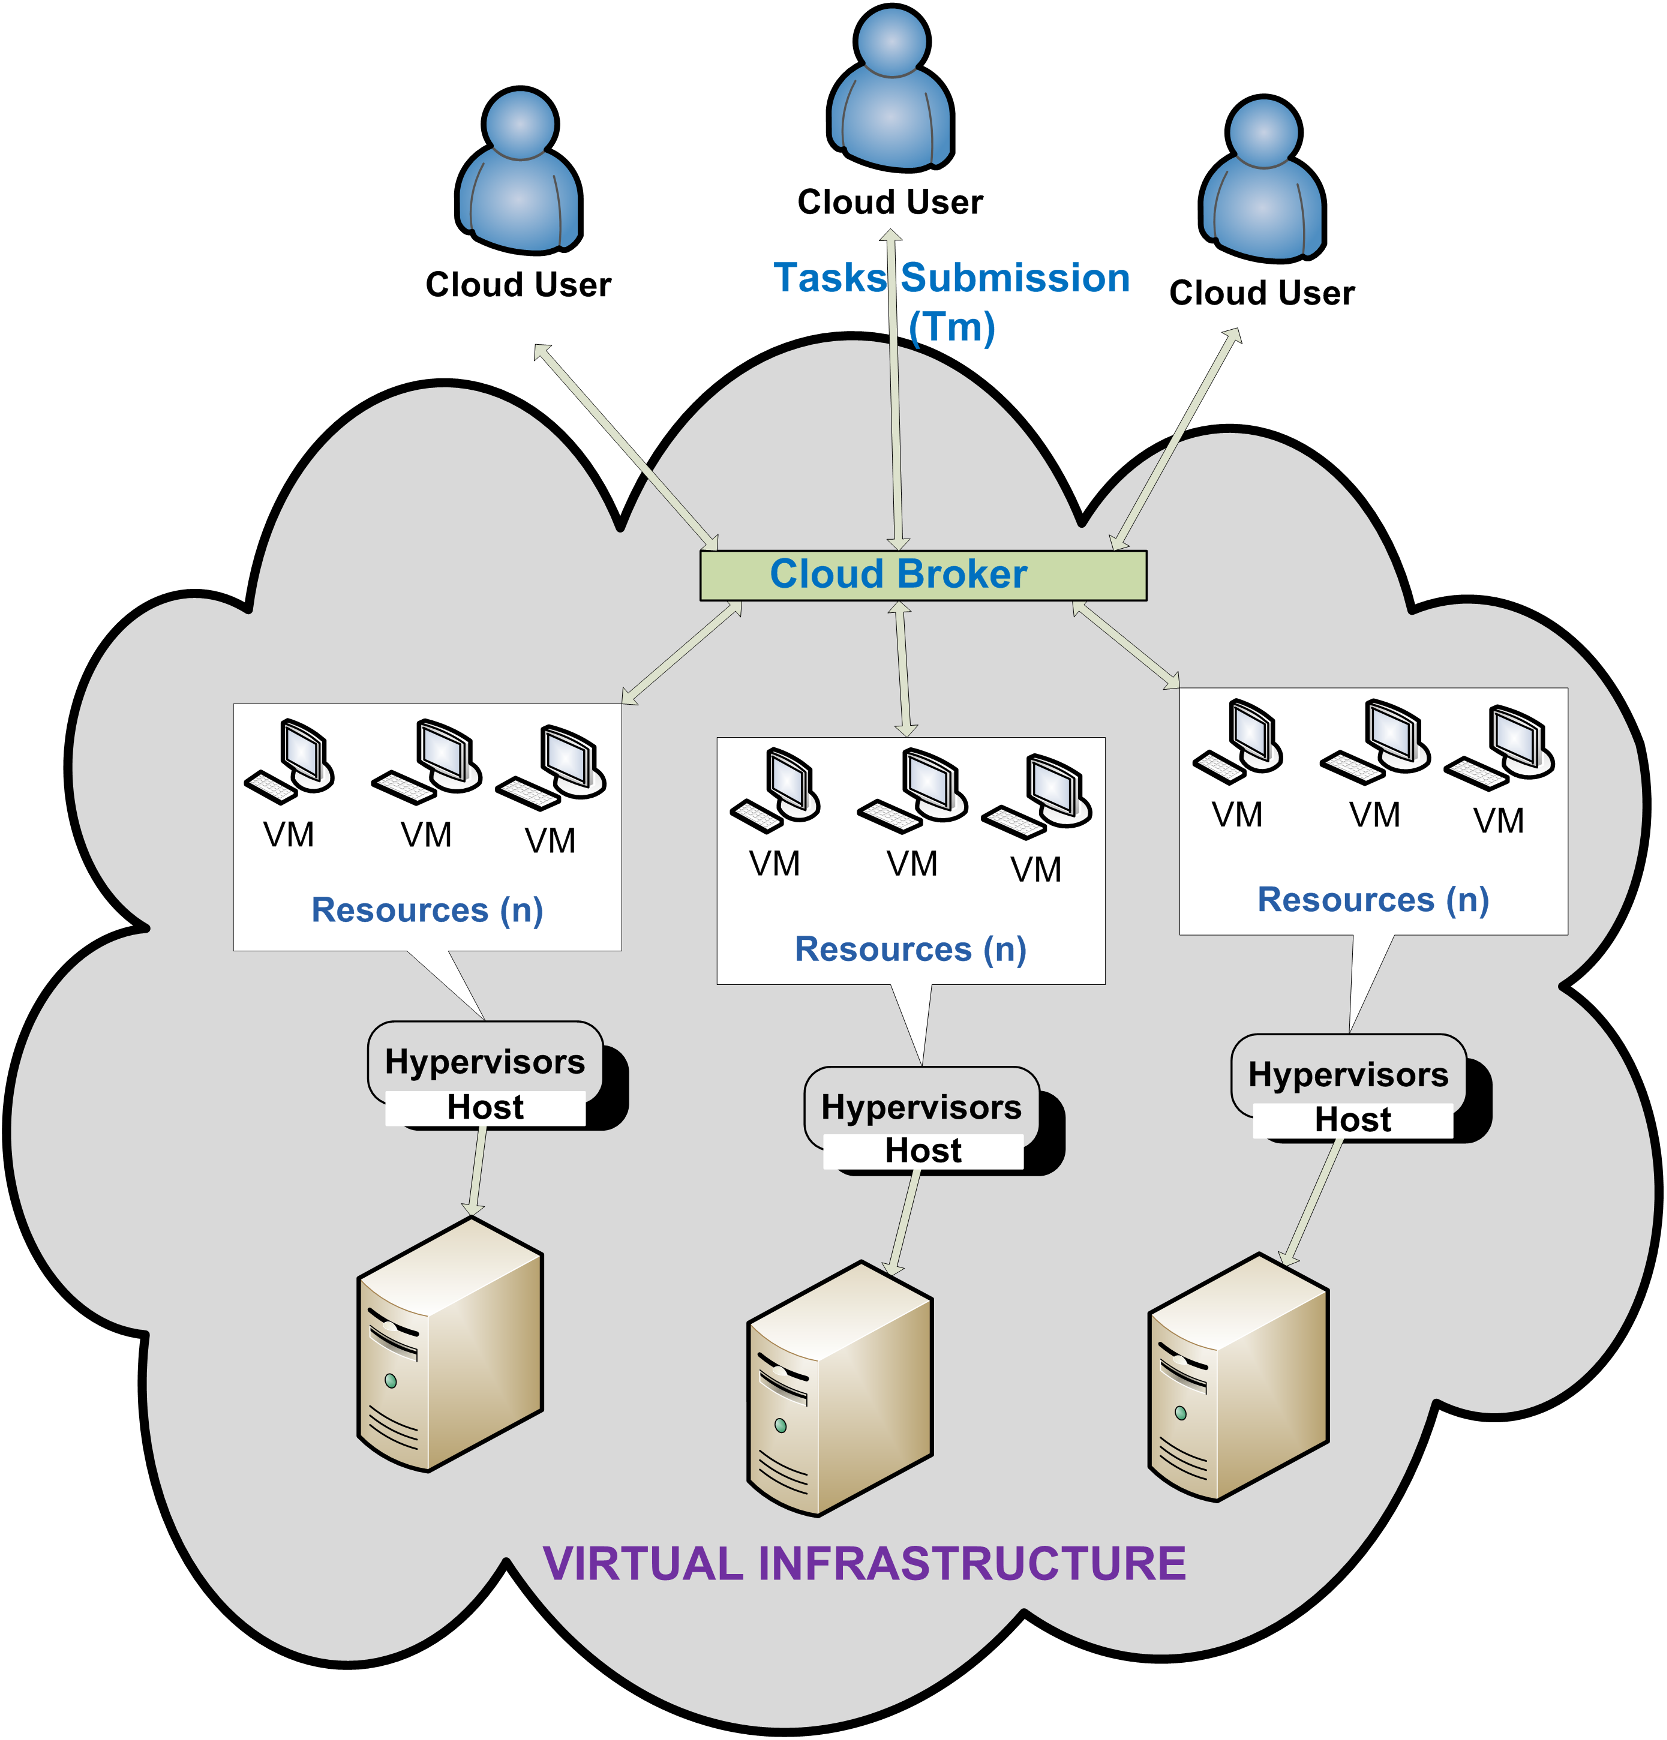
\includegraphics[scale=0.7]{images/cloud_computing_usecase.png}
	\caption{Lập lịch trong môi trường cloud computing}
	\label{fig:scheduling_in_cloud}
	\source{\cite{33}}
\end{figure}
Như trong hình~\ref{fig:scheduling_in_cloud}, các công việc tính toán sẽ được gửi từ người dùng bằng các ứng dụng web, api, ... tới trung tâm máy chủ, hay chính là cloud. \textbf{Cloud broker}, là trung gian giữa hệ thống tính toán của máy chủ với các ứng dụng bên ngoài, có nhiệm vụ tiếp nhận, quản lý và phân phối tới các tài nguyên trong cloud. Việc phân phối này sẽ sử dụng bộ lập lịch (scheduler) để tối ưu tài nguyên sử dụng và các thông số đánh giá chất lượng của dịch vụ (qualities of services). Sau đấy các công việc (từ giờ trở đi sẽ được viết theo tên tiếng anh, tasks) sẽ được chuyển tới máy tính ảo tương ứng với kết quả của việc lập lịch, và được thực thi trên đó. Các tài nguyên vật lý sẽ được quản lý bằng cách ảo hóa thành các tài nguyên ảo, nhằm mục đích dễ phân chia và mở rộng.
\begin{figure}[h!]
	\centering
	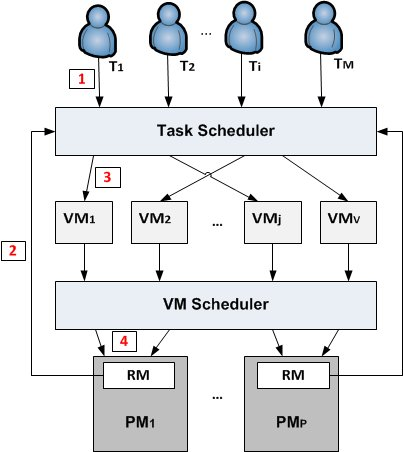
\includegraphics[scale=0.5]{images/scheduling_types.jpg}
	\caption{Các thành phần lập lịch}
	\label{fig:2}
	\source{\cite{34}}
\end{figure}
Như vậy, với công nghệ ảo hóa (virtualization computing), để thực thi task được gửi từ người dùng thì ta cần có 2 bô lập lịch sau (hình~\ref{fig:2}): 
\begin{itemize}
	\item \textbf{Task Scheduler}: là chương trình phân phối tasks đến các máy tính ảo.
	\item \textbf{VM Scheduler}: là chương trình quyết định xem các máy tính ảo được triển khai trên các máy chủ vật lý nào.
\end{itemize}
Đồ án này nghiên cứu về task scheduler, do đó từ giờ trở đi khi thuật ngữ "scheduler" được nhắc đến mà không ghi cụ thể thì ta hiểu rằng nó là "task scheduler".

\subsection*{Tiêu chí tối ưu}
Trước tiên, bài toán lập lịch trong môi trường cloud computing là một bài toán tối ưu.
Ta biết rằng mục đích của việc lập lịch là tối ưu việc sử dụng tài nguyên, tăng hiệu năng của hệ thống và xa hơn là tăng doanh thu cho doanh nghiệp. Có thể nói đó là những mục tiêu "vĩ mô", tạo nên nó là sự kết hợp của rất nhiều phần trong doanh nghiệp, và rất khó để đánh giá nếu chỉ tính dựa trên hiệu năng của bộ lập lịch. 
Do đó, ta cần đưa ra các tiêu chí, metrics mà dựa vào nó ta có thể đánh giá, so sánh giữa những thuật toán lập lịch với nhau. Dưới đây là một số hàm mục tiêu\cite{8}, thường được sử dụng trong nghiên cứu và phát triển: 
\begin{itemize}
	\item \textbf{makespan}: thời gian hoàn thành một khối lượng các công việc đã được xác định
	\item \textbf{cost}: chi phí để hoàn thành một khối lượng công việc 
	\item \textbf{throughput}: lượng công việc hoàn thành được trong một đơn vị thời gian 
	\item \textbf{load balancing}: sự cân bằng mật độ dữ liệu tại mọi thời điểm trong hệ thống cloud 
	\item \textbf{energy}: mức tiêu thụ năng lượng của hệ thống để hoàn thành một khối lượng công việc
	\item \textbf{execution time}: thời gian thực thi tasks
	\item \textbf{response time}: thời gian chờ đợi phản hồi từ người dùng
	\item \textbf{qualities of service}: được đưa ra trong thỏa thuận cấp độ dịch vụ (SLA – Service Level Agreement), có thể bao gồm các ràng buộc về deadline, makespan, cost, ...
\end{itemize}
\subsection*{Bài toán lập lịch}
Xét hệ thống có M máy tính ảo, cần thực thi N tasks.
\begin{itemize}
	\item $vms = \{vm_{1}, vm_{2}, ..., vm_{M}\}$ là tập M vector thông tin của máy ảo
	\item $tasks = \{task_{1}, task_{2}, ..., task_{N}\}$ là tập N vector thông tin của tasks
	\item $\mathcal{S} = \{task_{i} \rightarrow vm_{j}\}$ là cách ghép cặp N tasks tới M máy ảo
	\item $\mathcal{U} = \{\mathcal{S}\}$, là tập hợp tất cả các cách ghép cặp
	\item $\mathcal{F}(S)$ là hàm tối ưu (có thể là giá trị vô hướng hoặc là vector trong trường hợp xét nhiều hơn 2 mục tiêu) của một cách ghép cặp.
\end{itemize}
Không mất tính tổng quát, giả sử bài toán yêu cầu cực tiểu hóa hàm mục tiêu, vì nếu ngược lại thì có thể đổi dấu của nó. Ta cần tìm $\mathcal{S^{*}}$ sao cho: 
\begin{equation*}
	\mathcal{S^{*}} = argmin_{\mathcal{S} \in \mathcal{U}}\mathcal{F}(\mathcal{S})
\end{equation*}

\section{Lập lịch thời gian thực trong môi trường cloud computing}
\label{realtime}
Giống như bài toán lập lịch động được nhắc đến trong~\ref{dynamic_scheduling}, nhiều thông tin của task và môi trường có thể thay đổi trong thời gian thực. Hơn nữa, ở trong môi trường cloud computing, các công việc được gửi tới từ người dùng rất đa dạng, và có thêm mức ưu tiên cho từng công việc, khiến cho việc xác định chính xác một số thông tin của task như thời gian thực thi là không thể. Như ở trong bộ dữ liệu google trace v2\cite{18}, không thể xác định thời gian thực thi của tasks khi chúng đến hệ thống, và con số về tài nguyên được yêu cầu với tài nguyên thực tế sử dụng của các tasks là không đồng nhất\cite{17}.\\
Trong hệ thống thực tế, số lượng tasks đến theo thời gian là vô hạn. 
\begin{itemize}
	\item $vms = \{vm_{1}, vm_{2}, ..., vm_{M}\}$ là tập M vector thông tin của máy ảo
	\item $tasks = \{task_{1}, task_{2}, ..., task_{N}\}$ là tập vector thông tin của tasks với \\ $N \to \infty$
	\item $times = \{t_{1}, t_{2}, ..., t_{N}\}$ là tập thời gian đến hệ thống của các task với chỉ số tương ứng
	\item $constraints = \{r_{1}, r_{2}, ..., r_{N}\}$ là tập ràng buộc tương ứng với các tasks
\end{itemize}
Trong bài toán lập lịch này, trạng thái tài nguyên của hệ thống sẽ rất khó xác định. Có hai nguyên nhân chính sau: 
\begin{itemize}
	\item tài nguyên được yêu cầu bởi các task với tài nguyên thực tế chúng sử dụng là không đồng nhất
	\item sự thay đổi trạng thái của task trong quá trình chạy (khi task đang thực thi thì bị dừng lại để nhường tài nguyên cho task có ưu tiên cao hơn, hoặc kết thúc công việc)
\end{itemize}
Ngoài ra còn có sự thay đổi trong cấu hình của hệ thống. Bên cạnh sự không chắc chắn về trạng thái tài nguyên, các thông tin về thời gian chạy của task cũng không xác định. Điều này làm cho một số thuật toán phát triển trước đó như min-min hay max-min không áp dụng được. Load-balancing cũng trở lên tồi tệ do trạng thái tasks thay đổi quá nhanh làm mất cân bằng giữa các máy tính trong hệ thống. 

\section{Mục tiêu của đồ án nghiên cứu}
Như đã trình bày trong~\ref{realtime}, sự không chắc chắn về trạng thái tài nguyên cùng với việc thiếu thông tin về thời gian thực thi của các tasks khiến cho việc lập lịch không thể tối ưu một vài chỉ số như makespan, throughput, load-balancing. Đồ án này có mục tiêu cải thiện các vấn đề trên, cụ thể: 
\begin{enumerate}
	\item Xác định các nguyên nhân làm cho các thuật toán lập lịch cổ điển không tối ưu cho bài toán lập lịch thời gian thực trong môi trường điện toán đám mây 
	\item Đưa ra mô hình ước lượng trạng thái tài nguyên trong quá trình hoạt động của hệ thống và cơ chế lập lịch để sự thay đổi trạng thái các tasks không "phá vỡ" load-balancing của hệ thống
	\item Cài đặt và đánh giá mô hình đề xuất 
\end{enumerate}
Với mục tiêu thứ nhất, nhiều mô hình học máy đã được xem xét, trong đó mô hình đồ thị xác suất Bayesian là một lựa chọn phù hợp để biểu diễn các điều kiện độc lập và phụ thuộc giữa các thành phần trong hệ thống, dễ dàng học "tri thức" từ dữ liệu và đưa ra suy luận trong thời gian chấp nhận được. Tiếp theo, thuật toán \textbf{bestfit} kết hợp với các kết quả ước lượng trước đó sẽ đưa ra lời giải mà cải thiện load-balancing của hệ thống. 
\section{Cấu trúc đồ án}
Đồ án này được chia thành các phần chính như sau: 
\begin{itemize}
	\item Chương~\ref{Introduction} giới thiệu toản quan về bài toán nghiên cứu.
	\item Chương~\ref{related_works} tóm tắt ngắn gọn về các kiểu lập lịch và những thuật toán đã được nghiên cứu trước đây.
	\item Chương~\ref{Bayesian_network} giới thiệu về đồ thị xác suất Bayesian.
	\item Chương~\ref{Scheduling_model} mô tả mô hình lập lịch đề xuất.
	\item Chương~\ref{Experiments} là thực nghiệm và đánh giá. 
	\item Chương~\ref{Conclusion} Kết luận và định hướng nghiên cứu. 
\end{itemize}
Phạm vi đồ án bao gồm: 
\begin{itemize}
	\item Mô phỏng môi trường hoạt động Cloud bằng công cụ CloudSim~\cite{30}
	\item Thu thập và trích rút dữ liệu mô phỏng từ API của Google 
	\item Cài đặt thuật toán đề xuất và một vài thuật toán liên quan trong môi trường mô phỏng 
	\item So sánh hiệu quả lập lịch giữa thuật toán đề xuất và các thuật toán khác 
\end{itemize}

\newpage
\chapter{Các dạng lập lịch và nghiên cứu liên quan}
\label{related_works}
\section{Các phương pháp lập lịch}
Trong \cite{8}, tác giả đã phân chia các thuật toán lập lịch dưới dạng cây phân cấp như hình~\ref{fig:3}.
\begin{figure}[h!]
	\centering
	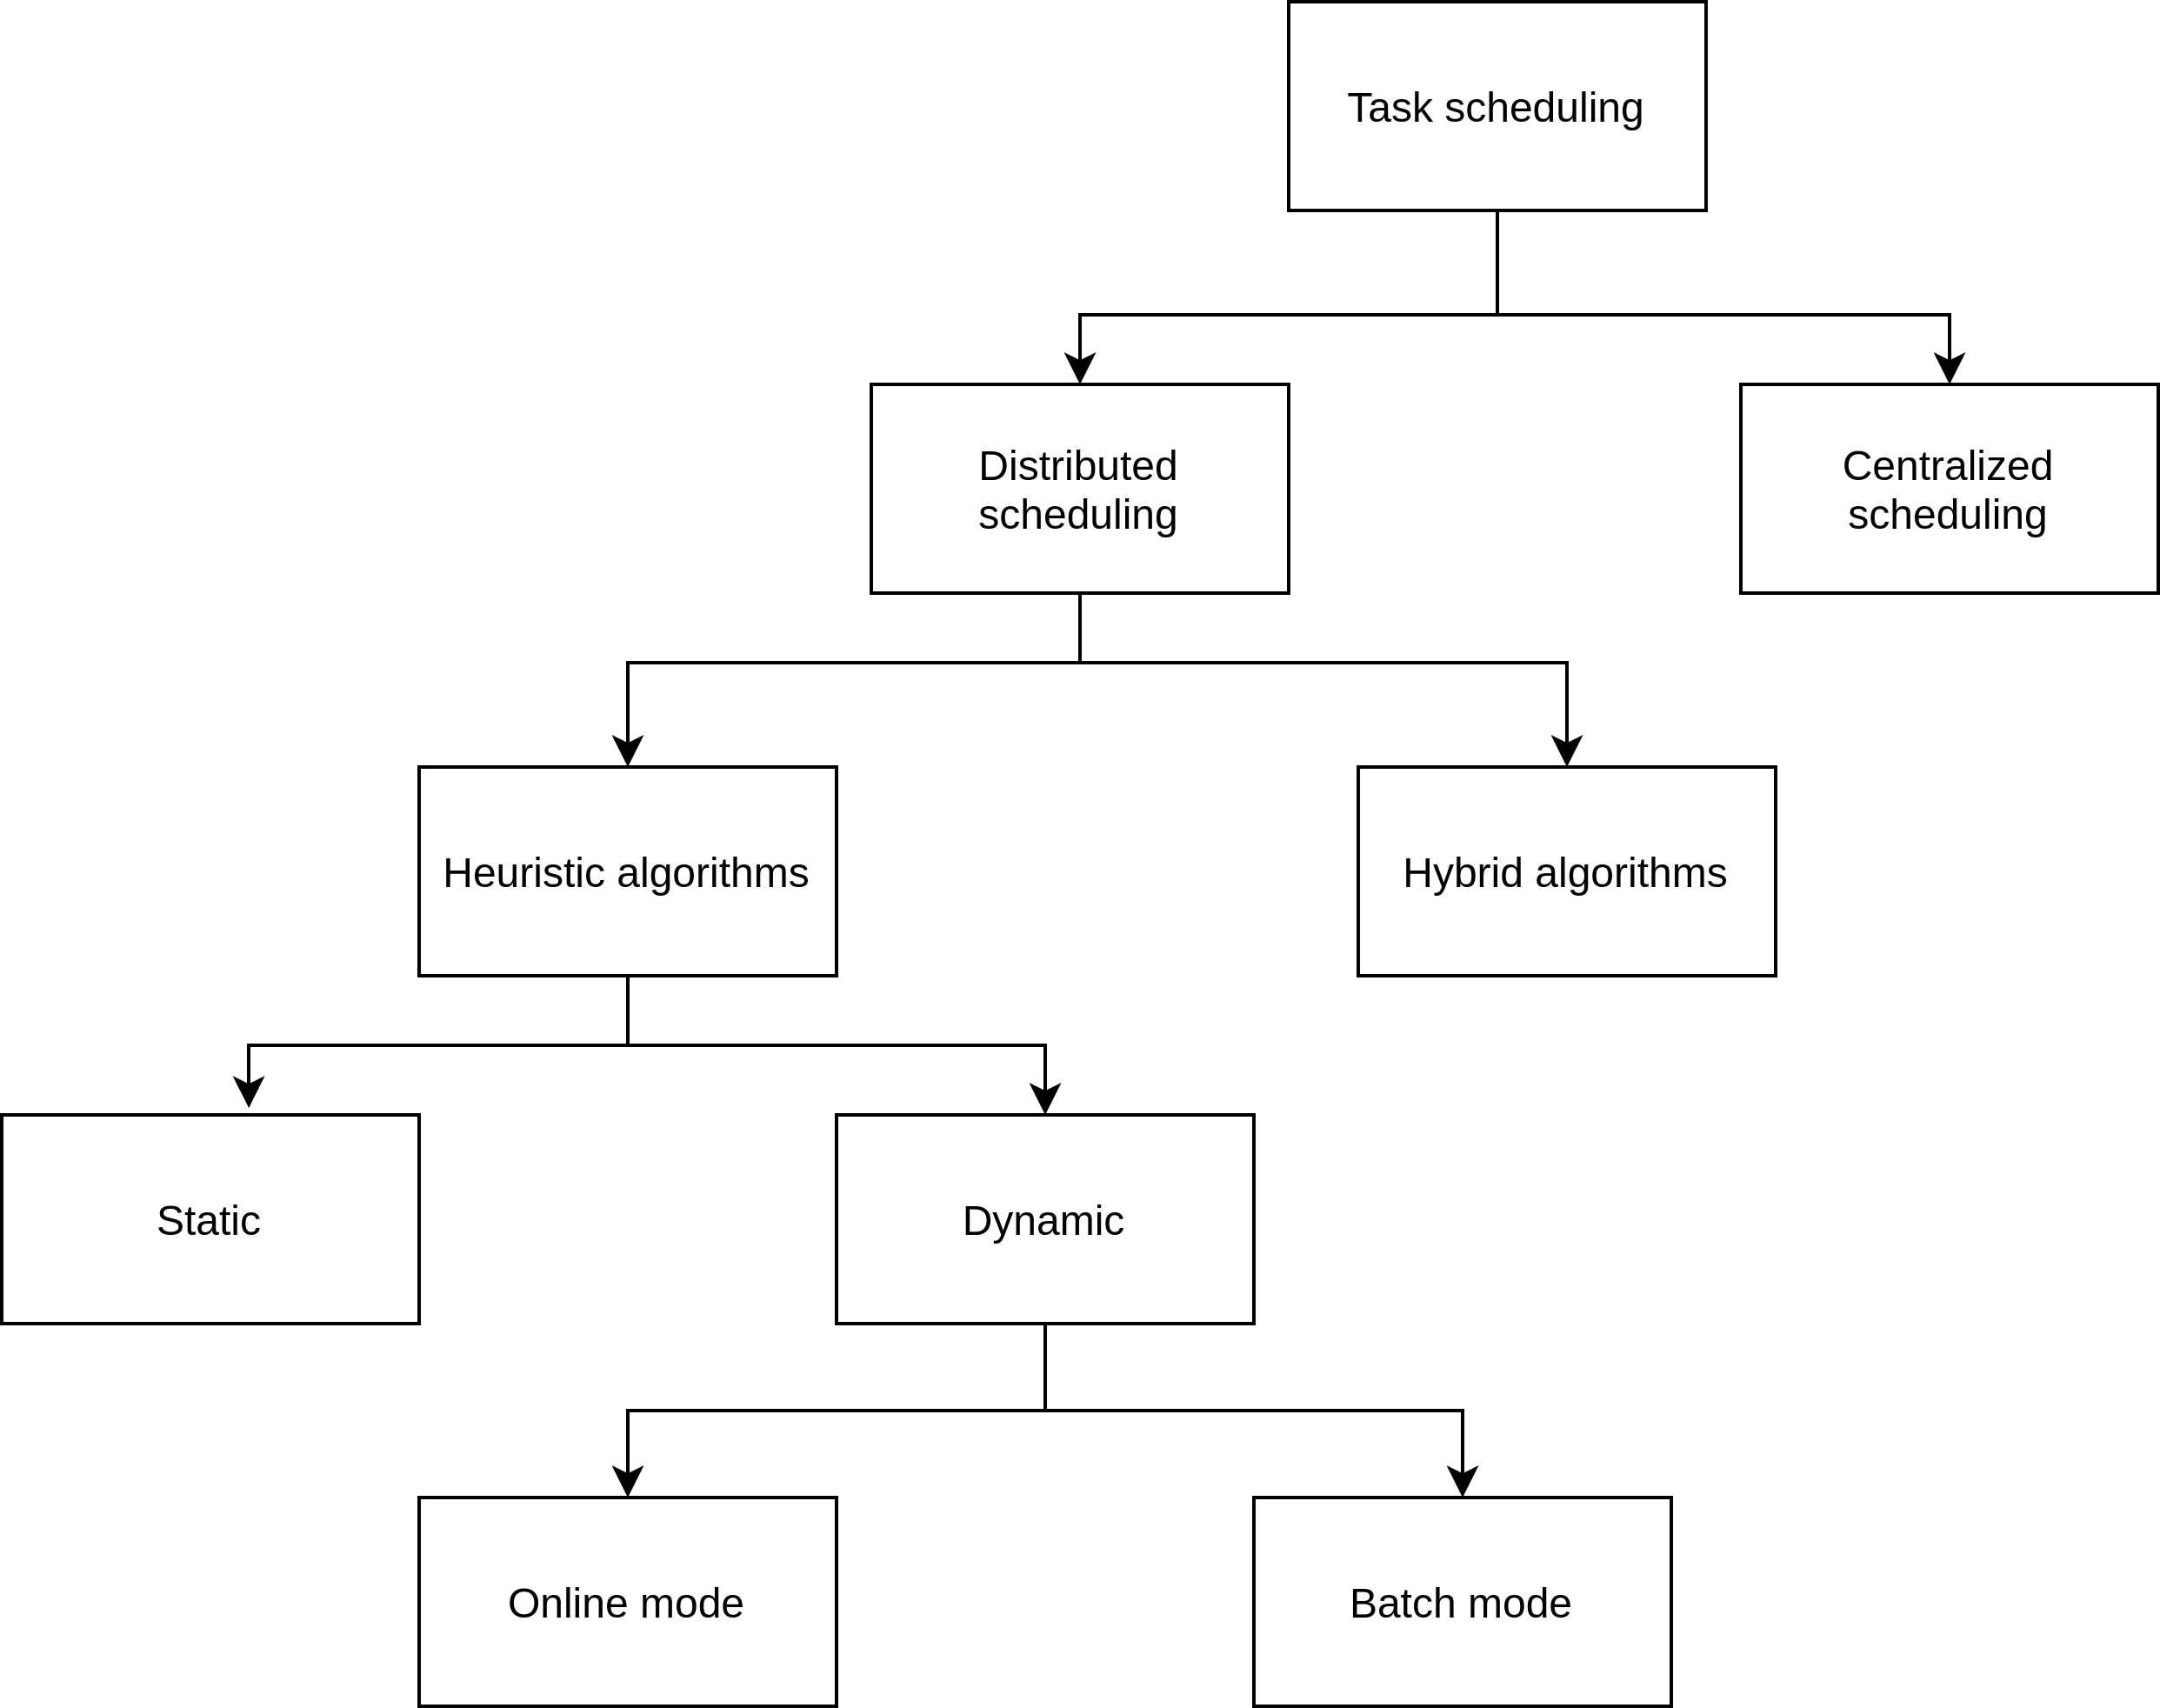
\includegraphics[scale=0.6]{images/scheduling_classification.png}
	\caption{Các phương pháp lập lịch}
	\label{fig:3}
\end{figure}
Đồ án này tập chung giải quyết bài toán \textbf{batch mode}, do đó ở các phần như \textbf{centralized scheduling}, thực tế sẽ được phân thành nhiều phần cụ thể hơn, nhưng do mục đích của ta không phải là nghiên cứu tổng quan giữa các kiểu bài toán lập lịch nên sẽ không làm rõ ở đây. 

\subsection{Centralized scheduling}
\textbf{Centralized scheduling}\cite{9} là kiểu bài toán lập lịch khi chỉ có một bộ lập lịch chung cho tất cả các task đến hệ thống. Bộ lập lịch này sẽ quản lý thông tin của toàn bộ cluster, thường các cluster này sẽ ở gần nhau theo vị trí địa lý. 

\subsection{Distributed scheduling}
\textbf{Distributed scheduling}\cite{9} là trong trường hợp sẽ có nhiều bộ lập lịch được đặt ở các vị trí chung gian giữa người dùng và các cluster của hệ thống. Các bộ lập lịch này sẽ trao đổi thông tin với toàn bộ cluster, định tuyến và phân chia tài nguyên cho các task. Ưu điểm của mô hình này so với \textbf{centralized scheduling} là dễ dàng mở rộng quy mô máy chủ, người dùng, nhưng có hạn chế là do bộ lập lịch cách xa các cluster nên sẽ có độ trễ trong khi trao đổi thông tin. 

\subsection{Hybrid algorithm}
\textbf{Hybrid scheduling algorithms} là nhóm các thuật toán mà kết hợp nhiều phương pháp khác nhau để tối ưu nhiều tiêu chí cùng một lúc. Ví dụ như trong \cite{12}, tác giả sử dụng "lexi-search" để đưa ra lời giải tối ưu 
\textbf{execution time}, \textbf{load balancing}.

\subsection{Heuristic algorithms}
Trong \cite{8}\cite{10}, \textbf{heuristic scheduling} là việc lập lịch dựa vào những giải thuật heuristic như 
PSO, Genetic, ... Trong môi trường phân tán, các thông tin về máy chủ và task có thể là không đồng nhất, do đó để tìm được lời giải tối ưu tuyệt đối cho bài toán là vô cùng khó, và đôi khi là không cần thiết. Các thuật toán heuristic sẽ tìm cho ta lời giải "chấp nhận được" trong thời gian cho phép.

\subsection{Static scheduling}
\textbf{Static scheduling}, hay là bài toán lập lịch tĩnh, các tasks sẽ đến hệ thống vào cùng một thời điểm, không bị ảnh hưởng bởi các yếu tố liên quan đến hệ thống tài nguyên. Các thông tin về cấu trúc của tasks, thông tin về môi trường, khối lượng công việc đều được xác định. Tất cả các tasks đều sẽ được phân phối tài nguyên trước khi thực thi. Với loại bài toán này, một số giải thuật "cổ điển" như "First Come First Serve", "Round Robin" đã được ứng dụng trong rất nhiều hệ thống. Ưu điểm của các giải thuật này là đơn giản, dễ triển khai, nhưng nhược điểm là không thể tối ưu các tiêu chí được để cập trước đó. Ngoài ra, min-min và max-min là hai thuật toán heuristic cơ bản được áp dụng phổ biến.
\begin{itemize}
	\item \textbf{Min-min}\cite{13} là cách lựa chọn task có execution time nhỏ nhất để gán vào máy tính tương ứng trước tiên. Những task dài sẽ được gán sau cùng, và nếu hệ thống không đủ tài nguyên thì chúng phải chờ đợi đến khi tài nguyên khả dụng. Ta đã biết rằng các tasks dài mới là thành phần quyết định đến chỉ số makespan, do đó thuật toán này chưa tối ưu về makespan, nhưng bù lại, chúng làm tăng throughput, tức là số lượng task hoàn thành trong một đơn vị thời gian. Vấn đề đói tài nguyên cũng sẽ khiến thuật toán này trở lên "tồi tệ", do có thể xảy ra trường hợp task "dài" sẽ luôn trong tình trạng không đủ tài nguyên do chúng luôn được lập lịch sau cùng. 
	\item \textbf{Max-min}\cite{14} có một chút ngược lại với min-min. Thuật toán này lựa chọn task có execution time lớn nhất được phân phối tài nguyên trước. Với cách lập lịch này thì các task "ngắn" sẽ được sắp xếp cuối cùng, và cũng có nguy cơ bị "đói tài nguyên", tức là sau nhiều lần lập lịch vẫn chưa được thực thi do thiếu tài nguyên. Do các task "dài" được sắp xếp trước nên makespan sẽ nhỏ hơn so với min-min, nhưng throughput cũng tương ứng giảm. 
\end{itemize}

\subsection{Dynamic scheduling}
\label{dynamic_scheduling}
Trong \textbf{dynamic scheduling} (lập lịch động), yếu tố \textbf{dynamic} được xem xét ở cả tasks và tài nguyên hệ thống. 
Tasks sẽ đến hệ thống theo thời gian, và có nhiều yếu tố ảnh hưởng đến nó trong quá trình chạy. Ví dụ như task có thể bị fail khi tài nguyên hệ thống không đủ và nhường cho task khác, hay thời gian chạy của task là không thể xác định trước. Hơn nữa, các máy tính có thể bị lỗi, dừng hoạt động trong quá trình chạy, dẫn đến sự thay đổi về tài nguyên khả dụng trong quá trình lập lịch. \\
Thông thường, các thuật toán lập lịch động được chia làm 2 hướng tiếp cận chính\cite{15} như sau: 
\begin{itemize}
	\item \textbf{Online mode}
	\item \textbf{Batch mode}
\end{itemize}
Với \textbf{online mode}, task được lập lịch ngay sau khi nó đến hệ thống, và quyết định lập lịch đó sẽ không bị thay đổi. Cách làm này phù hợp với các trường hợp có tỉ lệ task đến hệ thống thấp\cite{16}. Một số thuật toán lập lịch trong trường hợp này như sau: 
\begin{itemize}
	\item \textbf{Minimum completion time (MCT)} lựa chọn máy tính mà có thời gian hoàn thành công việc sớm nhất cho task
	\item \textbf{Minimum execution time (MET)} lựa chọn máy tính có thời gian thực thi task là nhỏ nhất
\end{itemize}
Với \textbf{batch mode}, sau khi đến hệ thống,  các task sẽ đến một hàng đợi, sau một khoảng thời gian (interval time) thì hệ thống sẽ lập lịch cho các task trong tập đó. Để lựa chọn thời gian đợi cho hàng đợi, có 2 phương án sau: 
\begin{itemize}
	\item \textbf{Regular time interval}: thực hiện lập lịch sau một khoảng thời gian cố định (vd: 100s).
	\item \textbf{Fixed count}: thực hiện lập lịch khi thỏa mãn 1 trong 2 điều kiện sau: 
	\begin{itemize}
		 \item Một task mới đến khiến cho lượng task trong tập đang đợi lớn hơn hằng số đặt trước
		 \item Thời gian chờ đã lớn hơn hoặc bằng hằng số định trước
	\end{itemize}
\end{itemize}

\section{Các nghiên cứu liên quan}
% 5-7 pages 
% Tìm hiểu thuật toán lập lịch của google, microsoft, amazone, facebook
Đã có nhiều framework được phát triển để giải quyết bài toán lập lịch thời gian thực trong môi trường phân tán.\\
Với ngữ cảnh các tasks đến hệ thống với n máy ảo theo phân phối Poisson, trong \cite{21}, bộ lập lịch chọn ngẫu nhiên d máy ảo và gán task tới máy ảo có số lượng task đang đợi là ít nhất, \textit{Michael Mitzenmacher} đưa ra kết luận rằng makespan của d = 2 sẽ được cải thiện theo hàm mũ so sánh với d = 1, bên cạnh đó thì d = 3 chỉ tốt hơn theo hàm hằng số so với d = 2. Điểm yếu của thuật toán này là trong trường hợp các tasks được tính toán song song, tức là được thực thi trong nhiều máy tính khác nhau thì việc lựa chọn như trên sẽ làm tăng thời gian hoàn thành công việc. \\
Trong \cite{20}, tác giả đề xuất Sparrow - một mô hình lập lịch hướng tới các hệ thống phân tích dữ liệu lớn, cải tiến nhược điểm trong trường hợp của các tasks cần được song song hóa của phương pháp trước phía trên. Mục tiêu của Sparrow là giảm độ trễ trong quá trình lập lịch cho hệ thống phân tán tính toán song song. Sparrow sử dụng phương pháp được đề xuất trong\cite{22} để lập lịch đảm bảo điều kiện song song hóa giữa các tasks. Sparrow đã được phát triển như một plugin của Apache Spark và tỏ ra hiệu quả so với thuật toán lập lịch nguyên bản của Spark khi số lượng tasks tại một thời điểm lớn nhưng thời gian thực thi ngắn. \\
Một cách lập lịch phổ biến khác và được áp dụng trong Borg\cite{17}\cite{19} - một hệ thống quản lý trung tâm máy chủ của Google, đã bỏ qua phần ước lượng thời gian thực thi trong quá trình lập lịch. Các task đến hệ thống có 3 mức độ ưu tiên là \textbf{free}, \textbf{production}, \textbf{monitor}, lần lược theo mức độ tăng dần. Một máy tính sẽ dừng lại công việc ở mức ưu tiên thấp để dành tài nguyên cho cái có mức ưu tiên cao hơn trong trường hợp không đủ tài nguyên. Cụ thể, việc lập lịch được chia làm 2 giai đoạn: 
\begin{itemize}
	\item \textbf{feasible checking}: tìm các máy tính thỏa mãn ràng buộc của task (thường ràng buộc về thư viện) và đủ tài nguyên (tính cả phần tài nguyên được sử dụng cho free tasks)
	\item \textbf{scoring}: tính "điểm" cho các máy tính, dựa trên một số tiêu chuẩn như số lượng tasks bị dừng lại do thiếu tài nguyên, mức độ cân bằng tải giữa các máy tính để lựa chọn máy tính tốt nhất cho task
\end{itemize}
Quá trình scoring sử dụng một vài biến thể của thuật toán E-PVM\cite{23}, mục tiêu là đưa ra một giá trị chi phí mà tối ưu nó sẽ giúp ta đạt được load-balancing của hệ thống. Tuy vậy, việc đảm bảo load-balancing dẫn đến vấn đề phân mảnh bộ nhớ, khiến cho đôi khi tài nguyên dư thừa nhưng không sử dụng được. Ngoài ra, feasible checking và scoring cho từng task rất tốn kém, nên Borg đã sử dụng score caching, tức là lưu lại điểm cho đến khi các các thông tin về task đó hay máy tính tương ứng với nó bị thay đổi. Các tasks cũng được chia thành các nhóm dựa trên ràng buộc của chúng, tức là với 2 task nằm trong cùng một nhóm thì điều kiện để có thể thực thi là như nhau. Như vậy, thay vì tìm tập feasible machines cho từng task, ta sẽ tìm cho nhóm các tasks. Sau khi lập lịch, nếu có trường hợp bị đói tài nguyên thì các task với mức ưu tiên thấp sẽ bị dừng lại, hoặc bị hủy để nhường cho các task ưu tiên cao hơn. Các task bị hoãn đó sẽ quay lại hàng đợi cho lần lập lịch tiếp theo. Cơ chế dừng các task đang chạy để nhường cho các task mức ưu tiên cao hơn giúp cho người dùng dịch vụ trả phí sẽ có trải nghiệm tốt hơn với các dịch vụ khác của Google, nhưng điều này cũng gây ra sự lãng phí tài nguyên khi phải thực hiện cùng một công việc nhiều lần. Một kết quả được đưa ra trong \cite{24} cho thấy rằng việc chạy lại các công việc bị hoãn chiếm tới 60\% tài nguyên CPU của hệ thống.  \\
Trong \cite{25}, trong trường hợp số lượng máy tính ảo có thể thay đổi, tác giả đề xuất mô hình lập lịch 2 giai đoạn để lựa chọn cấu hình máy ảo trong hệ thống và phân phối công việc. Cụ thể, trong giai đoạn 1, tasks đến hệ thống sẽ được gán nhãn với các kiểu máy tính dựa theo tiêu chí các yêu cầu của tasks được đáp ứng trong kiểu máy tính đó. Sau đó với mỗi kiểu máy tính, ta sẽ tạo ra một số lượng máy ảo để thực thi các tasks được gán nhãn tương ứng. Giai đoạn 2 chính là phân phối các tasks vào máy tính ảo trùng nhãn với nó. Với mô hình lập lịch này, ta có thể tận dùng tài nguyên hệ thống tối ưu hơn dựa vào việc tự lựa chọn cấu hình cụm máy tính ảo, phân chia phù hợp các kiểu của tasks. Tuy nhiên, tác giải chỉ sử dụng tỉ lệ giữa các kiểu máy tính để đưa ra quyết định số lượng máy tính ảo được tạo ra với các kiểu tương ứng đó. Điều này sẽ khiến cho sự phân phối số lượng máy ảo vào các nhóm trở nên không hợp lý khi số lượng nhóm tăng lên và thông tin của task phức tạp hơn. \\
Trong \cite{26}, nhóm nghiên cứu đề xuất phương pháp mô phỏng Monte Carlo để phân chia số lượng máy tính ảo vào các nhóm kiểu máy tính để cải thiện giai đoạn 1 của thuật toán phía trước, nhưng với giải pháp này thì thời gian là một vấn đề do độ chính xác tỉ lệ thuận với số lần ta mô phỏng. Để không phải lặp lại việc mô phỏng nhiều lần, tác giả đề xuất một độ đo tương đồng giữa hai lần lập lịch, nếu trạng thái hiện tại có độ đo không quá sai khác với trạng thái trước đó thì nó sẽ dùng kết quả của lần lập lịch trước. \\
\subsection*{Nhận xét}
Các mô hình lập lịch trên, tùy từng mô hình mà chúng có mục tiêu tối ưu riêng, nhưng đều hướng tới tăng chất lượng của dịch vụ và hiểu quả việc sử dụng tài nguyên. Tuy vậy, một số vấn đề sau đây vẫn chưa được xem xét cẩn thận khi thực hiện lập lịch trong môi trường cloud: 
\begin{itemize}
	\item Sai số của hệ thống do sự trễ trong việc truyền thông tin.
	\item Sự tối ưu của các thuật toán nghiên cứu trước đó là tối ưu tại thời điểm lập lịch, không phải là tối ưu trong suốt quá trình chạy. Hệ thống Cloud gồm rất nhiều thành phần phức tạp liên tục thay đổi, điều này sẽ phá vỡ trạng thái tối ưu chấp nhận được - kết quả của việc lập lịch. 
	\item Một số tiêu chí tối ưu có tính chất "tương quan dương" với nhau, tức là nếu chỉ số này tốt hơn thì cái khác cũng tương tự. Ngược lại, một vài tiêu chí tối ưu là "sự đánh đổi", là tối ưu chỉ số này thì cần chấp nhận hạ chất lượng của tiêu chí còn lại. Tuy nhiên, "sự tương quan" và "sự đánh đổi" chưa được đo lường một cách cụ thể. 
\end{itemize}
Hướng tới giải pháp cho hai vấn đề đầu tiên, đồ án này đề xuất mô hình đồ thị xác suất mạng Bayesian để ước lượng kỳ vọng cho tài nguyên khả dụng của hệ thống cloud, từ đó đưa ra quyết định lập lịch. 


\newpage
\chapter{Mô hình đồ thị xác suất Bayesian}
\label{Bayesian_network}
% 3-4 pages
\section{Mô hình đồ thị xác suất}
%%
Mô hình đồ thị xác suất\cite{27}\cite{28} là một dạng mô hình xác suất biểu diễn các điều kiện độc lập giữa các biến ngẫu nhiên dưới dạng đồ thị, là mô hình toán học chứa các giả thuyết xác suất liên quan đến quá trình sinh ra dữ liệu.  Về mặt tổng quan, mô hình đồ thị xác suất giúp "phân rã" một phân phối xác suất nhiều chiều phức tạp thành một tập hợp của các phân phối đơn giản hơn với các điều kiện độc lập. Với ý tưởng tương tự như "chia để trị", các phân phối thành phần được tính toán đơn giản hơn và nhờ vậy ta có thể giảm thiểu độ phức tạp của bài toán.\\
\begin{figure}[h!]
    \centering
    \subfloat[\centering Đồ thị Bayesian]{{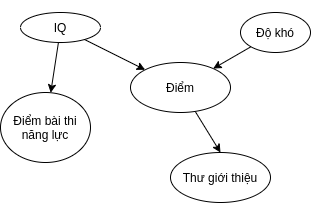
\includegraphics[width=5cm]{images/bayesian_network.png} }}%
    \qquad
    \subfloat[\centering Đồ thị Markov]{{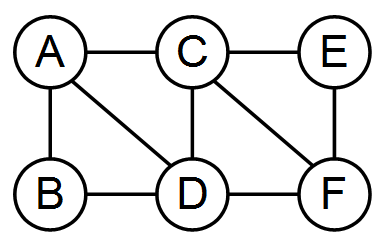
\includegraphics[width=5cm]{images/markov_network.png} }}%
    \caption{Mô hình đồ thị xác suất}%
    \label{fig:example}%
\end{figure}
Có hai cách biểu diễn thường dùng nhất với một phân phối, là biểu diễn thành đồ thị có hướng hoặc đồ thị vô hướng. Hai loại đồ thị này còn có tên lần lượt là \textbf{đồ thị Bayesian} và \textbf{đồ thị Markov}. Việc lựa chọn mô hình đồ thị nào phụ thuộc vào tình huống ta áp dụng. Cụ thể, các điều kiện độc lập giữa các biến ngẫu nhiên sẽ quyết định xem mô hình nào phù hợp với bài toán. Đôi khi cả hai loại đồ thị đều có thể đáp ứng, nhưng phần lớn trường hợp sẽ có một mô hình vượt trội hơn cái còn lại. \\
Ứng dụng của một mô hình đồ thị xác suất là trả lời các câu hỏi mang tính chất suy diễn khả năng xảy ra của các sự kiện dựa vào một số thông tin được cung cấp. Để làm được điều này, ta cần xây dựng một mô hình phù hợp với bối cảnh của bài toán, rồi đưa ra cơ chế tính xác suất dựa trên nhưng mô hình đó. Để có thể trả lời chính xác, mô hình của chúng ta cần có "tri thức" - thứ mà được xây dựng từ các các chuyên gia, hoặc là được rút ra từ dữ liệu. Việc trích xuất tri thức từ dữ liệu không còn mới lạ với cộng đồng khoa học hiện nay, và nó cũng trở thành một điểm mạnh của các mô hình đồ thị suy diễn. \\
Tóm lại, với một mô hình đồ thị xác suất, có ba vấn đề chính ta cần quan tâm: 
\begin{itemize}
	\item \textit{Representation}: cách biểu diễn các điều kiện độc lập dưới dạng đồ thị của các biến ngẫu nhiên (hình dạng của đồ thị)
	\item \textit{Inference}: cách tính xác suất của một sự kiện dựa trên đồ thị biểu diễn
	\item \textit{Learning}: cách trích xuất tri thức từ dữ liệu để xây dựng đồ thị
\end{itemize}
\section{Đồ thị Bayesian}
Trước khi tìm hiểu về mạng Bayesian, ta đề cập lại một số khái niệm của lý thuyết xác suất. \\
Kí hiệu $A \perp B$ | $C$ tức là A độc lập với B khi biết C, ở đây A, B, C đều là các biến ngẫu nhiên. \\
Ta có 
\[
	A \perp B \mid C \rightarrow P(A,B \mid C) = P(A \mid C)P(B \mid C)
\]
Phương pháp phân tích chuỗi xác suất Bayesian: 
\[
	P(A_{1}, A_{2}, ..., A_{n}) = P(A_{1})P(A_{2} \mid A_{1}) ... P(A_{n} \mid A_{1} ... A_{n-1})
\]
Với cách này, $P(A_{1}, A_{2}, ..., A_{n})$ được phân tích thành chuỗi các xác suất thành phần, trong đó có $P(A_{n} \mid A_{1} ... A_{n-1})$. Ta thấy rằng độ phức tạp khi tính $P(A_{n} \mid A_{1} ... A_{n-1})$ không hề thua kém $P(A_{1}, A_{2}, ..., A_{n})$, và sẽ tốn kém hơn nếu tính cả các nhân tử khác. Nhưng trong trường hợp giữa các biến tồn tại các điều kiện độc lập, mạng Bayesian có thể giúp làm đơn giản rất nhiều trong việc biểu diễn các phân phối trên.\\
Hãy xem xét một trường hợp cụ thể như sau. Một hệ thống thực hiện công việc được gửi tới từ người dùng. 
Việc thực thi các công việc đó làm trạng thái của hệ thống thay đổi. Tại thời điểm $t_{i}$, ta quan sát được trạng thái hệ thống là $S_{i}$, và dùng thông tin đó để lập lịch cho N công việc đang đợi ở hàng chờ. Thời gian lập lịch cho N công việc đó là D. Sau khi lập lịch xong, tại thời điểm $t_{i + 1} = t_{i} + D$, ta muốn biết trạng thái của hệ thống $S_{i+1}$ có thay đổi hay không. Trong bài toán này, tồn tại một số điều kiện xác suất sau: 
\begin{itemize}
	\item Trạng thái $S_{i+1}$ chỉ phụ thuộc vào trạng thái $S_{i}$ trước đó và khoảng thời gian giữa 2 lần quan sát 
	\item Thời gian lập lịch D chỉ phụ thuộc vào số lượng công việc cần lập lịch 
\end{itemize}
 
\subsection{Representation}
Ta sẽ biểu diễn bài toán trên dưới dạng một đồ thị Bayesian.
Đồ thị Bayesian là đồ thị có hướng không chu trình có các tính chất sau: 
\begin{itemize}
	\item Mỗi đỉnh biểu diễn cho một biến ngẫu nhiên
	\item Cạnh biểu diễn cho sự phụ thuộc giữa các biến ngẫu nhiên 
\end{itemize}
\begin{figure}[h!]
	\centering
	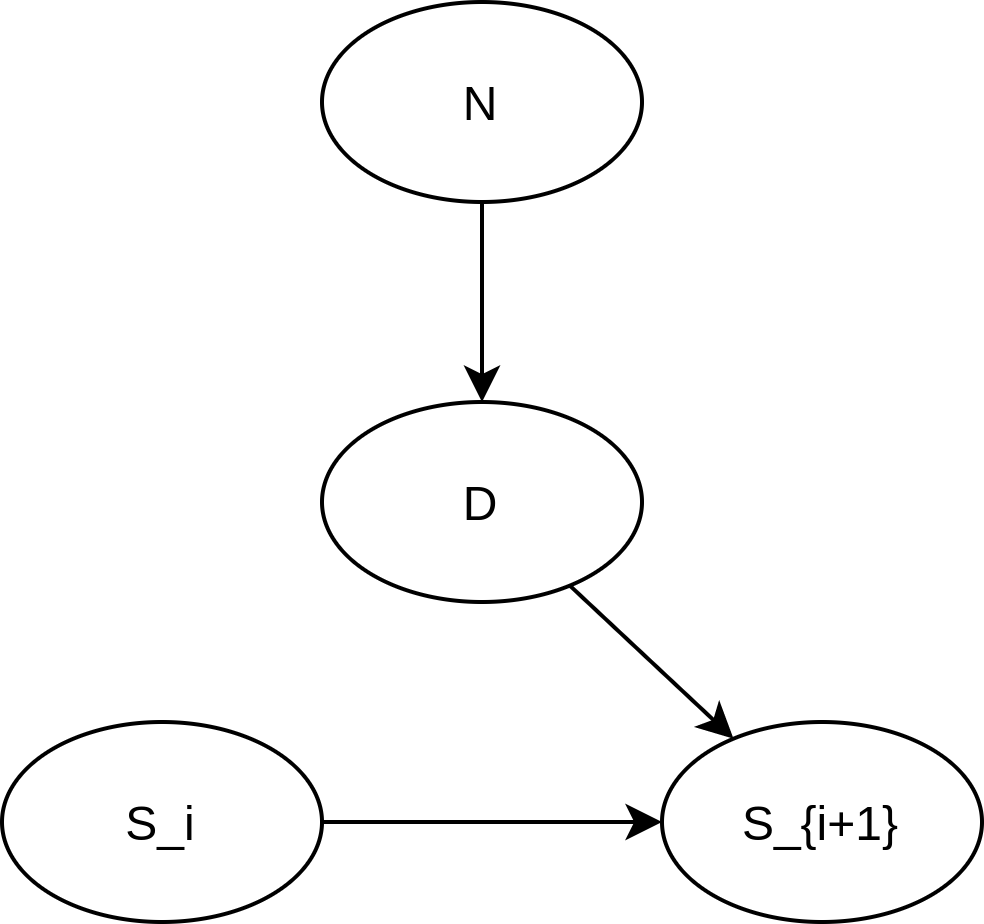
\includegraphics[scale=1.0]{images/bayesian_network_1.png}
	\caption{Mô hình đồ thị Bayesian}
	\label{fig:bayesian}
\end{figure}
Đồ thị Bayesian như trong hình~\ref{fig:bayesian} giúp ta biểu diễn một số điều kiện độc lập sau: 
\begin{itemize}
	\item $S_{i+1} \perp N \mid D$
	\item $S_{i} \perp \{D, N\}$
\end{itemize}
Từ đó, công thức chuỗi Bayesian cho các biến này được viết gọn như sau: 
\begin{align*}
	P(N, D, S_{i}, S_{i+1}) &= P(N) \times P(D \mid N) \times P(S_{i} \mid D, N) \times P(S_{i+1} \mid S_{i}, D, N) \\
							&= P(N) \times P(D \mid N) \times P(S_{i}) \times P(S_{i+1} \mid S_{i}, D)
\end{align*}
Ta có thể thấy, các phân phối thành phần trở lên đơn giản hơn rất nhiều so với phân phối chung ban đầu, nhờ vậy mà việc tính toán xác suất cũng trở lên dễ dàng hơn. 

\subsection{Inference}
\textbf{Inference} là quá trình trả lời các truy vấn liên quan đến xác suất xuất hiện của các sự kiện trong mạng Bayesian. Ví dụ, tập trạng thái của hệ thống là $S = \{s_{1}, s_{2}, s_{3}\}$, ta quan sát được có N = $n_{0}$ công việc sẽ được lập lịch, trạng thái hiện tại $S_{i} = s_{1}$, xác suất mà hệ thống không đổi trạng thái sau thời gian lập lịch là bao nhiêu? \\
Với truy vấn trên, ta cần tính: 
\begin{equation*}
	P(S_{i+1} = s_{1} \mid S_{i} = s_{1}, N = n_{0})
\end{equation*}
Gọi $\mathcal{D}$ là không gian sự kiện của biến D. Ta có thể phân tích như sau: 
\begin{align*}
	P(&S_{i+1} = s_{1} \mid S_{i} = s_{1}, N = n_{0}) = \sum_{d \in \mathcal{D}}P(S_{i+1} = s_{1}, D = d \mid S_{i} = s_{1}, N = n_{0}) \\
			&= \sum_{d \in \mathcal{D}}P(D = d \mid S_{i} = s_{1}, N = n_{0}) \times P(S_{i + 1} = s_{1} \mid D = d, S_{i} = s_{1}, N = n_{0}) \\
			&= \sum_{d \in \mathcal{D}}P(D = d \mid N = n_{0}) \times P(S_{i+1} = s_{1} \mid D = d, S_{i} = s_{1})		
\end{align*}
Dựa vào đồ thị, ta có thể tính được $P(D \mid N), P(S_{i+1} \mid S_{i}, D)$ và từ đó trả lời truy vấn bên trên. \\
Ngoài ra, còn có thể tìm xem $S_{i + 1}$ có khả năng nhận giá trị nào nhất, dựa vào truy vấn MAP (Maximum a Posteriori). 
\begin{equation*}
	MAP(S_{i+1} \mid S_{i} = s_{1}, N = n_{0}) = arg\underset{s}maxP(S_{i + 1} = s \mid S_{i} = s_{1}, N = n_{0})
\end{equation*}
Truy vấn trên đồ thị xác suất còn có một ưu điểm là ta có thể dựa vào cấu trúc dữ liệu đồ thị để giảm độ phức tạp trong quá trình tính toán truy vấn, điển hình như thuật toán Belief Propagation\cite{29}.\\

\subsection{Learning}
Trong nhiều trường hợp, con người không thể cung cấp được "kiến thức" cho đồ thị do khối lượng quá lớn và cần đòi hỏi sự hiểu biết về nhiều lĩnh vực, chuyên ngành. Ngoài ra, các phân phối của các biến có thể thay đổi theo thời gian. Khi đó, một giải pháp hiệu quả là chúng ta cho mô hình đồ thị học, trích rút tri thức từ bộ dữ liệu được sinh ra. \\
Trong bài toán ví dụ, khi ta muốn tính xác suất $P(N, D, S_{i}, S_{i+1})$, ta cần biết được giá trị của các thành phần $P(N)$, $P(D \mid N)$, $P(S_{i})$, $P(S_{i+1} \mid S_{i}, D)$, có thể hiểu là các tham số của mạng. Các giá trị này sẽ được cung cấp bởi những chuyên gia, hoặc sẽ được học từ dữ liệu.\\
Bài toán học trong đồ thị xác suất bản chất giống như một bài toán tối ưu. Xét $\Omega = \{x_{1}, x_{2}, ..., x_{m}\}$ là tập dữ liệu, $\theta$ là vector tham số của mạng, $\Theta$ là tập giá trị của $\theta$. Ta cần phải tìm giá trị $\theta^{*}$ sao cho likelihood của bộ dữ liệu đạt cực đại, tức là: 
\begin{equation*}
	\theta^{*} = arg\underset{\theta \in \Theta}maxP(\Omega \mid \theta)
\end{equation*}
Các phương pháp học trong mạng Bayesian đã được trình bày chi tiết trong \textit{Probabilistic Graphical Model: Princibles and Techniques}\cite{28}, nếu có thời gian xin hãy xem đến cuốn sách này. 

\newpage
\chapter{Mô hình lập lịch thời gian thực sử dụng mạng Bayesian ước lượng tài nguyên}
\label{Scheduling_model}
% 10-12 pages

\section{Bài toán thực tế}
Như đã trình bày trong ~\ref{realtime}, người dùng gửi các tasks đến cloud liên tục theo thời gian. Trong thực tế, người dùng sẽ gửi đến hệ thống các công việc dưới dạng các job, là tập các tasks có thể chạy độc lập với nhau. Do các tasks có thể chạy độc lập, nên ta coi như người dùng gửi các tasks đến hệ thống cùng một thời điểm, và chúng có quan hệ là có chung jobID (mã công việc người dùng gửi đến). Các tasks này sẽ được chia thành 2 loại\cite{17}: 
\begin{itemize}
	\item \textit{long-run}: các công việc mà không có thời điểm kết thúc, luôn chạy để xử lý những nhu cầu ngắn hạn của người dùng. Ví dụ: Gmail, Docs, web search, ...
	\item \textit{batch-job}: các công việc có thời gian chạy cụ thể, thường từ vài giây đến vài ngày, dao động tùy thuộc vào hiệu năng của hệ thống. Ví dụ: người dùng gửi đến công việc huấn luyện một mô hình học máy, hoặc chạy một script phân tích dữ liệu, ... 
\end{itemize}
Với kiểu lập lịch batch mode, các tasks phải đợi ở hàng chờ, rồi hệ thống lập lịch chạy cho tasks, và sau đó thì được đưa đến các máy tính ảo tương ứng vào thực thi công việc. Hình ~\ref{fig:flow} mô tả quá trình chuyển trạng thái của task trong thực tế.  
\begin{figure}[h!]
    \centering
    \subfloat[\centering Luồng hoạt động của hệ thống]{{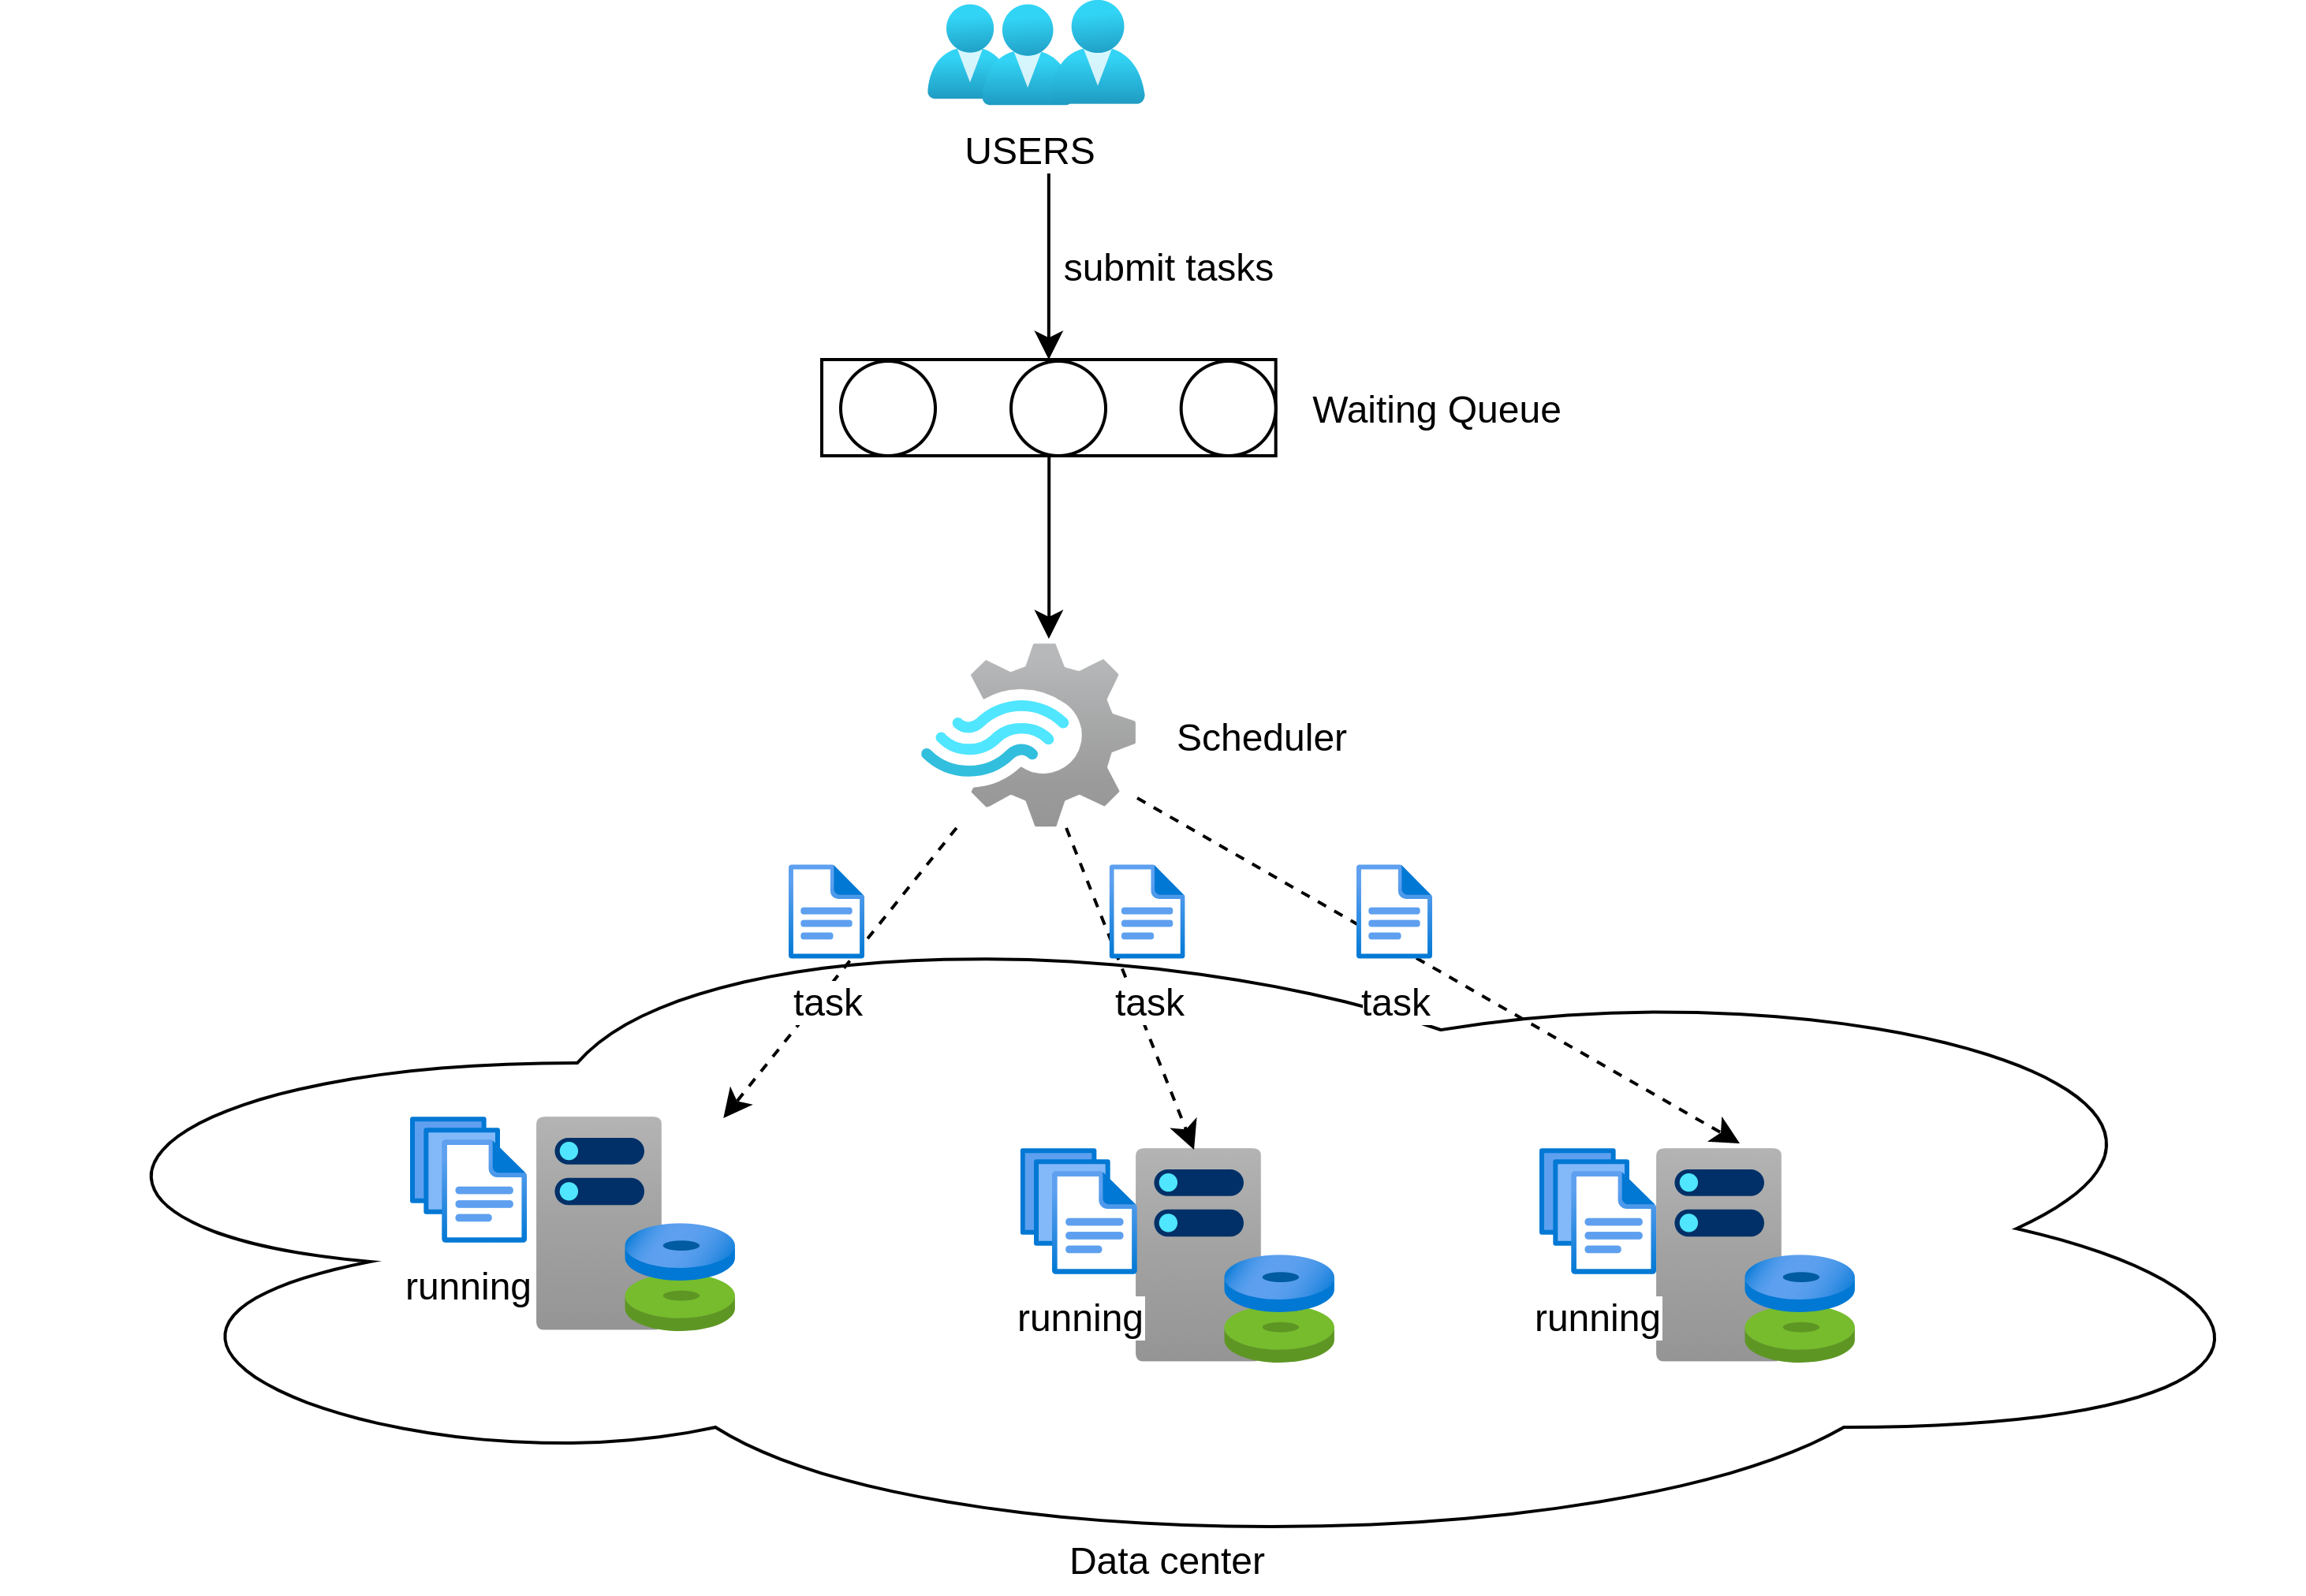
\includegraphics[width=8cm]{images/basic_flow.png} }}%
    \qquad
    \subfloat[\centering Trạng thái của task]{{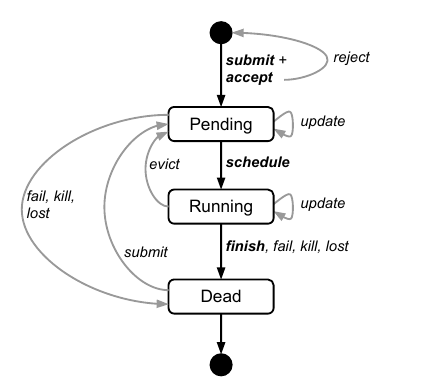
\includegraphics[width=5cm]{images/task_states.png} }}%
    \caption{Luồng di chuyển của task}%
    \label{fig:flow}%
\end{figure}
Với các giải thuật lập lịch có sẵn, có 2 vấn đề chưa được khắc phục trong mô hình thực tế, đó là sự sai lệch về các thông số do độ trễ của hệ thống, và sự mất tính load-balancing khi các công việc batch-job kết thúc còn các công việc long-running vẫn đang chạy tập trung trên một vài máy ảo. 

\subsection{Sai lệch về thông tin do độ trễ của hệ thống}
Có thể thấy rằng trong khi chạy, task có thể bị fail và được đưa trở về hàng đợi đến lần lập lịch tiếp theo, hoặc cũng có thể kết thúc và rời khỏi máy tính ảo. Mỗi khi điều này xảy ra, tài nguyên của hệ thống được giải phóng và có thể phân phối cho các tasks khác. Điều này khiến cho thông tin môi trường sẽ thay đổi liên tục trong khi hoạt động. Như vậy, các thông số của hệ thống mà được sử dụng trong quá trình lập lịch có thể không thống nhất với thời điểm chạy, khiến cho nghiệm tối ưu của bài toán lập lịch không tốt như mong muốn trong quá trình chạy.\\
\begin{figure}[h!]
	\centering
	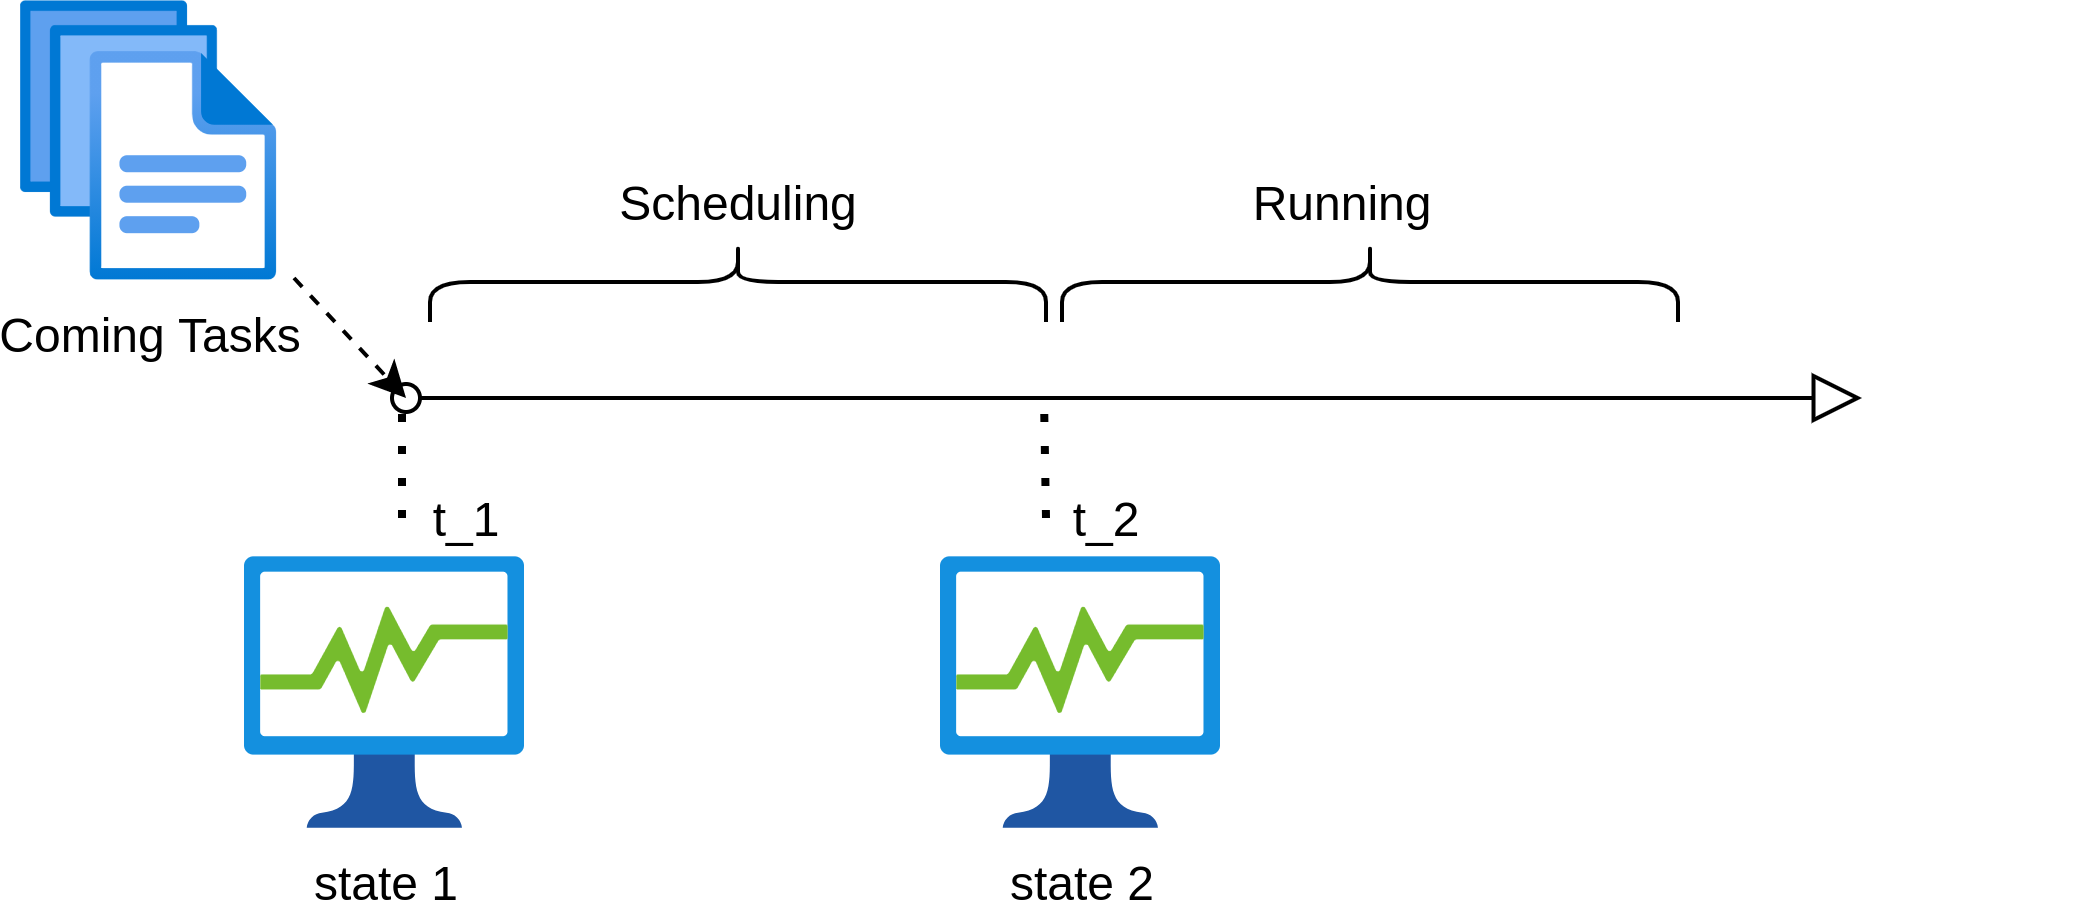
\includegraphics[scale=0.8]{images/state_change.png}
	\caption{Trạng thái máy tính tại thời điểm lập lịch và thực thi}
	\label{fig:statechange}
\end{figure}

\noindent
Cụ thể hơn, xét tại thời điểm $t_{1}$, các tasks trong hàng đợi được mang ra lập lịch, scheduler sẽ lấy các thông số của hệ thống tại thời điểm đó là $state_{1}$. Quá trình lập lịch trong môi trường phân tán cần lấy thông tin từ các thành phần khác nhau, chạy thuật toán và phân phối tasks đến các máy ảo tương ứng. Điều này khiến cho thời điểm các tasks bắt đầu được thực thi trên máy ảo là $t_{2}$ sẽ trễ hơn so với thời điểm $t_{1}$ một lượng $\delta_{t}$ đáng kể (hình ~\ref{fig:statechange}). Như vậy, trong thời gian lập lịch thì các task đang chạy trong các máy ảo có thể được hoàn thành, bị fail hoặc bị hoãn, dẫn đến khả năng $state_{2} \neq state_{1}$. Mà quyết định lập lịch là nghiệm bài toán tối ưu thu được dựa trên thông số $state_{1}$ nên sự chênh lệch này sẽ phá vỡ tính tối ưu của thuật toán lập lịch. 
\subsection{Mất cân bằng tải}
\label{unload_balancing}
Với các tasks được gửi từ người dùng, ví dụ như trong hệ thống máy chủ của Google\cite{18}, không thể xác định được execution time với các thông tin tại thời điểm lập lịch. Do đó, các thuật toán lập lịch quan tâm chính đến vấn đề tài nguyên khả dụng, mà chưa xem xét đến thời điểm kết thúc của tasks. Điều này có thể gây ra sự mất cân bằng load-balancing trong quá trình hoạt động. Trong hình ~\ref{fig:unload_balancing}, các tasks thuộc dạng batch-job kết thúc trước khiến cho trạng thái load-balancing của hệ thống bị phá vỡ. 
\begin{figure}
	\centering
	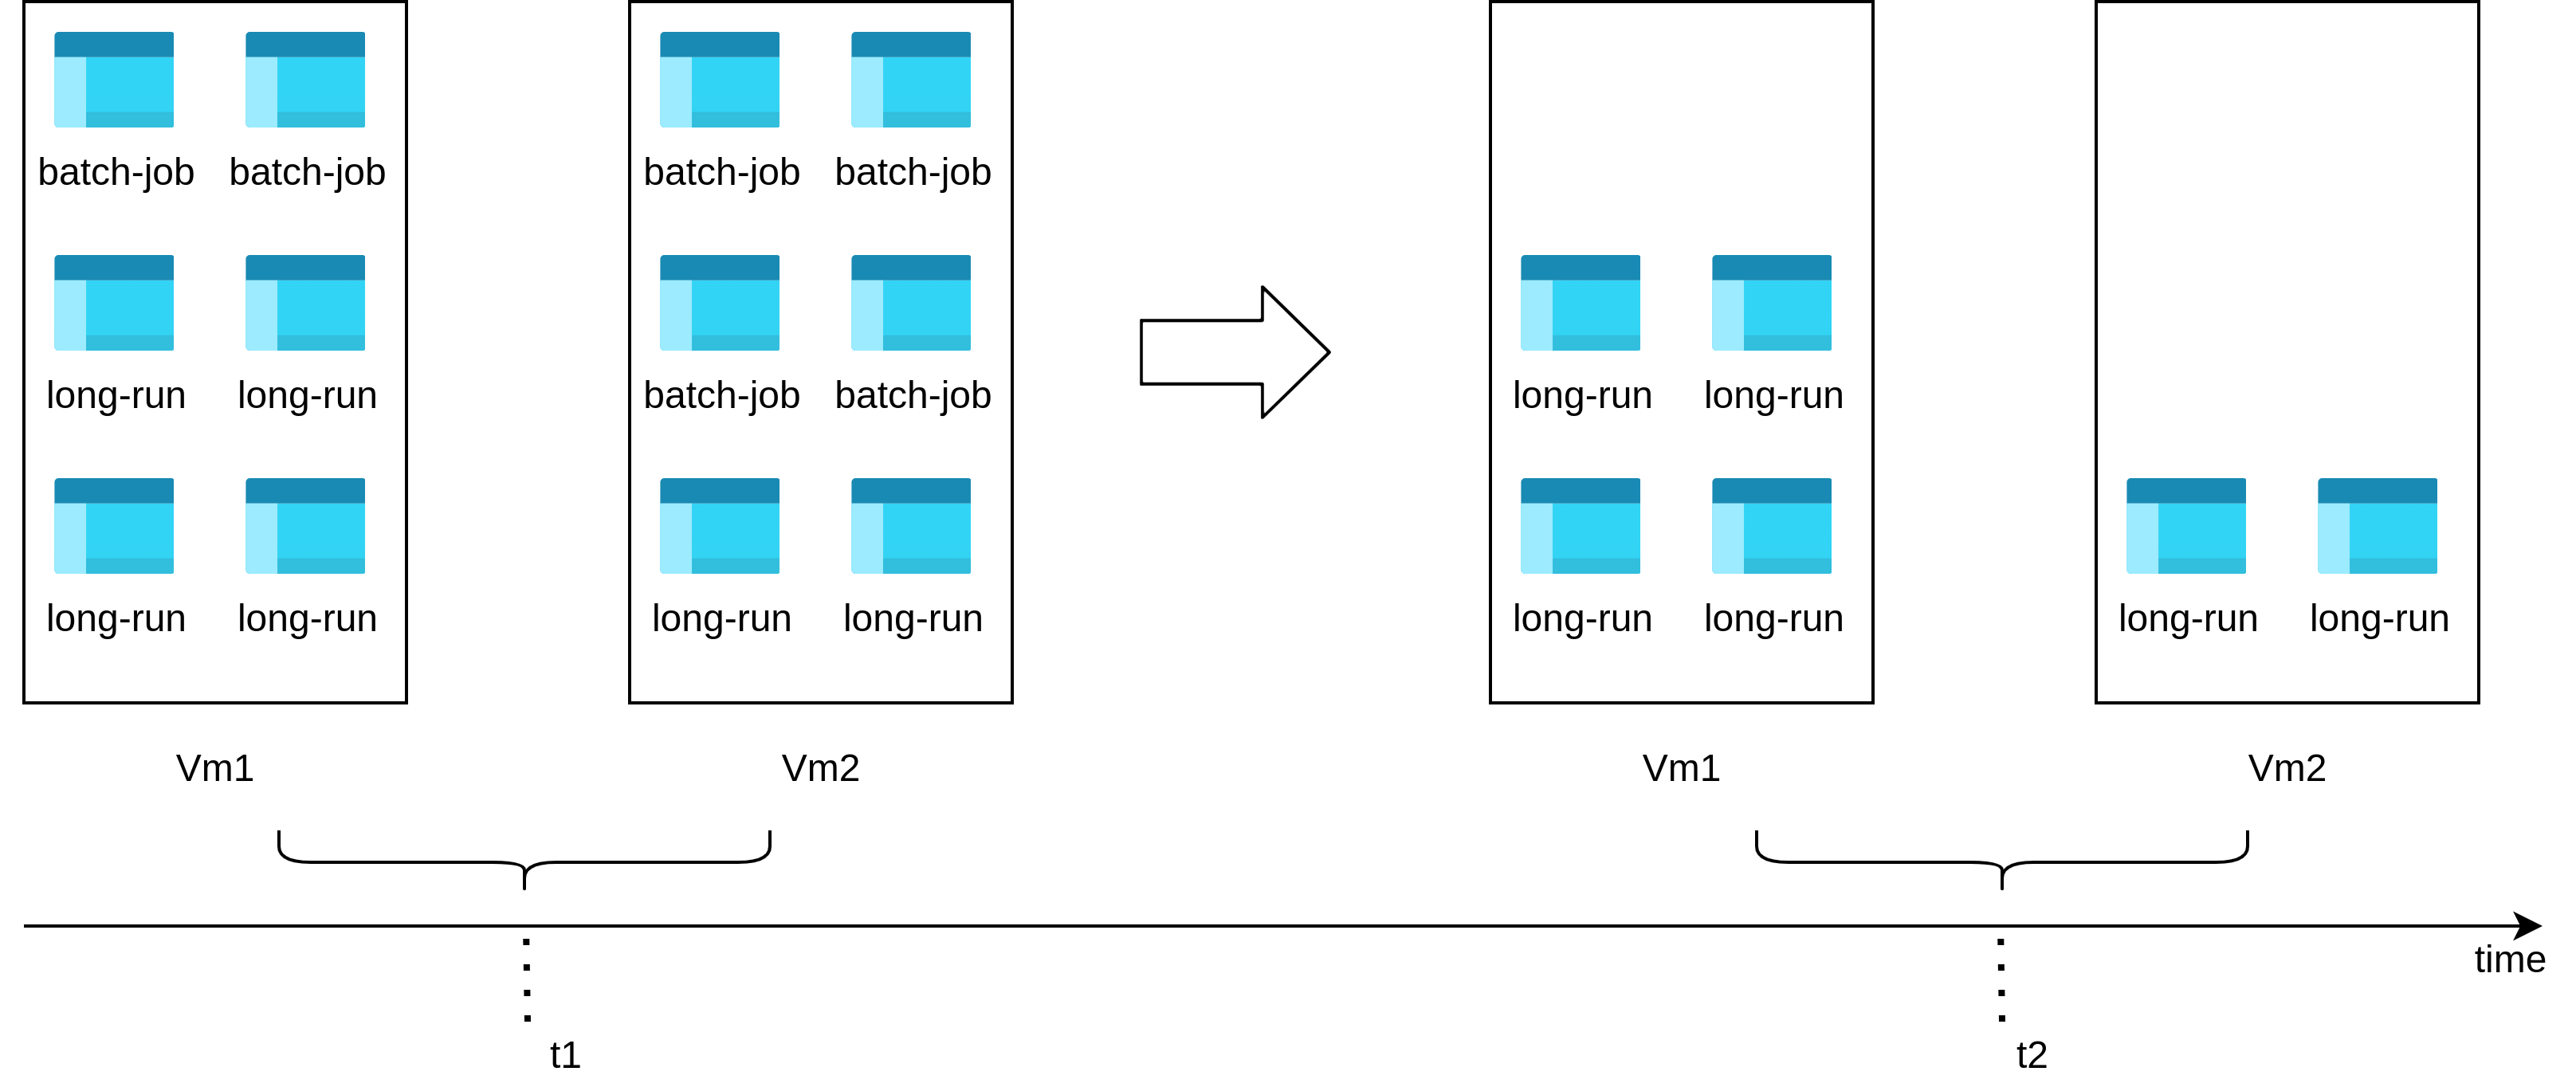
\includegraphics[scale=0.5]{images/unload_balancing.png}
	\caption{Mất cân bằng giữa các task do sự kết thúc của batch-job tasks}
	\label{fig:unload_balancing}
\end{figure}

\section{Mô hình đề xuất}
$\mathcal{V}$ là tập máy ảo trong hệ thống, $\mathcal{V} = \{vm_{1}, vm_{2}, ..., vm_{M}\}$, với 
\[
vm_{i}.v = [v_{i}^{1}, v_{i}^{2}, v_{i}^{3}, v_{i}^{4}]
\]
là vector mang thông tin tài nguyên của máy ảo, lần lượt là cpu, bộ nhớ chính, băng thông mạng và ổ đĩa. Task đên hệ thống sẽ gồm những thông tin sau: 
\begin{enumerate}
	\item $c = [c^{1}, c^{2}, c^{3}, c^{4}]$ là vector tài nguyên task yêu cầu, lần lượt là cpu, bộ nhớ chính, băng thông mạng và ổ đĩa
	\item meta\_data bao gồm thông tin về người dùng, application gửi task đến, mức độ ưu tiên
	\item lib: rằng buộc về thư viện, môi trường thực thi 
\end{enumerate}

Lập lịch là công việc tìm hàm ghép cặp task với máy ảo 
\[
f: \mathcal{C} \rightarrow \mathcal{V}
\]
với $\mathcal{C}$ là không gian các tasks.\\
Với mỗi máy tính ảo $vm_{i}$, $r_{i} = \{task_{i1}, ..., task_{ik}\}$ là tập các tasks đang được chạy trong nó. Trong khi lập lịch, ta cần đảm bảo được điều kiện tài nguyên của máy tính phải lớn hơn tổng nhu cầu sử dụng của các tasks: 
\[
	vm_{i}.v \geq \sum_{j = 1}^{k}task_{ij}.c
\]
Trong trường hợp tài nguyên không đủ, các tasks có mức ưu tiên thấp hơn sẽ bị dừng lại hoặc hủy và trả về hàng đợi để nhường tài nguyên cho các tasks còn lại. 
\begin{figure}
	\centering
	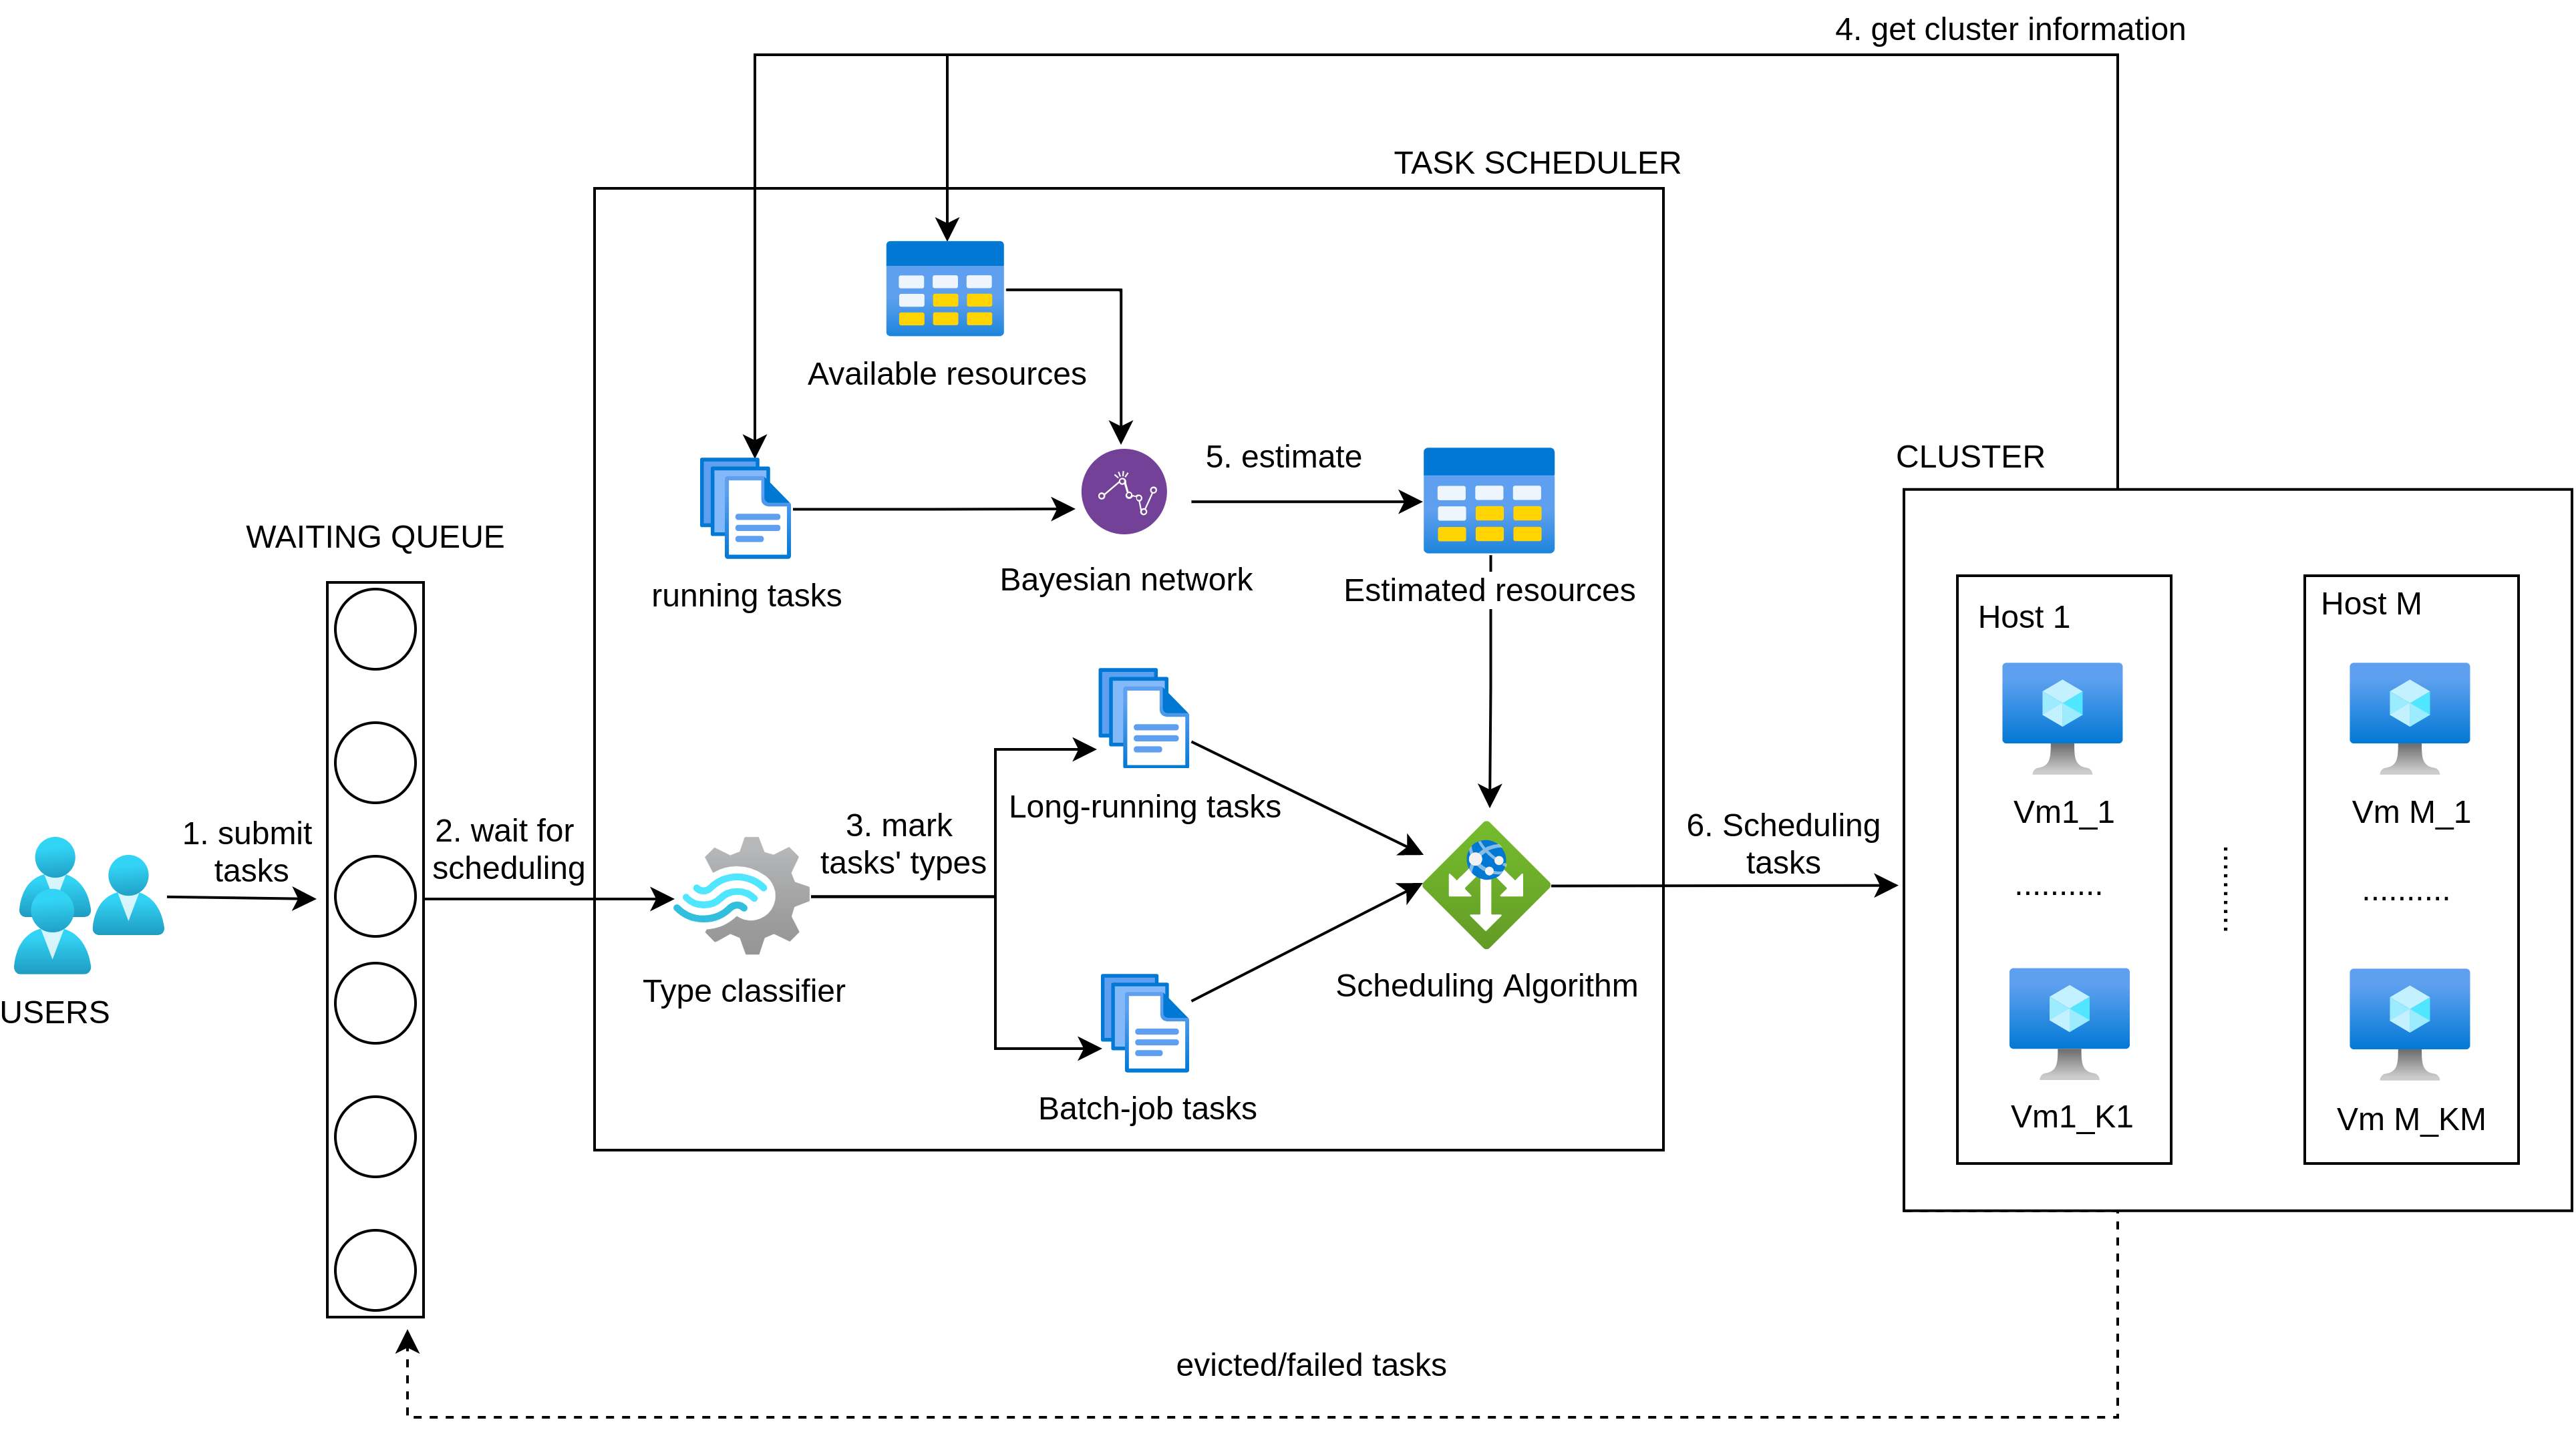
\includegraphics[scale=0.5, height=7cm]{images/system_flows.png}
	\caption{Mô hình lập lịch}
	\label{fig:systemflow}
\end{figure}
Hình ~\ref{fig:systemflow} là mô hình một lịch được đề xuất, bao gồm: 
\begin{enumerate}
	\item Người dùng gửi các công việc đến hệ thống, được chuyển đến hàng đợi cho việc lập lịch
	\item Các tasks chờ đợi đến khi đủ số lượng hoặc vượt quá một khoảng thời gian cố định 
	\item Dựa vào thông tin metadata của tasks, ta phân loại công việc thành 2 kiểu là long-running và batch-job
	\item Bộ lập lịch lấy các thông tin về trạng thái hệ thống, bao gồm các tasks đang được chạy trong hệ thống và thông tin về tài nguyên của các máy tính ảo 
	\item Sử dụng mạng Bayesian để ước lượng tài nguyên khả dụng tại thời điểm tasks được thực thi trên các máy ảo 
	\item Lập lịch cho các tasks với thông tin tài nguyên ước lượng
\end{enumerate}

\subsection*{Phân loại tasks}
Việc nhận đinh một task thuộc dạng long-running hay batch-job không phải là dễ dàng. Điều quyết định đến thời gian chạy của công việc là người dùng, họ có thể dừng các dịch vụ một cách tùy ý họ muốn, nên đôi khi long-running chưa hẳn thời gian hoạt động đã đủ "long" (dài). Mặc dù vậy, trong \cite{17}, tác giả sử dụng thông tin về ứng dụng mà gửi task đến hệ thống để phân loại. Các tasks được gửi từ Gmail, Google Docs, Google Slide, ... sẽ được xem là long-running. Còn với những tasks từ Google Data Analytic, Google Auto ML, ... thì là batch-jobs.  Việc phân chia như vậy là dựa vào đặc thù từng ứng dụng, các ứng dụng long-running sẽ là các application tương tác liên tục với người dùng, còn batch-job thì sau khi gửi công việc thì sẽ ko cần tương tác cho đến khi kết thúc.

\subsection{Dự đoán tài nguyên khả dụng}
Với các thuật toán trước đó, ta mặc định $state_{2} = state_{1}$ (hình ~\ref{fig:statechange}), tức là các tasks đang chạy trong các máy ảo sẽ không thay đổi trạng thái trong quá trình lập lịch. Nhưng trong thực tế không phải như vậy, việc lập lịch kéo dài tới vài giây, hoặc vài phút, tùy theo số lượng tasks và tốc độ truyền tin trong mạng. Một batch-job task có thời gian từ vài giây đến vài ngày \cite{17}\cite{18}, như vậy việc tasks đang chạy trong hệ thống thay đổi trạng thái trong giai đoạn lập lịch làm $state_{2} \neq state_{1}$ xảy ra rất thường xuyên. Như đã đề cập ở đầu chương, việc sai lệch thông tin này khiến cho lời giải của thuật toán không còn tối ưu như kỳ vọng. \\
Từ giờ, ta sẽ gọi các tasks đang chạy trong các máy ảo là running-tasks, các tasks đang ở hàng đợi là waiting-tasks. Mục tiêu của ta là ước lượng trạng thái của các running-tasks tại thời điểm các waiting-tasks bắt đầu được thực thi ($t_{2}$ trong hình ~\ref{fig:statechange}), và từ đó ước lượng số lượng tài nguyên khả dụng của hệ thống để phục vụ cho việc lập lịch tại $t_{1}$. \\
Phương pháp ước lượng được đề xuất là sử dụng mô hình Bayesian tìm mối quan hệ giữa các tasks thuộc cùng một job để đưa ra phán đoán về trạng thái. 
\begin{figure}[h!]
	\centering 
	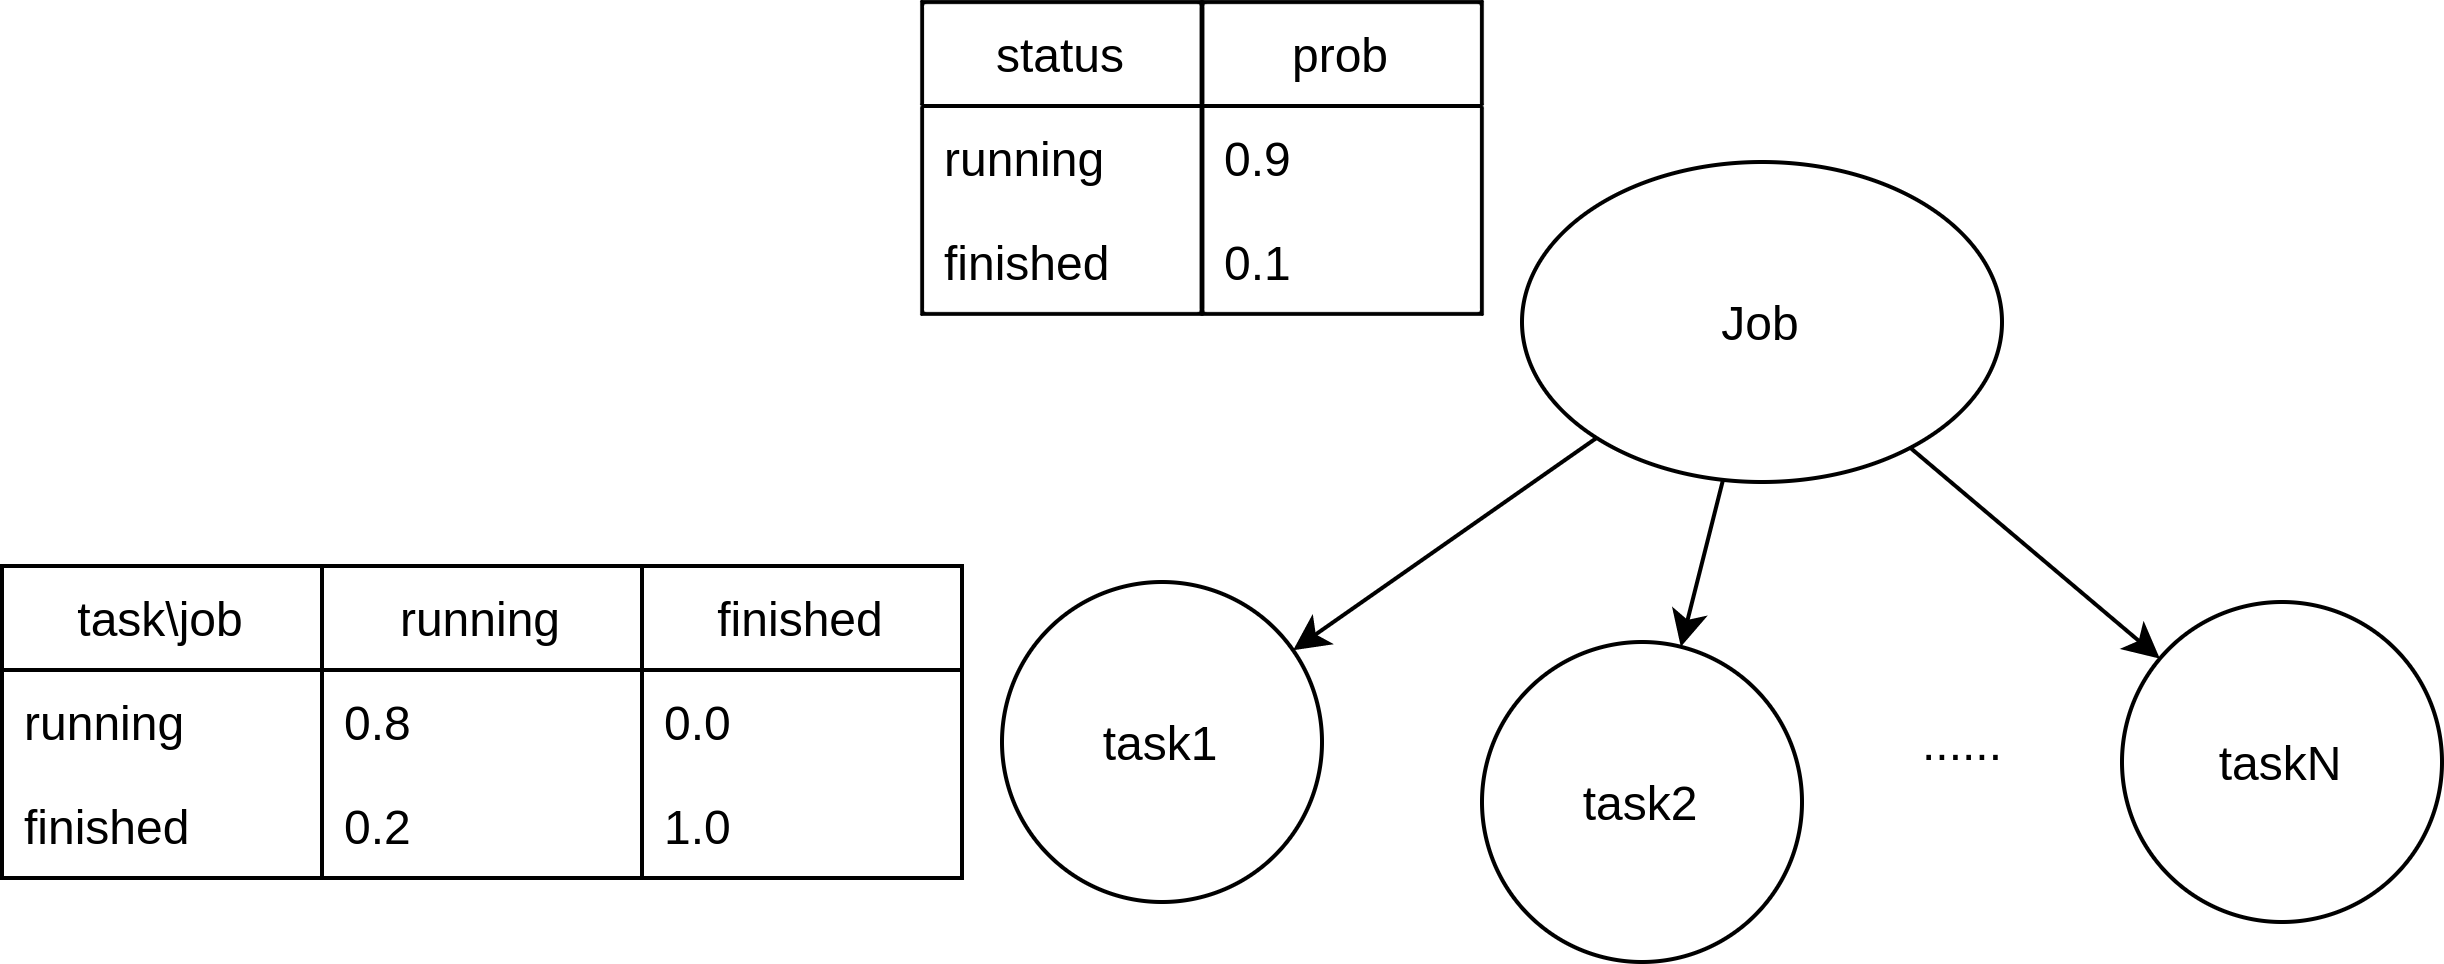
\includegraphics[scale=0.6]{images/job_network.png}
	\caption{Mạng Bayesian thể hiện quan hệ giữa các tasks trong cùng một job}
	\label{fig:job_network}
\end{figure}
Trong hình ~\ref{fig:job_network}, trạng thái mỗi task là một biến ngẫu nhiên được biểu thị bởi một đỉnh trong đồ thị, với tập giá trị là running (trong trường hợp task đang được thực thi) và finished (trong trường hợp tài nguyên dành cho task được thu hồi). Các tasks trong cùng một job đều phụ thuộc vào job như trong hình \ref{fig:job_network}. Trong bảng phân phối xác suất của task, con số 0.8 ý nghĩa
\[
 P(task = running \mid job = running) = 0.8
\]
là xác suất task đang chạy khi biết job vẫn đang chạy. \\
Với đồ thị trên, ta có: 
\begin{align*}
	P(task) &= \sum_{s \in \{running, finished\}}P(task, job = s) \\
			&= \sum_{s \in \{running, finished\}}P(job = s)P(task \mid job = s)
\end{align*}

\noindent
Từ đó, ta tính được P(task = running) = 0.72 và P(task = finished) = 0.28. \\
Sau đây, ta sẽ mô tả cách thức chúng ta dùng đồ thị Bayesian để suy diễn trạng thái của các tasks. Xét với trường hợp job có 2 tasks như hình ~\ref{fig:two_tasks}. \\
\begin{figure}[h!]
	\centering
	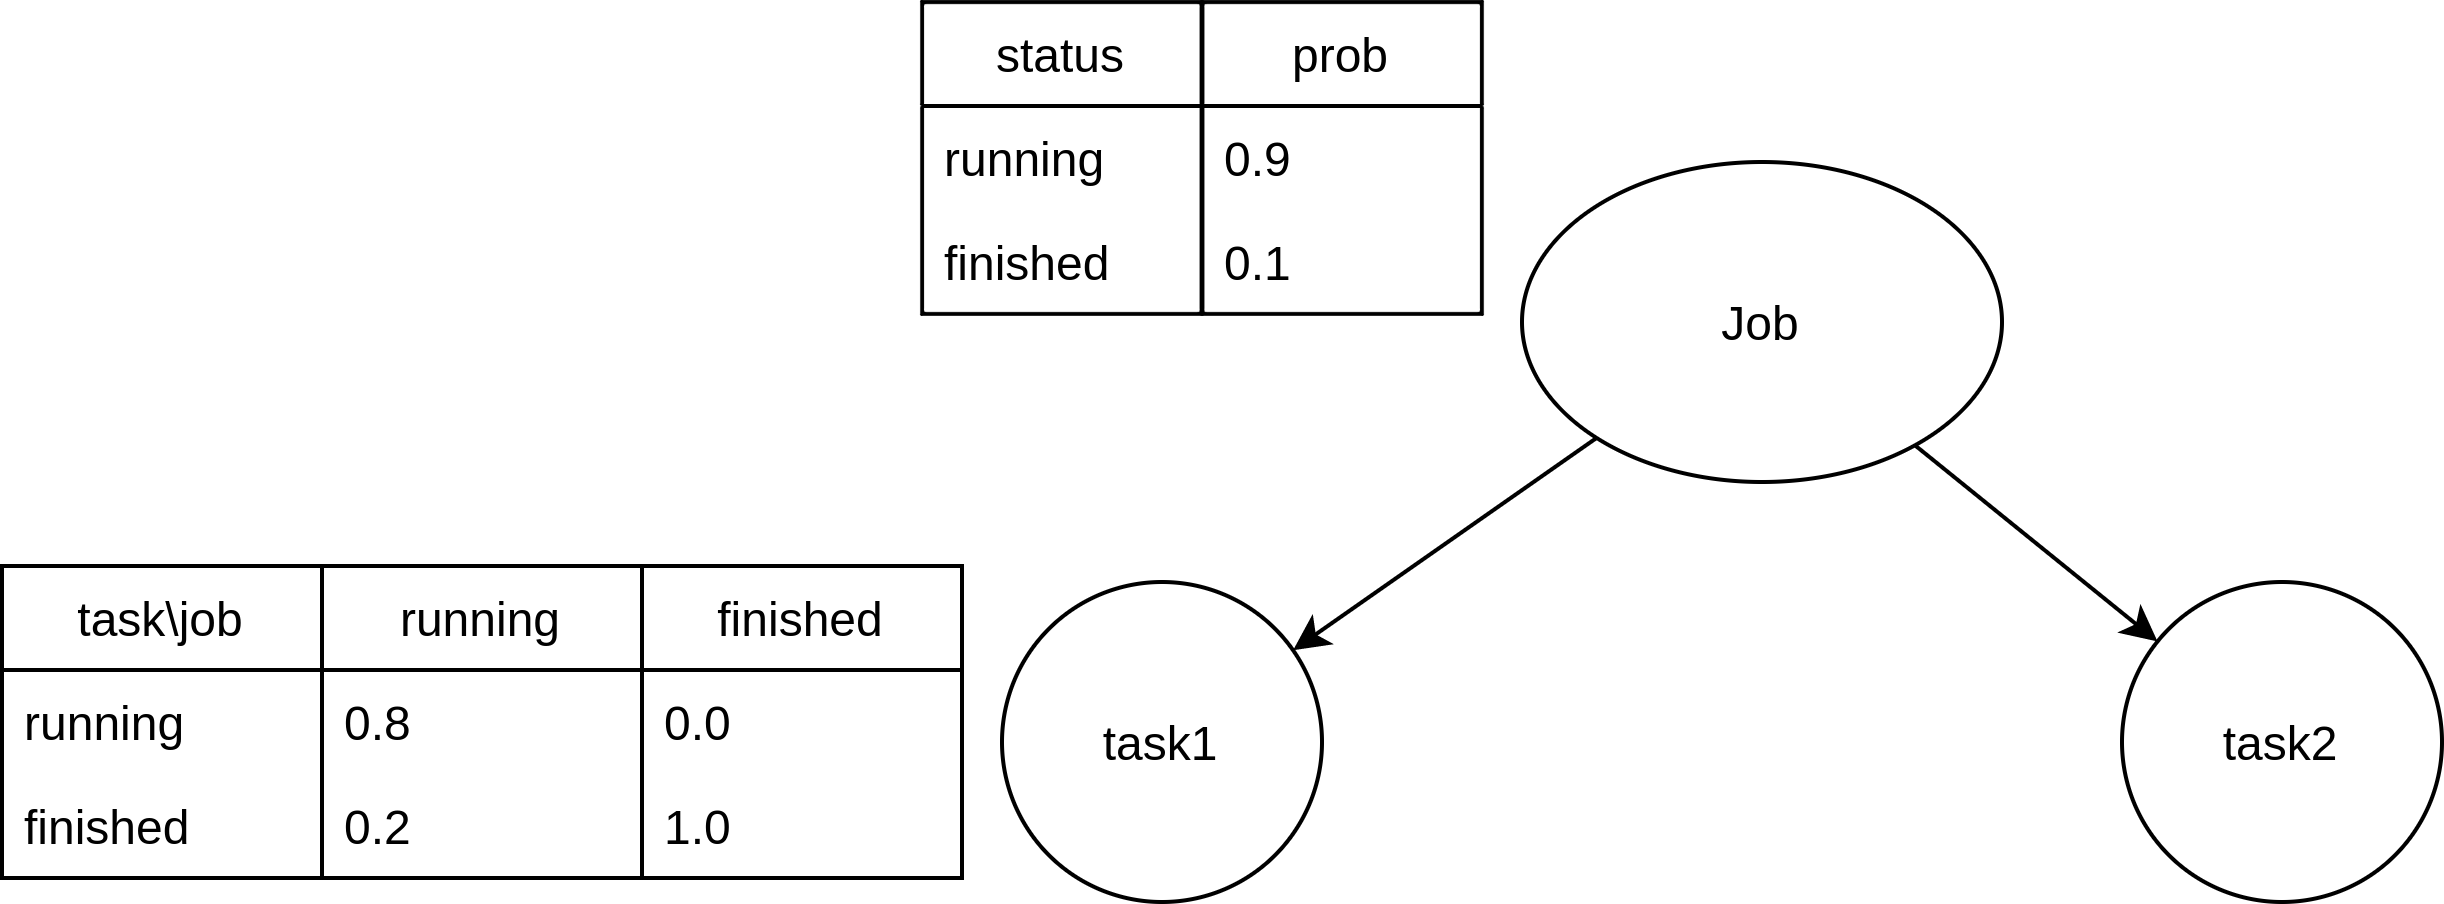
\includegraphics[scale=0.6]{images/two_tasks.png}
	\caption{Mạng Bayesian cho trường hợp có 2 tasks}
	\label{fig:two_tasks}
\end{figure}

\noindent
Giả sử ta quan sát được task1 đã kết thúc, tức là trạng thái của nó là finished, khi đó phân phối xác suất của task2 sẽ như thế nào?\\
 Ta sẽ tính 
\begin{align*}
	P(task2 \mid task1 = finished) &= \sum_{job}P(task2, job \mid task1 = finished) \\
									&= \sum_{job}\frac{P(task2, job, task1 = finished)}{P(task1 = finished)} \\
\end{align*}
Trong đồ thị Bayesian~\ref{fig:two_tasks}, ta phân tích được: 
\[
	P(task2, job, task1) = P(job) \times P(task1 \mid job) \times P(task2 \mid job)
\]
Suy ra, 
\begin{align*}
	P(task2 \mid task1 = finished) &= \sum_{job}\frac{P(job)P(task2 \mid job) \times P(task1 = finished \mid job)}{P(job) \times P(task1 = finished \mid job)}
\end{align*}
Thay các giá trị vào, tính được: 
\begin{align*}
	&P(task2 = running \mid task1 = finished) = 0.514 \\
	&P(task2 = finished \mid task1 = finished) = 0.486 \\
\end{align*}
Chú ý rằng bởi vì quan sát được task1 kết thúc mà xác suất để task2 kết thúc tăng từ 0.28 lên thành 0.486, phù hợp với thực tế rằng khi có một task kết thúc các task còn lại trong job tăng khả năng kết thúc sau đó. \\
Như vậy, làm thế nào để có được P(task | job) và P(job) tại một thời điểm ngẫu nhiên trong quá trình chạy. Trong đồ án này, ta ghi lại các trạng thái của các thành phần trong hệ thống tại thời điểm đầu lập lịch và kết thúc lập lịch, sau đó tính tỉ lệ giữa các trạng thái. Ta đã biết với phân phối xác suất dạng bảng như trên thì tỉ lệ giữa các giá trị quan sát của biến ngẫu nhiên chính là nghiệm của hàm tối ưu likelihood trên bộ dữ liệu (trang 719, \cite{28}). \\
\begin{figure}[h!]
	\centering
	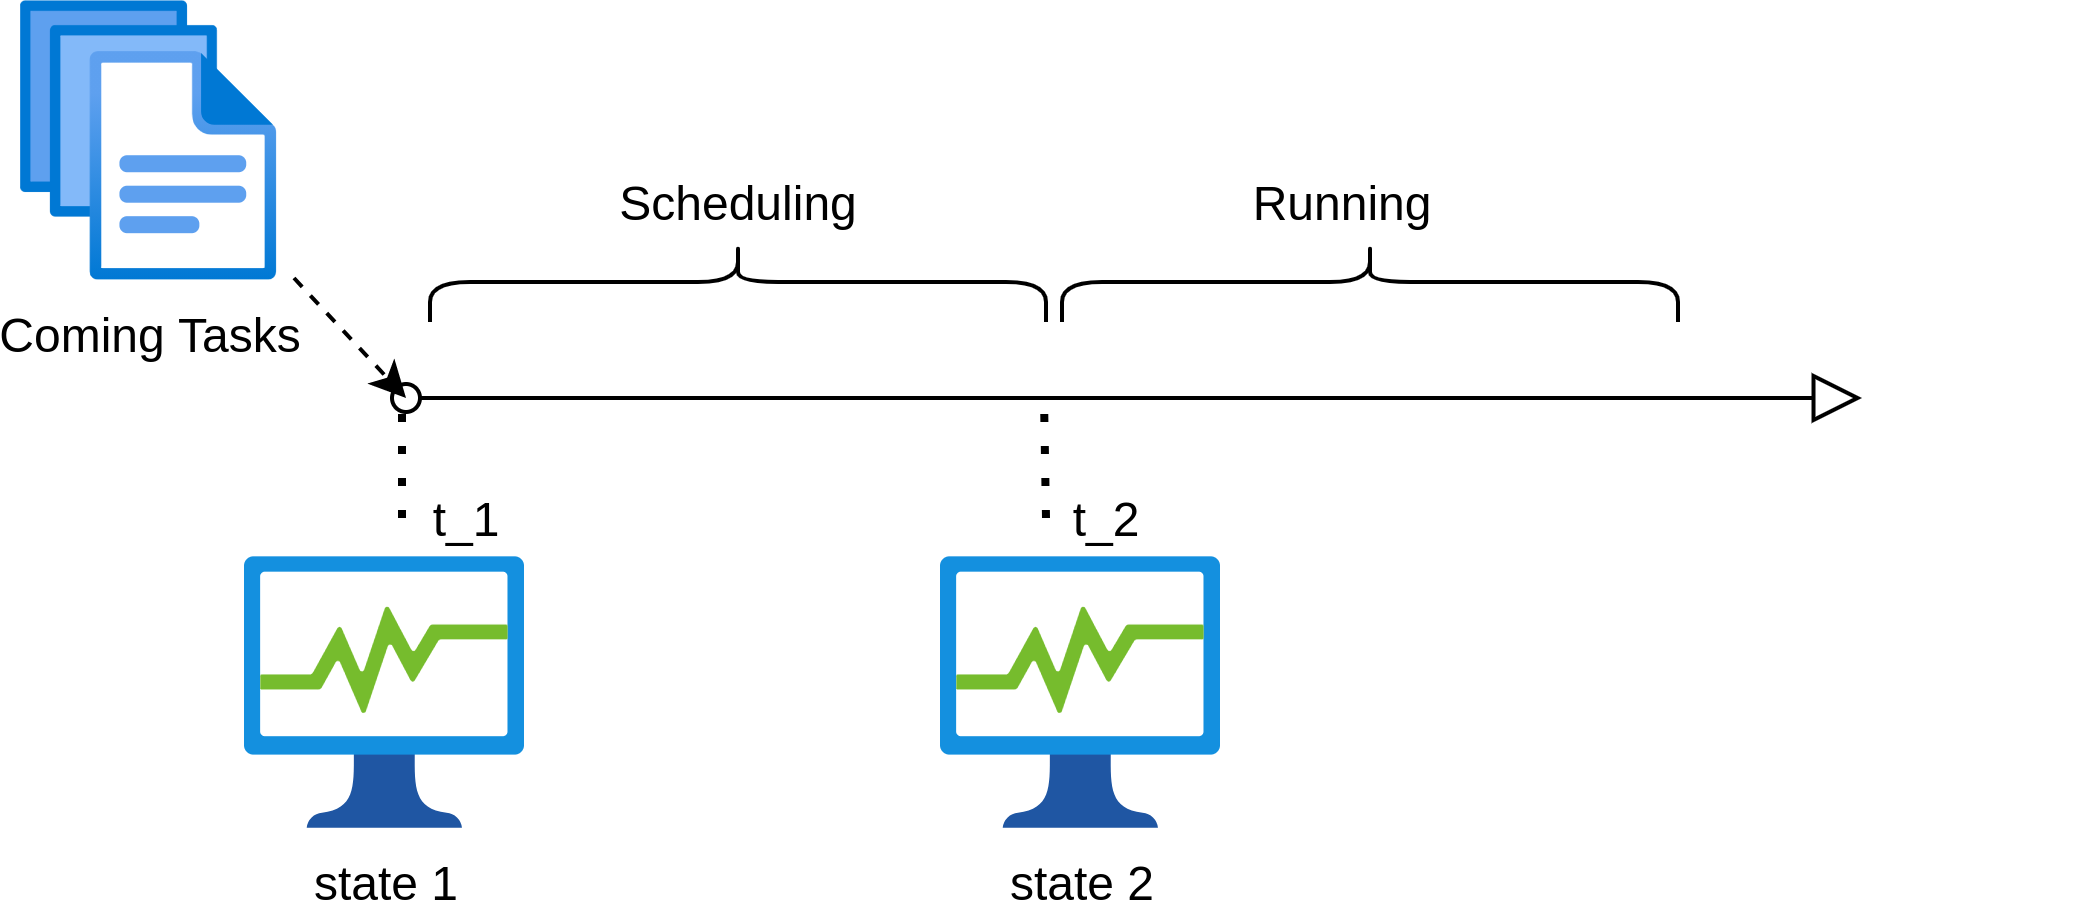
\includegraphics[scale=0.8]{images/state_change.png}
	\caption{Trạng thái máy tính tại thời điểm lập lịch và thực thi}
	\label{fig:statechange1}
\end{figure}

\noindent
Trong hình ~\ref{fig:statechange1}, tại thời điểm $t_{1}$ khi bắt đầu lập lịch, ta sẽ ước lượng trạng thái tài nguyên (đã dùng và chưa sử dụng) tại thời điểm kết thúc lập lịch khi mà các tasks được thực thi trên các máy ảo, $t_{2}$. Cụ thể, ta sẽ tính kỳ vọng của tài nguyên được sử dụng của từng máy ảo tại thời điểm $t_{2}$. 
\begin{algorithm}[H]
\textbf{Input:} $vms: List<vm>$ \\ 
\textbf{Output:} $List<vector>$ - list với phần tử là vector tài nguyên khả dụng của các máy ảo
\begin{algorithmic}[1]
	\STATE$ availables \leftarrow  List<vector>$
	\FOR{$vm \in vms$}
		\STATE $remainder \leftarrow vm.v$
		\FOR{$task \in vm.runningTasks$}
			\STATE $prob \leftarrow BayesianNetwork.\textbf{inference}(task)$
			\STATE $remainder \leftarrow remainder - prob \times task.c$
		\ENDFOR
		\STATE $availables.add(remainder)$
	\ENDFOR
	\RETURN $availables$
\end{algorithmic}
\caption{Estimate usage of vms }
\label{alg:1}
\end{algorithm}

\noindent
Trong thuật toán~\ref{alg:1}, ở dòng số 5, ta dùng thuật toán Belief Propagation~\cite{29} trên mạng Bayesian để ước lượng P(task is running at $t_{2}$), và kỳ vọng tài nguyên sử dụng sẽ là xác suất task còn đang chạy (tức còn chiếm tài nguyên) nhân với tài nguyên task sử dụng. Nên nhớ rằng công việc ước lượng này là một phần của thuật toán lập lịch, nên thời gian chênh lệch 
\[
	\delta_{t} = t_{2} - t_{1} = time_{inference} + time_{matching} + network\_delay
\]
có thể ước lượng được. 
Trong những trường hợp thời gian chênh lệch không đáng kể, $\delta_{t} < \epsilon$, ví dụ như số lượng task cần được lập lịch rất ít, ta sẽ không thực hiện ước lượng vì sự sai lệch không đáng kể.

\subsection{Thuật toán lập lịch đề xuất}
\label{proposed_algo}
Sau khi ước lượng được tài nguyên khả dụng của hệ thống tại thời điểm kết thúc lập lịch, ta cần ghép cặp giữa tasks và máy ảo. Mục tiêu của thuật toán ghép cặp là ổn định tính load-balancing trong quá trình chạy, giải quyết vấn đề được đưa ra trong mục~\ref{unload_balancing}. Ý tưởng tiếp cận là ta sẽ cố gắng cân bằng tài nguyên sử dụng giữa các máy ảo và cân bằng lượng tài nguyên phân phối cho batch-job giữa các máy ảo.\\
Trước tiên, ta đề xuất thuật toán cân bằng khối lượng công việc giữa các máy ảo~\ref{alg:2}. Xét 
\[
	\mathcal{L} = \{l_{1}, l_{2}, ..., l_{M}\}
\]
là tập biểu diễn khối lượng công việc của M máy ảo. Ta coi độ mất cân bằng của hệ thống chính là phương sai tập $\mathcal{L}$: 
\[
	\sigma(\mathcal{L}) = \frac{1}{M} \times \sum_{i = 1}^{M}(l_{i} - \overline{l})^{2}
\]
với 
\[
	\overline{l} = \frac{1}{M}\sum_{i = 1}^{M}l_{i}
\]
Đầu vào của thuật toán sẽ là tập các tasks với khối lượng công việc $\mathcal{C} = \{c_{1}, ..., c_{N}\}$, ta sẽ đưa ra cách phân phối chúng đến máy ảo sao cho sự mất cân bằng của hệ thống là nhỏ nhất. Trọng số của một cách ghép cặp $task_{i} \rightarrow vm_{j}$ là chênh lệch của $\sigma(\mathcal{L})$ trước và sau khi ghép cặp.
\[
	\Delta_{L}(task_{i} \rightarrow vm_{j}) = \frac{1}{M}[(l_{j} + c_{i} - \overline{l^{'}})^{2} - (l_{i} - \overline{l})^{2}]
\]
với 
\[
	\overline{l^{'}} = \frac{1}{M}(\sum_{k = 1}^{M}l_{k} + c_{i})
\]
Trong thuật toán~\ref{alg:2}, ta thực hiện vòng lập đến khi tất cả các tasks đều được lập lịch. Trong mỗi vòng lặp, ta sẽ tính ma trận $\Delta$, với $\Delta_{ij}$ là trọng số của cách ghép $task_{i} \rightarrow vm_{j}$ (dòng 3). Ta thực hiện gán cặp task, máy tính ảo sao độ mất cân bằng là nhỏ nhất, sau đó sẽ tăng thêm giá trị khối lượng công việc cho cái máy tính vừa được lập lịch. Đây là một thuật toán heuristic, với độ phức tạp là $O(MN^{2})$ do sau mỗi lần ghép cặp thì trong số của tất cả các phép gán tiếp theo sẽ bị thay đổi, nên ta lại phải cập nhật lại. \\
\begin{algorithm}[H]
\textbf{Input:} \\
$\mathcal{L} = \{l_{1}, l_{2}, ..., l_{M}\}$\\
$\mathcal{C} = \{c_{1}, ..., c_{N}\}$ \\ 
\textbf{Output:} \\
Cách ghép cặp cho task với vm
\begin{algorithmic}[1]
	\STATE $solution = \{\}$
	\WHILE{$|solution| \neq N$}
		\STATE $\Delta \leftarrow \textbf{calculate\_unbalanced\_factor}(\mathcal{L}, \mathcal{C})$
		\STATE $(i, j) = argmin(\Delta)$
		\STATE $solution \rightarrow solution \cup (task_{i} \rightarrow vm_{j})$
		\STATE $C \leftarrow C \setminus \{c_{i}\}$
		\STATE $l_{j} \leftarrow l_{j} + c_{i}$
	\ENDWHILE
	\RETURN $solution$
\end{algorithmic}
\caption{Load-balancing scheduling algorithm}
\label{alg:2}
\end{algorithm}

\noindent
Quay trở lại bài toán lập lịch thời gian thực, với máy ảo $vm_{i}$, vector $vm_{i}.v = [v_{i}^{1}, v_{i}^{2}, v_{i}^{3}, v_{i}^{4}]$ biểu diễn tài nguyên của máy tính, $r_{i} = \{task_{i1}, ..., task_{ik}\}$ là tập các tasks đang được chạy trong nó.\\
Với $task_{ij}$, 
\[
task_{ij}.type = 
	\begin{cases}
		\text{0, } &\quad\text{nếu $task_{ij}$ thuộc kiểu long-running} \\
		\text{1, } &\quad\text{nếu $task_{ij}$ thuộc kiểu batch-job}
	\end{cases}
\]
Ta xem xét tài nguyên đã được sử dụng là tổng của những phần dành cho long-running tasks với những phần dành cho batch-job tasks. Dựa vào thuật toán ~\ref{alg:1}, ta tính kỳ vọng lượng tài nguyên mà các batch-job tasks sử dụng tại thời điểm kết thúc lập lịch là: 
\[
	vm_{i}.EshortUsage = \sum_{j=1}^{k}task_{ij}.c \times task_{ij}.type \times prob_{task_{ij}}
\]

\noindent
$vm_{i}.longUsage$ là tài nguyên của máy ảo dành cho long-running tasks.
\[
	vm_{i}.longUsage = \sum_{j = 1}^{k}task_{ij}.c \times (1 - task_{ij}.type)
\]
$vm_{i}.usage$ là tài nguyên được sử dụng tại thời điểm kết thúc lập lịch, 
\[
	vm_{i}.Eusage = vm_{i}.EshortUsage + vm_{i}.longUsage
\]
Ta tính được 2 tập hợp biểu diễn khối lượng công việc giữa các máy tính ảo: 
\begin{itemize}
	\item $\mathcal{L}_{batch} = \{vm_{1}.EshortUsage, ..., vm_{M}.EshortUsage\}$ là tập khối lượng tài nguyên được sử dụng bởi batch-job tasks 
	\item $\mathcal{L} = \{vm_{1}.Eusage, ..., vm_{M}.Eusage\}$ là tập khối lượng toàn bộ tài nguyên được sử dụng
\end{itemize}
\begin{figure}[h!]
	\centering
	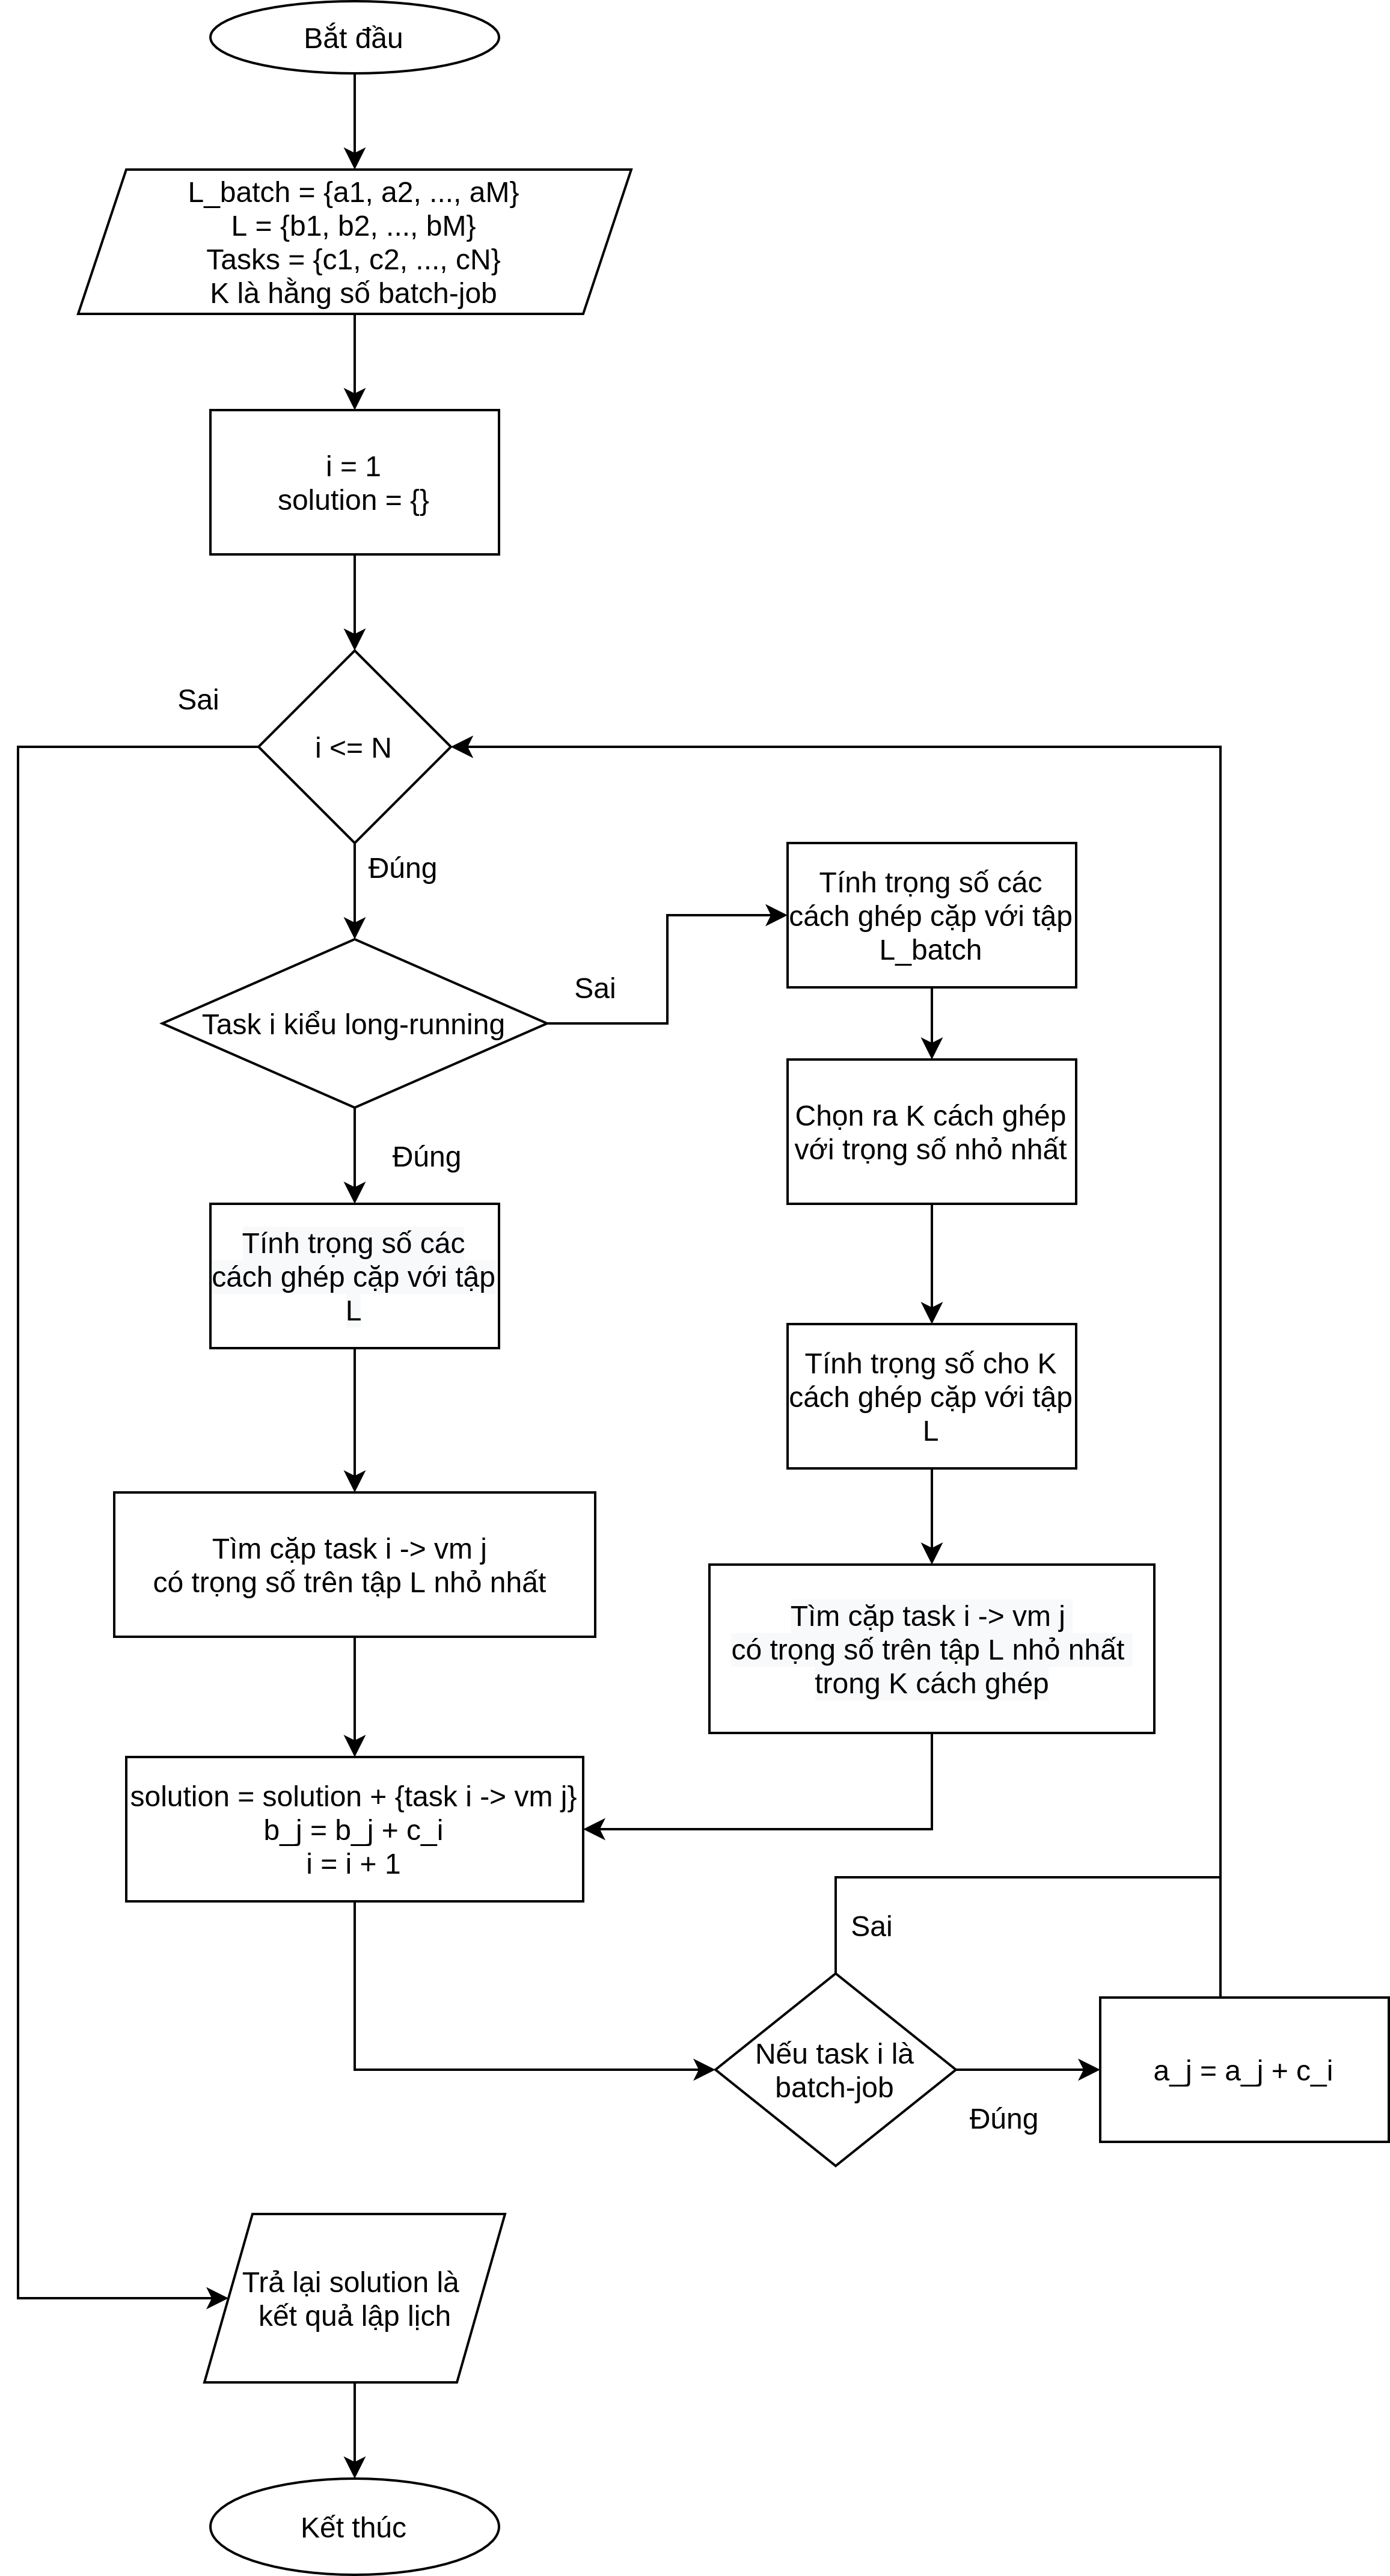
\includegraphics[scale=0.7]{images/load_balancing_proposal.png}
	\caption{Thuật toán lập lịch cân bằng giữa long-running và batch-job}
	\label{fig:algo3}
\end{figure}
Thuật toán đề xuất được mô tả trong hình ~\ref{fig:algo3}, hướng tới việc cân bằng lượng tài nguyên phân phối cho batch-job, đồng thời cân bằng tổng lượng tài nguyên giữa các máy ảo, được mô tả như sau: 
Các tasks ở trong hàng đợi được xếp theo thứ tự thời gian đến, ưu tiên các task có thời gian đến sớm sẽ được lựa chọn máy tính trước. Lần lượt duyệt qua các task trong hàng đợi, 
\begin{enumerate}
	\item Nếu task kiểu long-running	
		\begin{itemize}
			\item Tính $\Delta_{\mathcal{L}}$ là ma trận trọng số với tập $\mathcal{L}$
			\item Tìm cặp $task \rightarrow vm$ là $argmin\Delta_{\mathcal{L}}$
		\end{itemize}
	\item Nếu task kiểu batch-job 
		\begin{itemize}
			\item Tính $\Delta_{\mathcal{L}_{batch}}$ là ma trận trọng số với tập $\mathcal{L}_{batch}$
			\item Chọn ra tập $S$ gồm K cặp $task \rightarrow vm$ có trọng số nhỏ nhất trong $\Delta_{\mathcal{L}_{batch}}$
			\item Tính ma trận trọng số $\Delta_{K}$ của $S$ với $\mathcal{L}$
			\item Tìm cặp $task \rightarrow vm$ là $argmin\Delta_{K}$
		\end{itemize}
	\item Thêm cặp $task \rightarrow vm$ vào lời giải và cập nhật lại khối lượng tài nguyên được sử dụng $\mathcal{L}$
	\item Nếu $task$ là batch-job thì cập nhật lại khối lượng tài nguyên được sử dụng bởi batch-job tasks $\mathcal{L}_{batch}$
\end{enumerate}
Điểm khác biệt của thuật toán này với thuật toán~\ref{alg:2} là ở việc ta cân bằng cho lượng tài nguyên được phân phối cho batch-job tasks.\\
Lấy cảm ứng từ beam-search, thuật toán đề xuất tìm K lời giải tối ưu cho sự cân bằng batch-job tasks giữa các máy ảo, rồi tìm lời giải tốt nhất để cân bằng toàn bộ tài nguyên của hệ thống trong K nghiệm trên. 
\newpage 
\chapter{Thực nghiệm và đánh giá}
\label{Experiments}

\section{Mô hình mô phỏng}
Để đánh giá hiệu năng của thuật toán, ta sử dụng công cụ mô phỏng CloudSim~\cite{30} trên máy tính 4 core, 2.5GHz, 8.0G ram, hệ điều hành Ubuntu 20.04, sử dụng IntelliJ với java 14. CloudSim là công cụ mô phỏng môi trường Cloud được sử dụng rộng rãi trong các nghiên cứu về lĩnh vực này như \cite{31}, \cite{32}.\\
\begin{figure}[h!]
	\centering 
	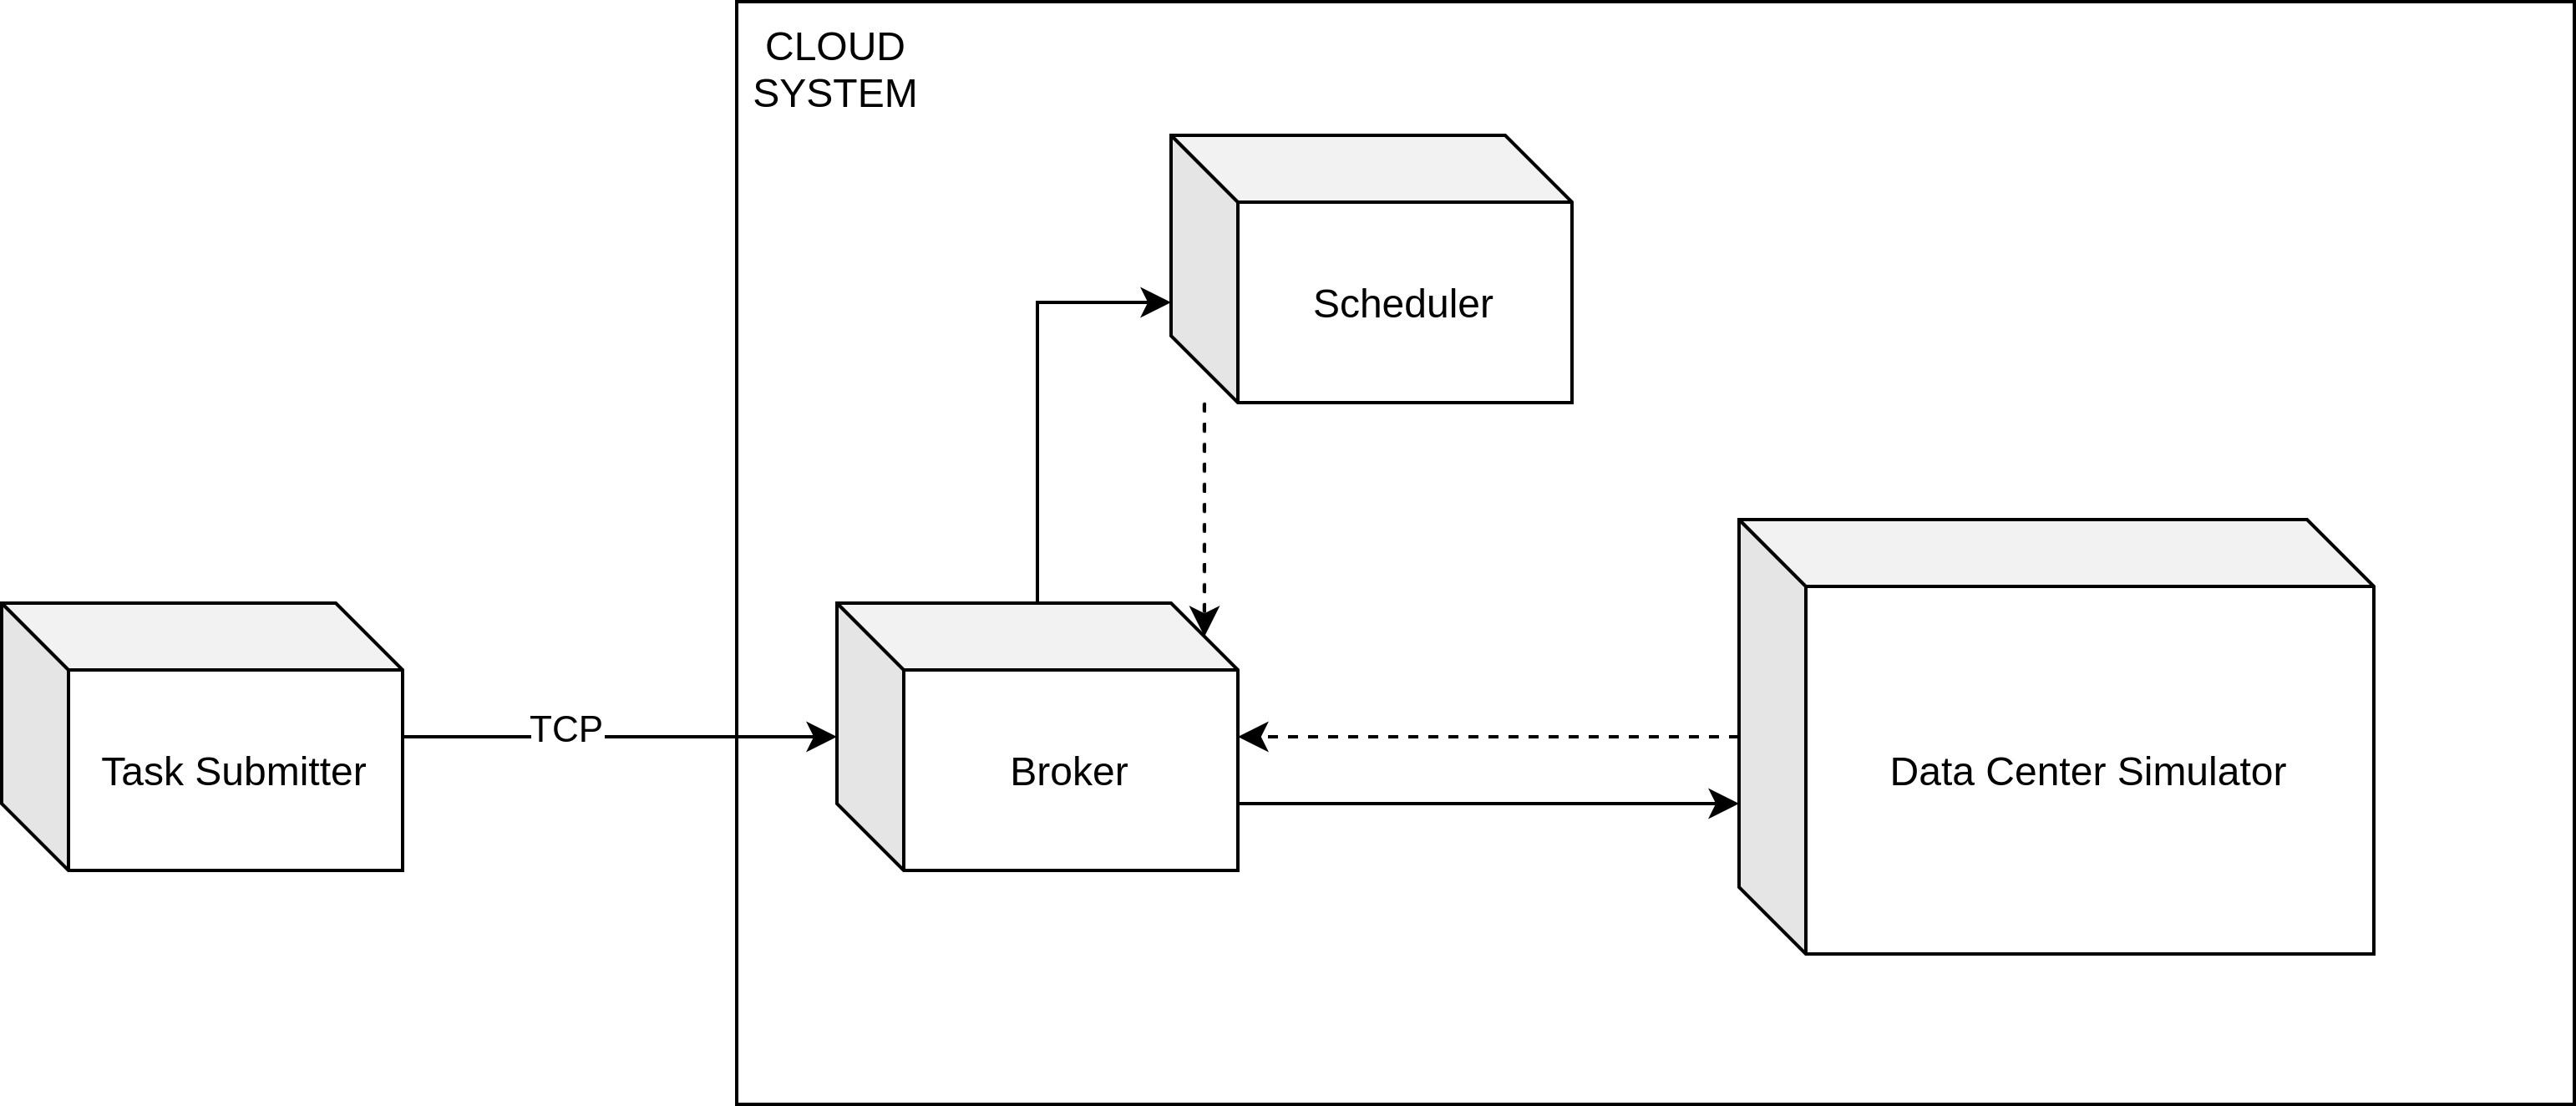
\includegraphics[scale=0.5]{images/simulation_system.png}
	\caption{Mô hình mô phỏng}
	\label{fig:simuation_system}
\end{figure}

\noindent
Các thành phần mô phỏng (hình ~\ref{fig:simuation_system}) bao gồm: 
\begin{itemize}
	\item \textbf{Task Submitter}: thành phần mô phỏng quá trình gửi tasks từ người dùng tới hệ thống cloud. Các tasks sẽ được gửi đi dưới dạng dữ liệu streaming. 
	\item \textbf{Broker}: thành phần mang chức năng làm trung gian giữa người dùng với hệ thống máy chủ, tiếp nhận tasks từ người dùng và chuyển chúng tới các máy tính ảo. Trong đồ án này, để phù hợp với xu hướng bùng nổ dữ liệu, Broker sử dụng nền tảng công nghệ Kafka để nhận các tasks được gửi tới, sau này có thể thực hiện thực nghiệm lập lịch phân tán. Để lựa chọn máy tính phù hợp cho tasks, Broker sử dụng bộ Scheduler thực hiện thuật toán lập lịch. 
	\item \textbf{Scheduler}: bộ lập lịch có nhiệm vụ ghép cặp giữa các tasks vào máy ảo.
	\item \textbf{Data Center Simulator}: bộ mô phỏng quá trình hoạt động của một hệ thống máy chủ. Được xây dựng trên nền tảng Cloudsim, Data Center Simulator có khả năng mô phỏng thời gian các tasks được thực thi trên các máy tính ảo, đưa ra thời gian thực thi của các tasks cùng với trạng thái tài nguyên của hệ thông trong quá trình mô phỏng.
\end{itemize}
Các thành phần trên đều được lập trình bằng ngôn ngữ java 14.\\
Thông số trong quá trình thực nghiệm: 
\begin{itemize}
	\item các tasks được gửi tới hệ thống theo phân phối $Poisson$ với trung bình 15 task/second
	\item thời gian đợi ở hàng chờ tối đa là 20 giây
	\item chỉ số K trong thuật toán~\ref{fig:algo3} bằng 3
	\item thời gian các tasks được chuyển từ bộ lập lịch đến máy ảo tuân theo phân phối chuẩn với kỳ vọng bằng 5 và độ lệch chuẩn bằng 0.5.
\end{itemize} 
% 6-8 pages
\section{Dữ liệu mô phỏng}
Dưới đây là thông số của 10 máy tính ảo được mô phỏng trong quá trình thực nghiệm. \\
\begin{table}[h!]
\centering
\caption{Bảng mô tả thông tin máy tính ảo}
\begin{tabular}{| p{1cm} | p{1cm} | p{1cm} | p{1.2cm} | p{1.2cm} | p{2cm} |}
	\hline
	\multicolumn{6}{|c|}{Virtual Machine Information List} \\
	\hline
	id & core	& mips & ram & storage & bandwidth \\
	   &       &      & (Mb)  & (Mb)   & (Mb/s) \\
	\hline
	\hline
	0&4 & 2000 & 4096 & 32768 & 16 \\
	\hline
	1&4&1000&8012&32768&16 \\
	\hline
	2&4&1000&4096&32768&16\\
	\hline
	3&4&2000&4096&32768&16\\
	\hline
	4&4&2000&8012&32768&16\\
	\hline
	5&4&1000&12288&32768&16\\
	\hline
	6&4&4000&12288&32768&16\\
	\hline
	7&4&1000&12288&32768&16\\
	\hline
	8&4&1000&4096&32768&16\\
	\hline
	9&4&2000&8012&32768&16\\
	\hline
\end{tabular}
\label{table:vm_info}
\end{table}

\noindent
Các dữ liệu về tasks trong quá trình mô phỏng được trích rút ngẫu nhiên từ 300G dữ liệu\cite{18} ghi lại từ hệ thống máy chủ của Google năm 2011.  Do bộ dữ liệu của Google không ghi lại các thông số về bandwidth và số lượng core mà task yêu cầu nên ta để mặc định lần lượt là 0 (Mb/s) và 2 (cores).
\begin{table}[!h]
    \begin{minipage}{.5\linewidth}
      \centering
        \caption{Tỉ lệ các kiểu công việc}
        \begin{tabular}{| p{3cm} | p{1cm} |}
            \hline
            \multicolumn{2}{|c|}{Type percentage} \\
            \hline
            type & \% \\
            \hline
            \hline
            long-running & 2\% \\
            \hline
            batch-job & 98\% \\
            \hline
        \end{tabular}   
	\label{table:types}          
    \end{minipage}%
    \begin{minipage}{.5\linewidth}
      \centering
        \caption{Phân phối mức độ ưu tiên của tasks}
        \begin{tabular}{| p{2cm} | p{0.5cm} |}
            \hline
            \multicolumn{2}{|c|}{Priorities percentage} \\
            \hline
            priority & \% \\
            \hline
            \hline
            0 & 90\% \\
            \hline
            1 & 10\% \\
            \hline
        \end{tabular}
	\label{table:priority}
    \end{minipage} 
\end{table}

\begin{table}[h!]
	\centering
	\caption{Tài nguyên yêu cầu}
        \begin{tabular}{| p{1.5cm} | p{1.5cm} | p{1.5cm} | p{1.5cm} |}
            \hline
            \multicolumn{4}{|c|}{Tasks' description} \\
            \hline
            stats & cpu & memory & storage \\
            	 & request (\%) & request (Mb) & request (Mb) \\
            \hline 
            \hline
            count & 30000 & 30000 & 30000 \\
            \hline
            mean & 0.051 & 24.93 & 11.0 \\
            \hline
            std & 0.056 & 40.35 & 5.2 \\
            \hline
            min & 0.006 & 1.24 & 0.1 \\
            \hline 
            25\% & 0.025 & 20.39 & 12.6 \\
            \hline 
            50\% & 0.025 & 26.75 & 12.6 \\
            \hline
            75\% & 0.313 & 26.75 & 12.6 \\
            \hline 
            max & 0.251 & 101.91 & 63.2 \\
            \hline
        \end{tabular}
	\label{table:request}
\end{table}

\noindent
Bảng~\ref{table:request} mô tả tài nguyên mà các tasks yêu cầu, bảng~\ref{table:types} mô tả phân phối giữa các kiểu của tasks, bảng~\ref{table:priority} mô tả phân phối về mức độ ưu tiên trong tập dữ liệu. 

\section{Thu thập dữ liệu xây dựng mạng Bayesian}
Phân phối xác suất của các đỉnh trong mạng Bayesian sẽ được học từ dữ liệu lịch sử của hệ thống. Ta chia bộ dữ liệu mô phỏng thành 2 phần ngẫu nhiễn với tỉ lệ 1:1, gọi là train và test. Công việc thu thập dữ liệu sẽ được thực hiện bằng việc mô phỏng hệ thống với thuật toán Worstfit trên tập train, cụ thể như sau: 
\begin{enumerate}
	\item Task được gửi tới hệ thống theo phân phối possion với trung bình 15 tasks/giây
	\item Trong quá trình hoạt động, ghi lại thông tin về các tasks đang chạy trong hệ thống tại thời điểm bắt đầu lập lịch ($t_{1}$) và thời điểm gửi các tasks mới tới các máy ảo ($t_{2}$). 
\end{enumerate}
Tại $t_{1}$, ta quan sát một job $J$ có các tasks $\{j_{1}, ..., j_{k}\}$ đều kiểu batch-job còn đang chạy. Ta cần tính: 
\begin{itemize}
	\item Xác suất job $J$ còn chạy tại thời điểm $t_{2}$
	\item Xác suất task $j_{i}$ còn chạy nếu biết $J$ còn chạy tại $t_{2}$
\end{itemize}
Sau khi tính được các tham số cho mạng Bayesian, ta sử dụng nó để chạy thuật toán lập lịch trong quá trình mô phỏng với bộ dữ liệu test. \\
Trong trường hợp môi trường thực tế, các dữ liệu sẽ được thu thập từ lịch sử hoạt động của hệ thống. Tham số của mạng Bayesian nên được cập nhật sau một khoảng thời gian nhất định để đáp ứng được với sự thay đổi về trạng thái của các tasks trong hệ thống. 
\section{Các tiêu chí đánh giá}
Mô hình lập lịch được đề xuất sử dụng mạng Bayesian để ước lượng trạng thái của các tasks trong quá trình lập lịch, từ đó đưa ra quyết định mà thích ứng được với các thay đổi trong quá trình chạy của hệ thống máy chủ. Để đánh giá được hiệu quả của mô hình, ta xem xét các tiêu chí sau: 
\begin{enumerate}
	\item \textit{Số lượng task hoàn thành trong một đơn vị thời gian}: Chỉ số này được dùng nhiều trong các nghiên cứu về thuật toán lập lịch. Với càng nhiều tasks được hoàn thành trong một khoảng thời gian, các chỉ số về thời gian hoàn thành công việc, thời gian chờ từ người dùng cũng sẽ được tối ưu. Bên cạnh đó, một hệ thống chấp nhận được thì số lượng task hoàn thành trong một đơn vị thời gian phải lớn hơn hoặc ngang bằng tỉ lệ task đến hệ thống, do đó, nếu là nhỏ hơn đáng kể thì ta phải xem xét lại độ chính xác của thuật toán hoặc suy nghĩ về việc mở rộng hệ thống. 
	\item \textit{Độ mất cân bằng khối lượng công việc giữa các máy}: Việc phân phối đều các tasks vào các máy ảo giúp tận dụng được tài nguyên của hệ thống và cân bằng tải trong hoạt hệ thống mạng. Hệ thống mất cân bằng khi phần trăm tài nguyên được sử dụng giữa các máy ảo chênh lệch quá lớn, và trong máy ảo bị sử dụng nhiều thì sẽ xảy ra hiện tượng đói tài nguyên. Việc tính chỉ số này đã được đưa ra trong thuật toán ~\ref{alg:2}. Như trong \ref{proposed_algo}, việc các tasks thay đổi trạng thái trong quá trình chạy sẽ phá vỡ sự cân bằng khối lượng công việc giữa các máy ảo, do đó, để đánh giá được sự ảnh hưởng của môi trường đến kết quả của thuật toán lập lịch, ta sẽ xem xét chỉ số này thay đổi theo thời gian hệ thống hoạt động. 
\end{enumerate} 

\section{Kết quả thực nghiệm}
\subsection{Số lượng task hoàn thành trong một đơn vị thời gian}
Kết quả mô phỏng 15000 tasks gửi đến hệ thống trong 1000s được mô mả trong bảng~\ref{table:finished_tasks}.
\begin{table}[h!]
	\centering
	\caption{Kết quả về thời gian chạy của các tasks}
	\begin{tabular}{|p{1.5cm}| p{1.5cm} | p{1.5cm} | p{1.6cm}|}
		\hline
		\multicolumn{4}{|c|}{Running statistics over 1000s} \\
		\hline
		stats & FCFS & Worstfit & Resources \\
			&	&	& balancing \\
		\hline
		\hline
		count&13214&13925&14235 \\
		\hline
		mean&10.62&6.34&5.42 \\
		\hline
		std&54.24&33.37&27.31 \\
		\hline
		min&0.31&0.12&0.21 \\
		\hline
		25\%&3.15&2.09&2.08 \\
		\hline
		50\%&5.78&3.52&3.41 \\
		\hline
		75\%&8.13&5.61&5.50 \\
		\hline
		max&829.92&616.35&640.39 \\
		\hline
	\end{tabular}
	\label{table:finished_tasks}
\end{table}
Trong 15000 tasks được gửi đến hệ thống, có 300 task là dạng long-running, vì vậy sẽ không kết thúc trong quá trình mô phỏng. Khi số lượng tasks đến lớn hơn số lượng tasks hoàn thành, các tasks chưa hoàn thành sẽ được tích lũy theo thời gian và chiếm tài nguyên của hệ thống. Đến khi tài nguyên không đủ, các tasks với mức ưu tiên thấp sẽ bị hủy và quay lại hàng chờ để nhường tài nguyên cho các tasks có mức ưu tiên cao. Trong bảng~\ref{table:finished_tasks}, ta thấy số lượng tasks hoàn thành của \textbf{thuật toán được đề xuất (Resources Balancing)} trong 1000s là cao nhất, 14235 tasks so với 13925 của Worstfit và 13214 của FCFS (First Come First Serve). Thời gian trung bình hoàn thành 1 tasks của Resources Balancing là 5.42 giây, bằng một nửa của FCFS, là giá trị nhỏ nhất trong 3 thuật toán. Trong sự so sánh giữa Resources balancing với Worstfit, ta thấy thống kê min, max thời gian thực thi của thuật toán đề xuất đều lớn hơn, nhưng về mặt trung bình thì lại nhỏ hơn. Điều này là bởi vì Resources balancing vừa cân bằng cho khối lượng batch-job, vừa cho long-running, nên quyết định lập lịch cho các phần tử riêng biệt như task ngắn nhất và dài nhất sẽ không tốt bằng Worstfit - thuật toán tìm máy ảo phù hợp nhất cho cá nhân từng tasks. Nhưng về tổng thể trong suốt quá trình hoạt động, thuật toán đề xuất tỏ ra hiệu quả hơn. 

\subsection{Ảnh hưởng của thời gian trễ tới sai số}
Ta đã biết 
\[
	\delta_{t} = t_{2} - t_{1} = time_{scheduling} + network\_delay
\]
là thời gian trễ của thông tin trong quá trình lập lịch, từ thời điểm lập lịch tới thời điểm thực thi. Trong đó: 
\begin{itemize}
	\item $time_{scheduling}$ là thời gian chạy thuật toán lập lịch, phụ thuộc vào độ phức tạp của thuật toán, số lượng máy ảo, số lượng tasks, khả năng tính toán của máy tính thực hiện việc lập lịch.
	\item $network\_delay$ là thời gian thông tin truyền tin trong mạng, bao gồm việc truyền thông tin trạng thái hệ thống tới bộ lập lịch và việc gửi các tasks đến máy ảo tương ứng để thực thi.
\end{itemize} 
Thông thường, các thuật toán heuristic sẽ có độ phức tạp không quá lớn, nên thời gian lập lịch sẽ không đóng góp nhiều vào tổng thời gian trễ. Tuy nhiên, trong môi trường dữ liệu lớn, tỉ lệ tasks đến hệ thống được tính bằng hàng triệu tasks một giây, thời gian lập lịch sẽ đóng góp tương đương hoặc hơn so với thời gian truyền tin trong mạng.
\begin{figure}[h!]
	\centering
	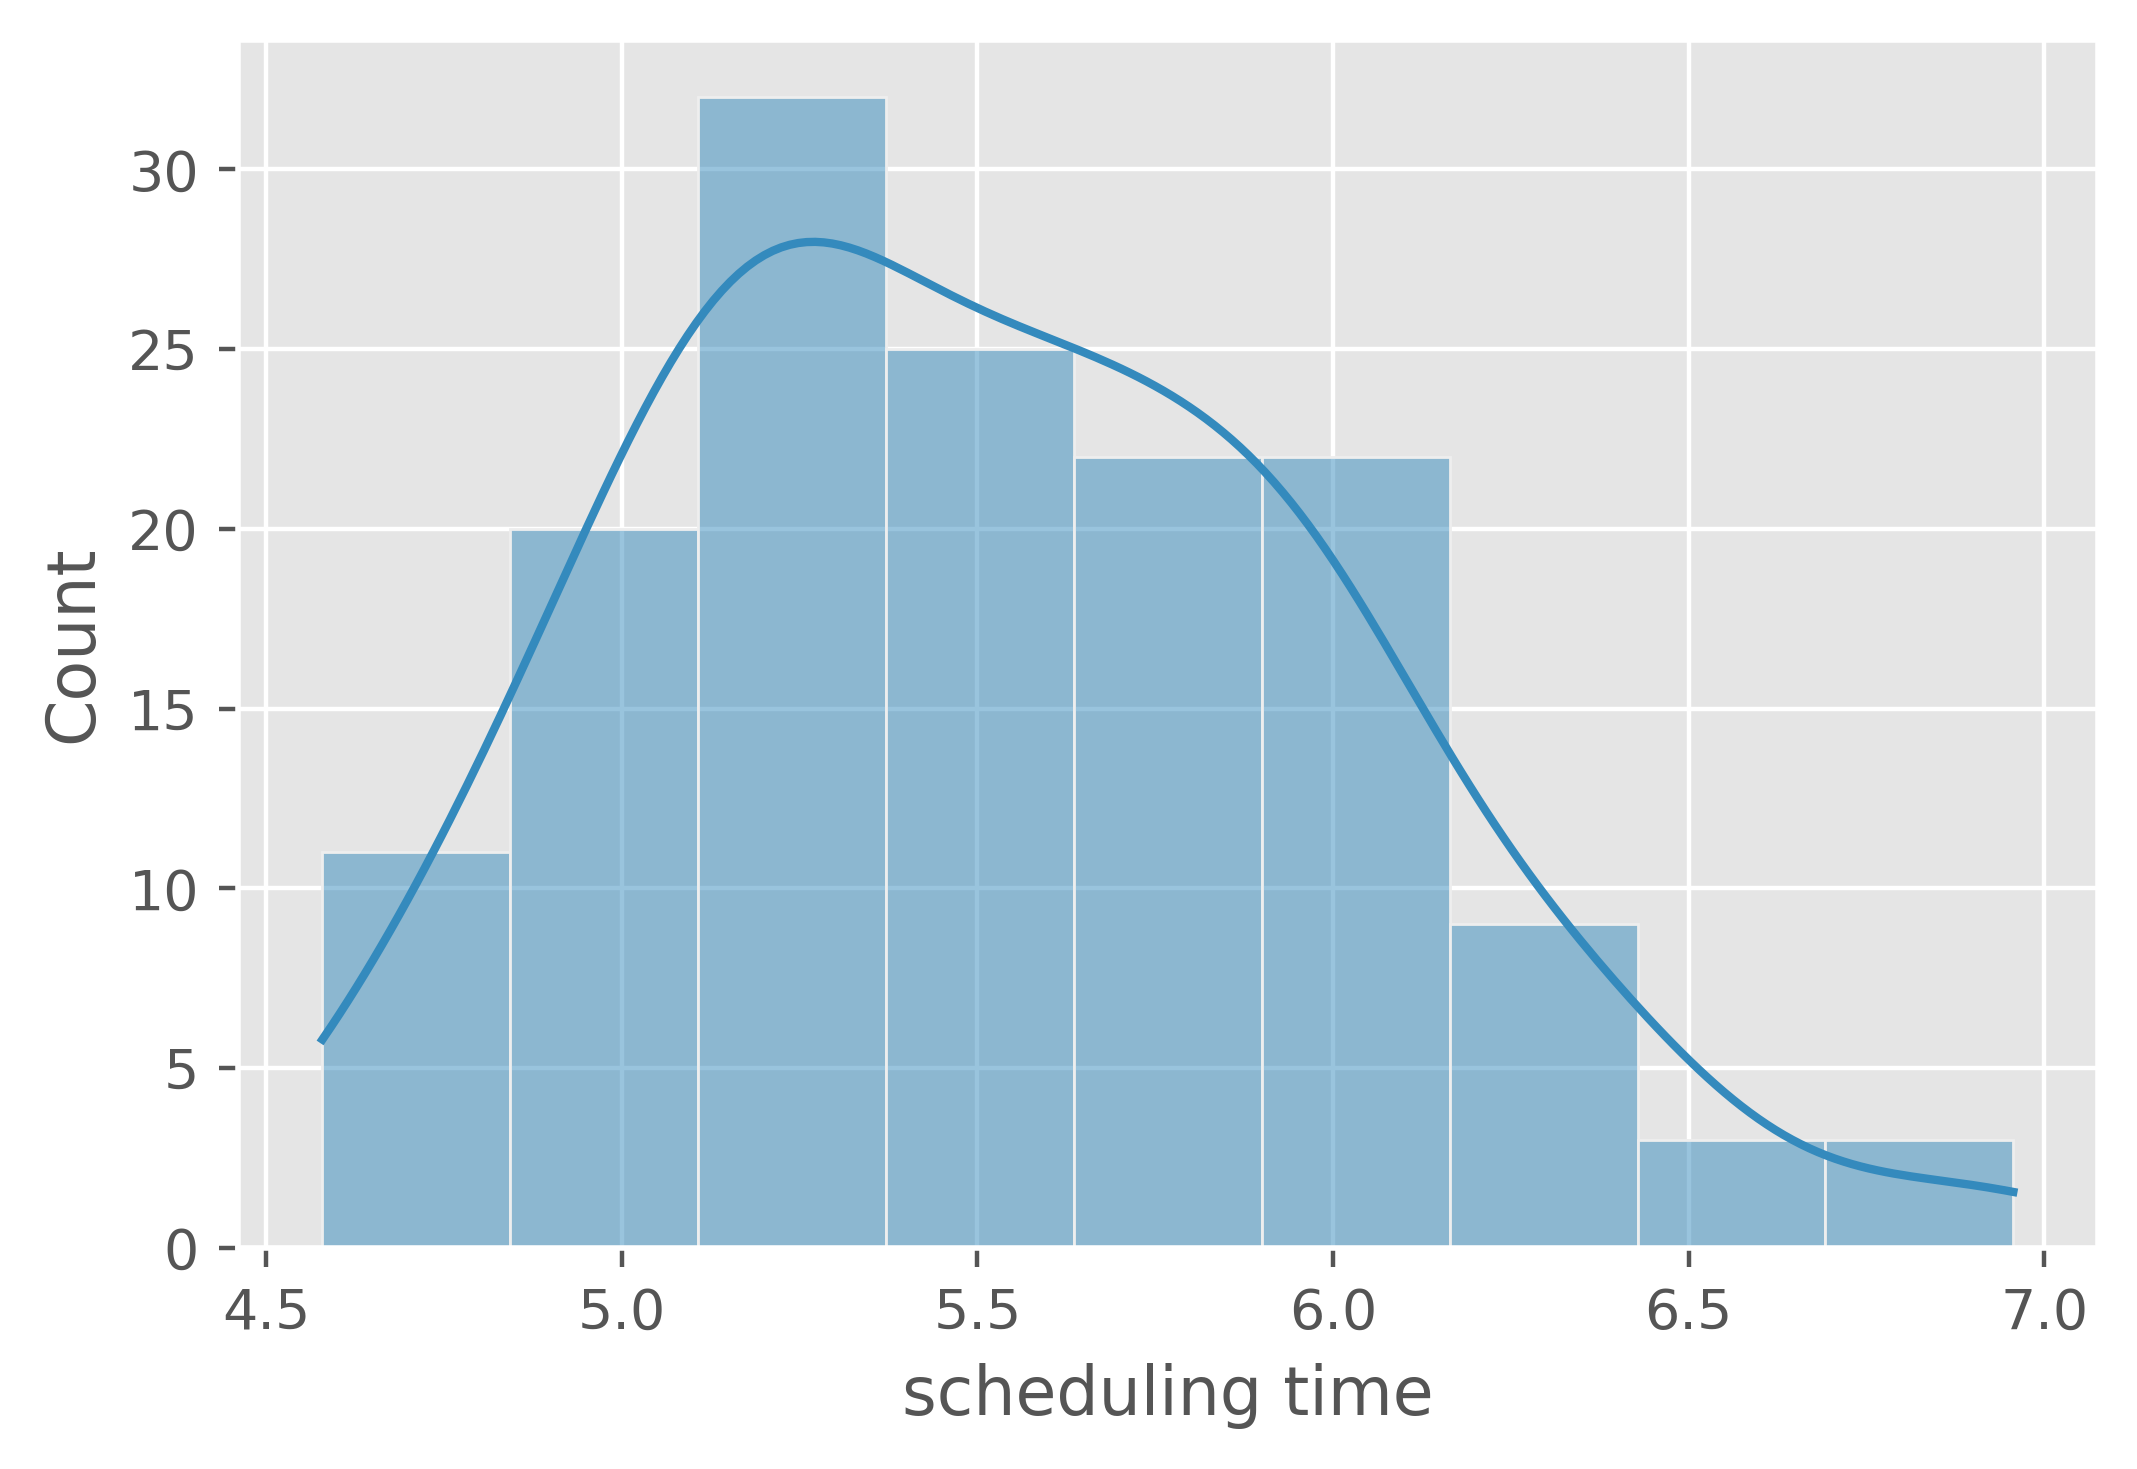
\includegraphics[scale=0.8]{images/scheduling_time_distribution.png}
	\caption{Phân phối của độ trễ trong quá trình mô phỏng}
	\label{fig:scheduling_time_dist}
\end{figure}

\noindent
Trong hình~\ref{fig:scheduling_time_dist}, khoảng thời gian trễ từ thời điểm lập lịch với thời điểm thực thi trong quá trình mô phỏng với thuật toán Worstfit được phân bố theo phân phối chuẩn với: 
\[
	E[\delta_{t}] = 5.5 , V[\delta_{t}] = 0.55^{2}
\]
Với thuật toán Worstfit, ta có hơn 50\% tasks có thời gian lập lịch nhỏ hơn 5 giây (trong bảng~\ref{table:finished_tasks}), như vậy tại thời điểm lập lịch nếu có N tasks đang chạy trong hệ thống thì sẽ có trung bình lớn hơn N / 2 tasks kết thúc trong quá trình lập lịch. \\
\begin{figure}[h!]
	\centering
	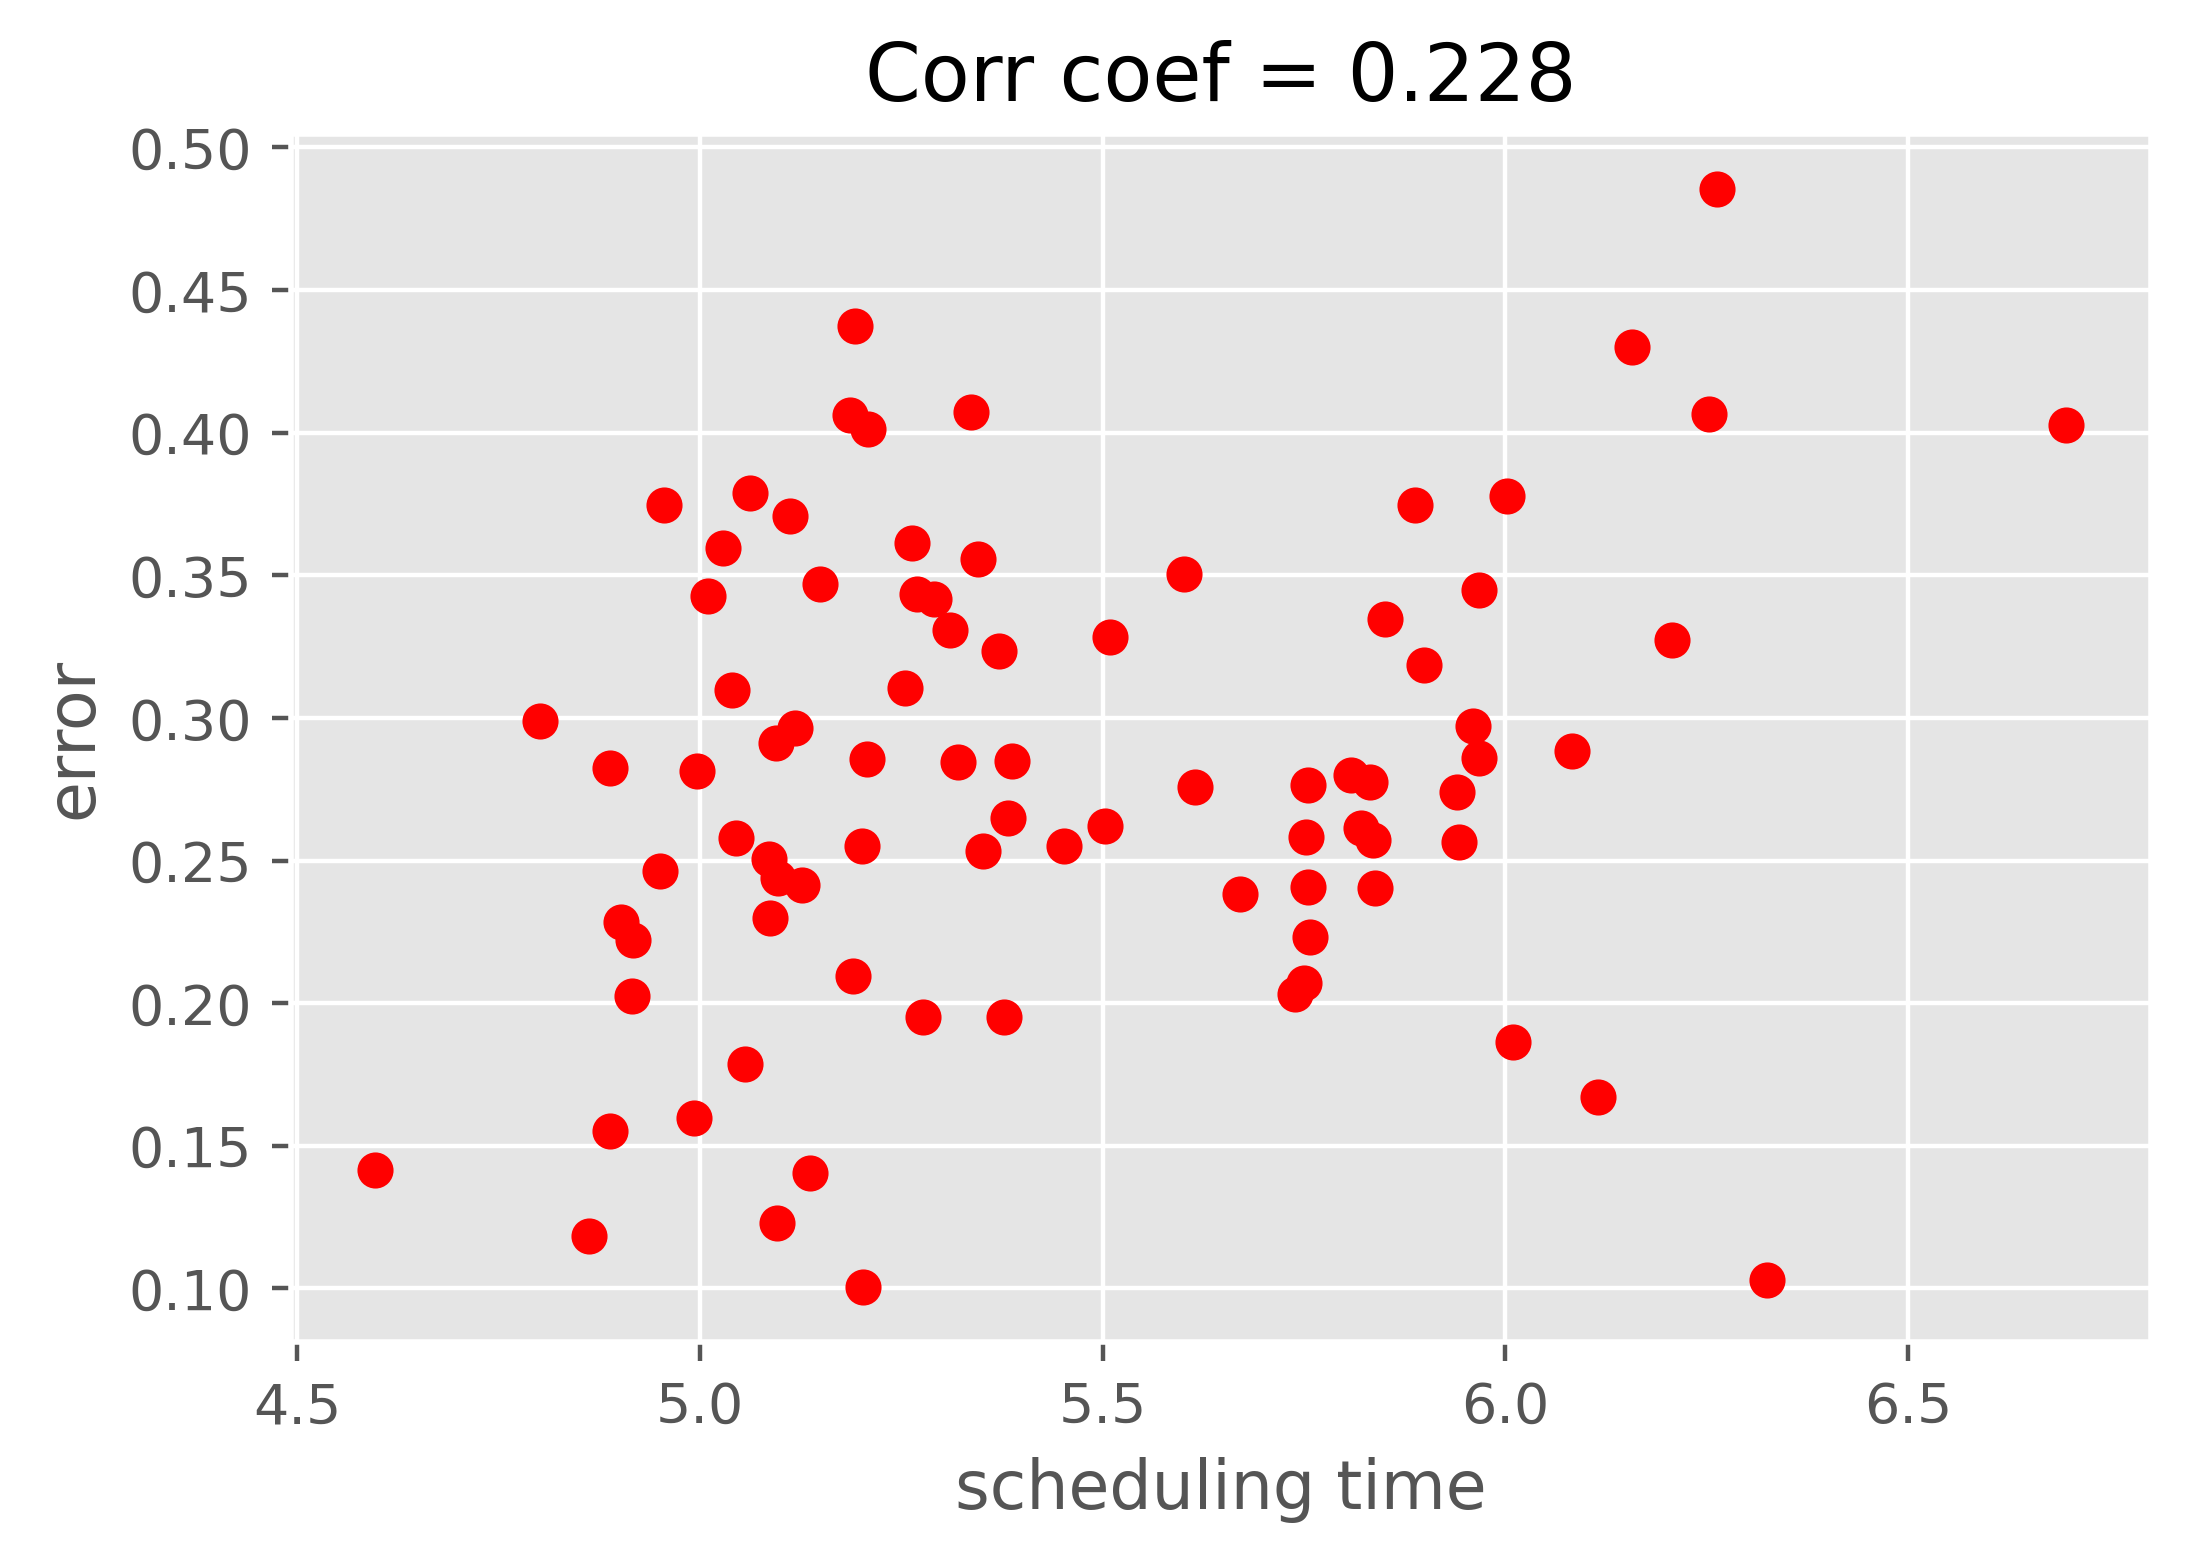
\includegraphics[scale=0.8]{images/scheduling_time_vs_delta.png}
	\caption{Thời gian trễ ảnh hưởng tới độ sai lệch}
	\label{fig:time_vs_error}
\end{figure}

\noindent
Trong hình~\ref{fig:time_vs_error} là thể hiện độ sai lệch của lượng tài nguyên CPU đã sử dụng tại thời điểm lập lịch với thời điểm thực thi. Với hệ số tương quan bằng 0.228, có thể thấy rằng với thời gian trễ càng lâu, sai lệch tại hai thời điểm trên sẽ càng tăng. \\

\subsection{Ảnh hưởng của thời gian trễ tới kết quả lập lịch}
\textit{Liệu rằng thời gian trễ trong quá trình lập lịch có khiến kết quả của việc lập lịch kém hiệu quả hơn không?} \\ 
Để trả lời cho câu hỏi trên, ta thực hiện thực nghiệm mô phỏng để kiếm chứng xem sự việc dùng thông tin bị trễ để lập lịch có khiến cho thời gian hoàn thành các tasks tăng lên hay không? \\
Ta sẽ chọn ngẫu nhiên một lượng tasks trong tập dữ liệu trích rút được từ bộ dữ liệu của Google, sau đó tiến hành mô phỏng chúng được lập lịch bằng thuật toán Worstfit với 2 kịch bản: 
\begin{itemize}
	\item Kịch bản 1: Ta giữ thông tin lập lịch không bị trễ bằng cách tạm dừng quá trình mô phỏng trong thời gian lập lịch, sau khi lập lịch xong thì mới tiếp tục mô phỏng. Như vậy, trạng thái của các tasks đang chạy trong hệ thống sẽ không bị thay đổi trong quá trình mô phỏng do chúng bị tạm dừng. 
	\item Kịch bản 2: Quá trình lập lịch sẽ chạy song song với quá trình mô phỏng, như vậy sẽ có sự sai khác giữa thông tin tại thời điểm lập lịch với thời điểm thực thi. 
\end{itemize}
Kết quả thu được trên bộ dữ liệu chọn ngẫu nhiên gồm 266 tasks được mô tả như hình \ref{fig:delay_impact}. 
\begin{figure}[h!]
	\centering
	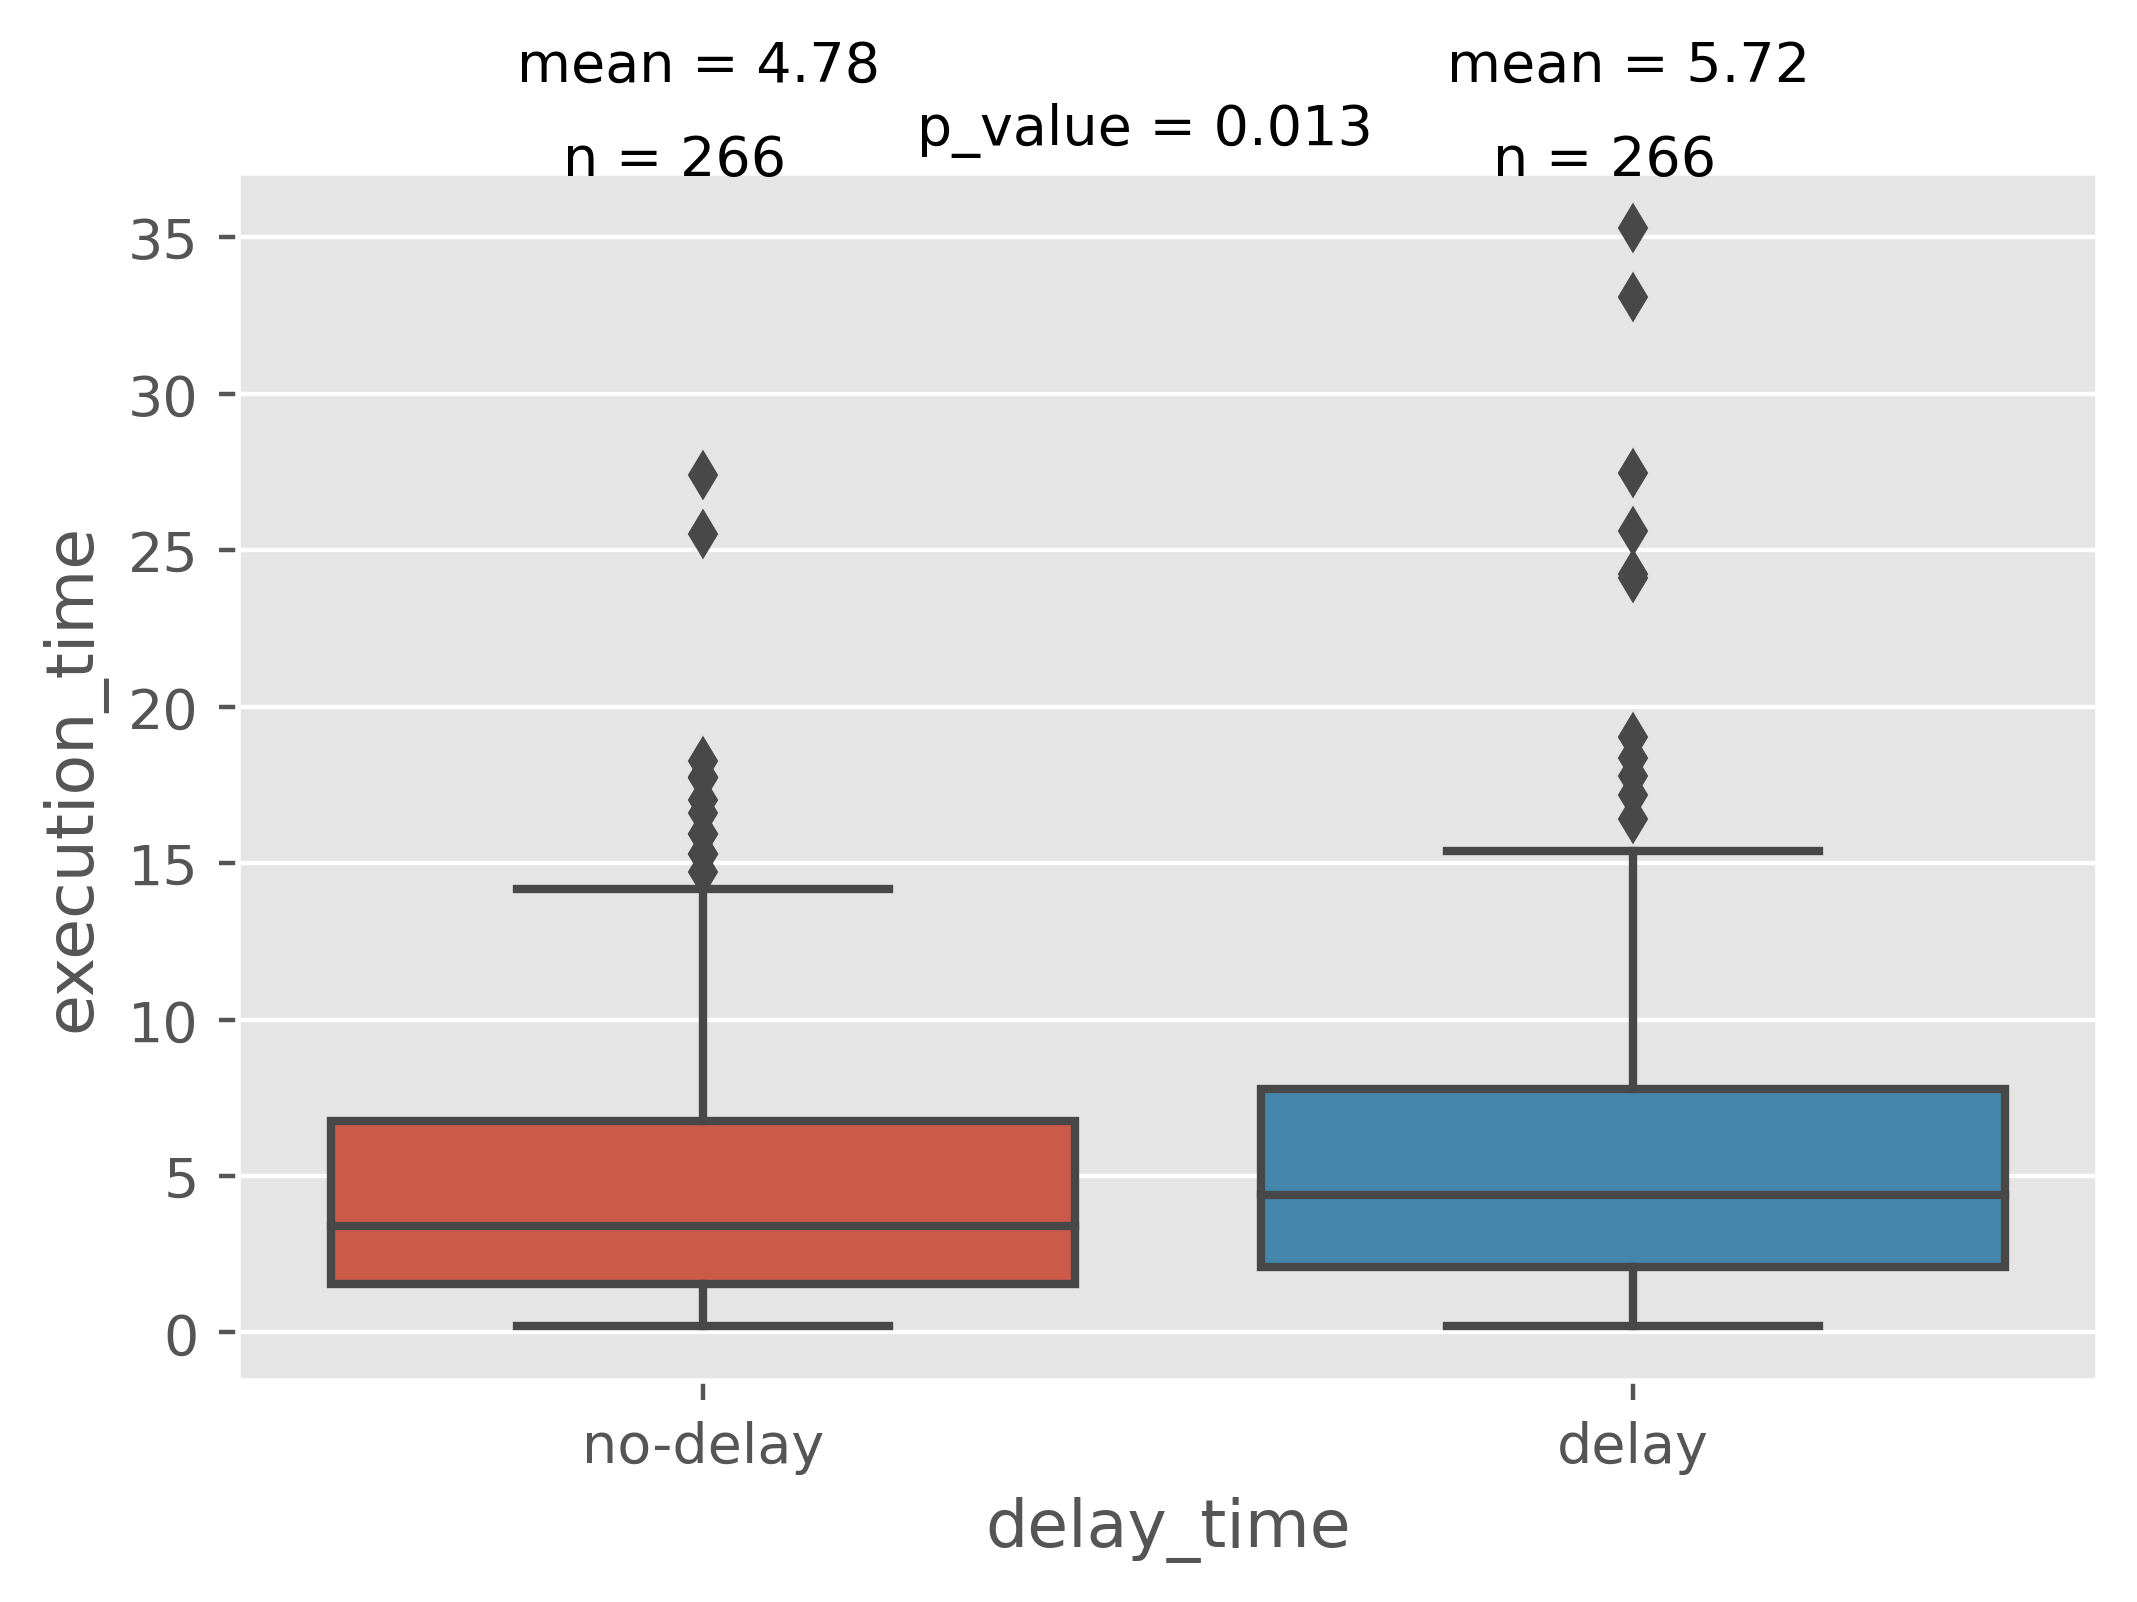
\includegraphics[scale=0.8]{images/delay_impact.png}
	\caption{Ảnh hưởng của sự trễ với thời gian thực thi}
	\label{fig:delay_impact}
\end{figure}

\noindent
Ta thấy rằng kịch bản thứ nhất (no-delay) có trung bình thời gian thực thi nhỏ hơn so với kịch bản thứ 2 (delay), ứng với số liệu là 4.78 và 5.72. Với giá trị $pvalue = 0.013$ và mức ý nghĩa $\alpha = 0.05$, ta có thể kết luận rằng việc lập lịch với các thông tin bị trễ khiến cho thời gian thực thi của tasks tăng lên. 

\subsection{Hiểu quả của việc ước lượng tài nguyên}
Ta sẽ so sánh sự khác biệt giữa việc sử dụng mạng Bayesian để ước lượng tài nguyên khả dụng với việc dùng thông tin tại thời điểm bắt đầu lập lịch. Xét tại thời điểm lập lịch $t_{1}$, với máy tính ảo vm, ta thu được tập các tasks đang chạy là $r = \{task_{1}, ..., task_{k}\}$. Tại thời điểm lập lịch hoàn thành và các tasks mới đến được đưa đến vm, $t_{2}$, các tasks trong tập $r$ có thể đã hoàn thành và tài nguyên được giải phóng. Gọi $q = \{s_{1}, ..., s_{k}\}$ là trạng thái của các tasks trong $r$ tại thời điểm $t_{2}$, 
\[
s_{i} = 
	\begin{cases}
		\text{0, } &\quad\text{nếu $task_{i}$ còn chạy tại thời điểm $t_{2}$} \\
		\text{1, } &\quad\text{nếu $task_{i}$ kết thúc trong quá trình lập lịch}
	\end{cases}
\]
Với các thuật toán thông thường, khi ta lấy thông tin tại $t_{1}$ để lập lịch, tài nguyên khả dụng của máy ảo được tính: 
\[
	hard\_est\_resources = vm.v - \sum_{i = 1}^{k}task_{i}.c
\]
Như tại thời điểm $t_{2}$, lượng tài nguyên thực tế khả dụng là: 
\[
	real\_resources = vm.v - \sum_{i = 1}^{k}task_{i}.c \times s_{i}
\]
Do 
\[
	\sum_{i = 1}^{k}task_{i}.c \times s_{i} \leq \sum_{i = 1}^{k}task_{i}.c
\]
nên 
\[
	real\_resources \geq hard\_est\_resources
\]
Khi sử dụng mạng Bayesian để tính $p_{i}$ là xác suất $task_{i}$ còn chạy tại $t_{2}$, tài nguyên ước lượng là: 
\[
	est\_resources = vm.v - \sum_{i = 1}^{k}task_{i}.c \times p_{i}
\]
Tương tự, ta có:
\[
	est\_resources \geq hard\_est\_resources
\]
Để thấy được rõ ràng sự chênh lệch giữa các phương pháp, ta ghi lại các kết quả ước lượng được với thông tin thực tế thu được xuyên suốt quá trình mô phỏng.
Trong hình~\ref{fig:usage_est_a}, đường màu tím biểu diễn cho $hard\_est\_resources$, là thông tin không được ước lượng. Do thời gian trung bình chạy của các tasks chỉ khoảng 5 giây (bảng~\ref{table:finished_tasks}), nên sự thay đổi trạng thái liên túc của các tasks khiến cho việc ước lượng với thực tế bị chênh lệch rất nhiều. Kết quả ước lượng bằng mạng Bayesian được thể hiện bằng đường màu đỏ, dao động xung quanh đường giá trị thực và có sai số nhỏ hơn so với việc dùng thông tin bị trễ. 

\begin{figure}[t]
\centering
\begin{subfigure}{.5\textwidth}
  \centering
  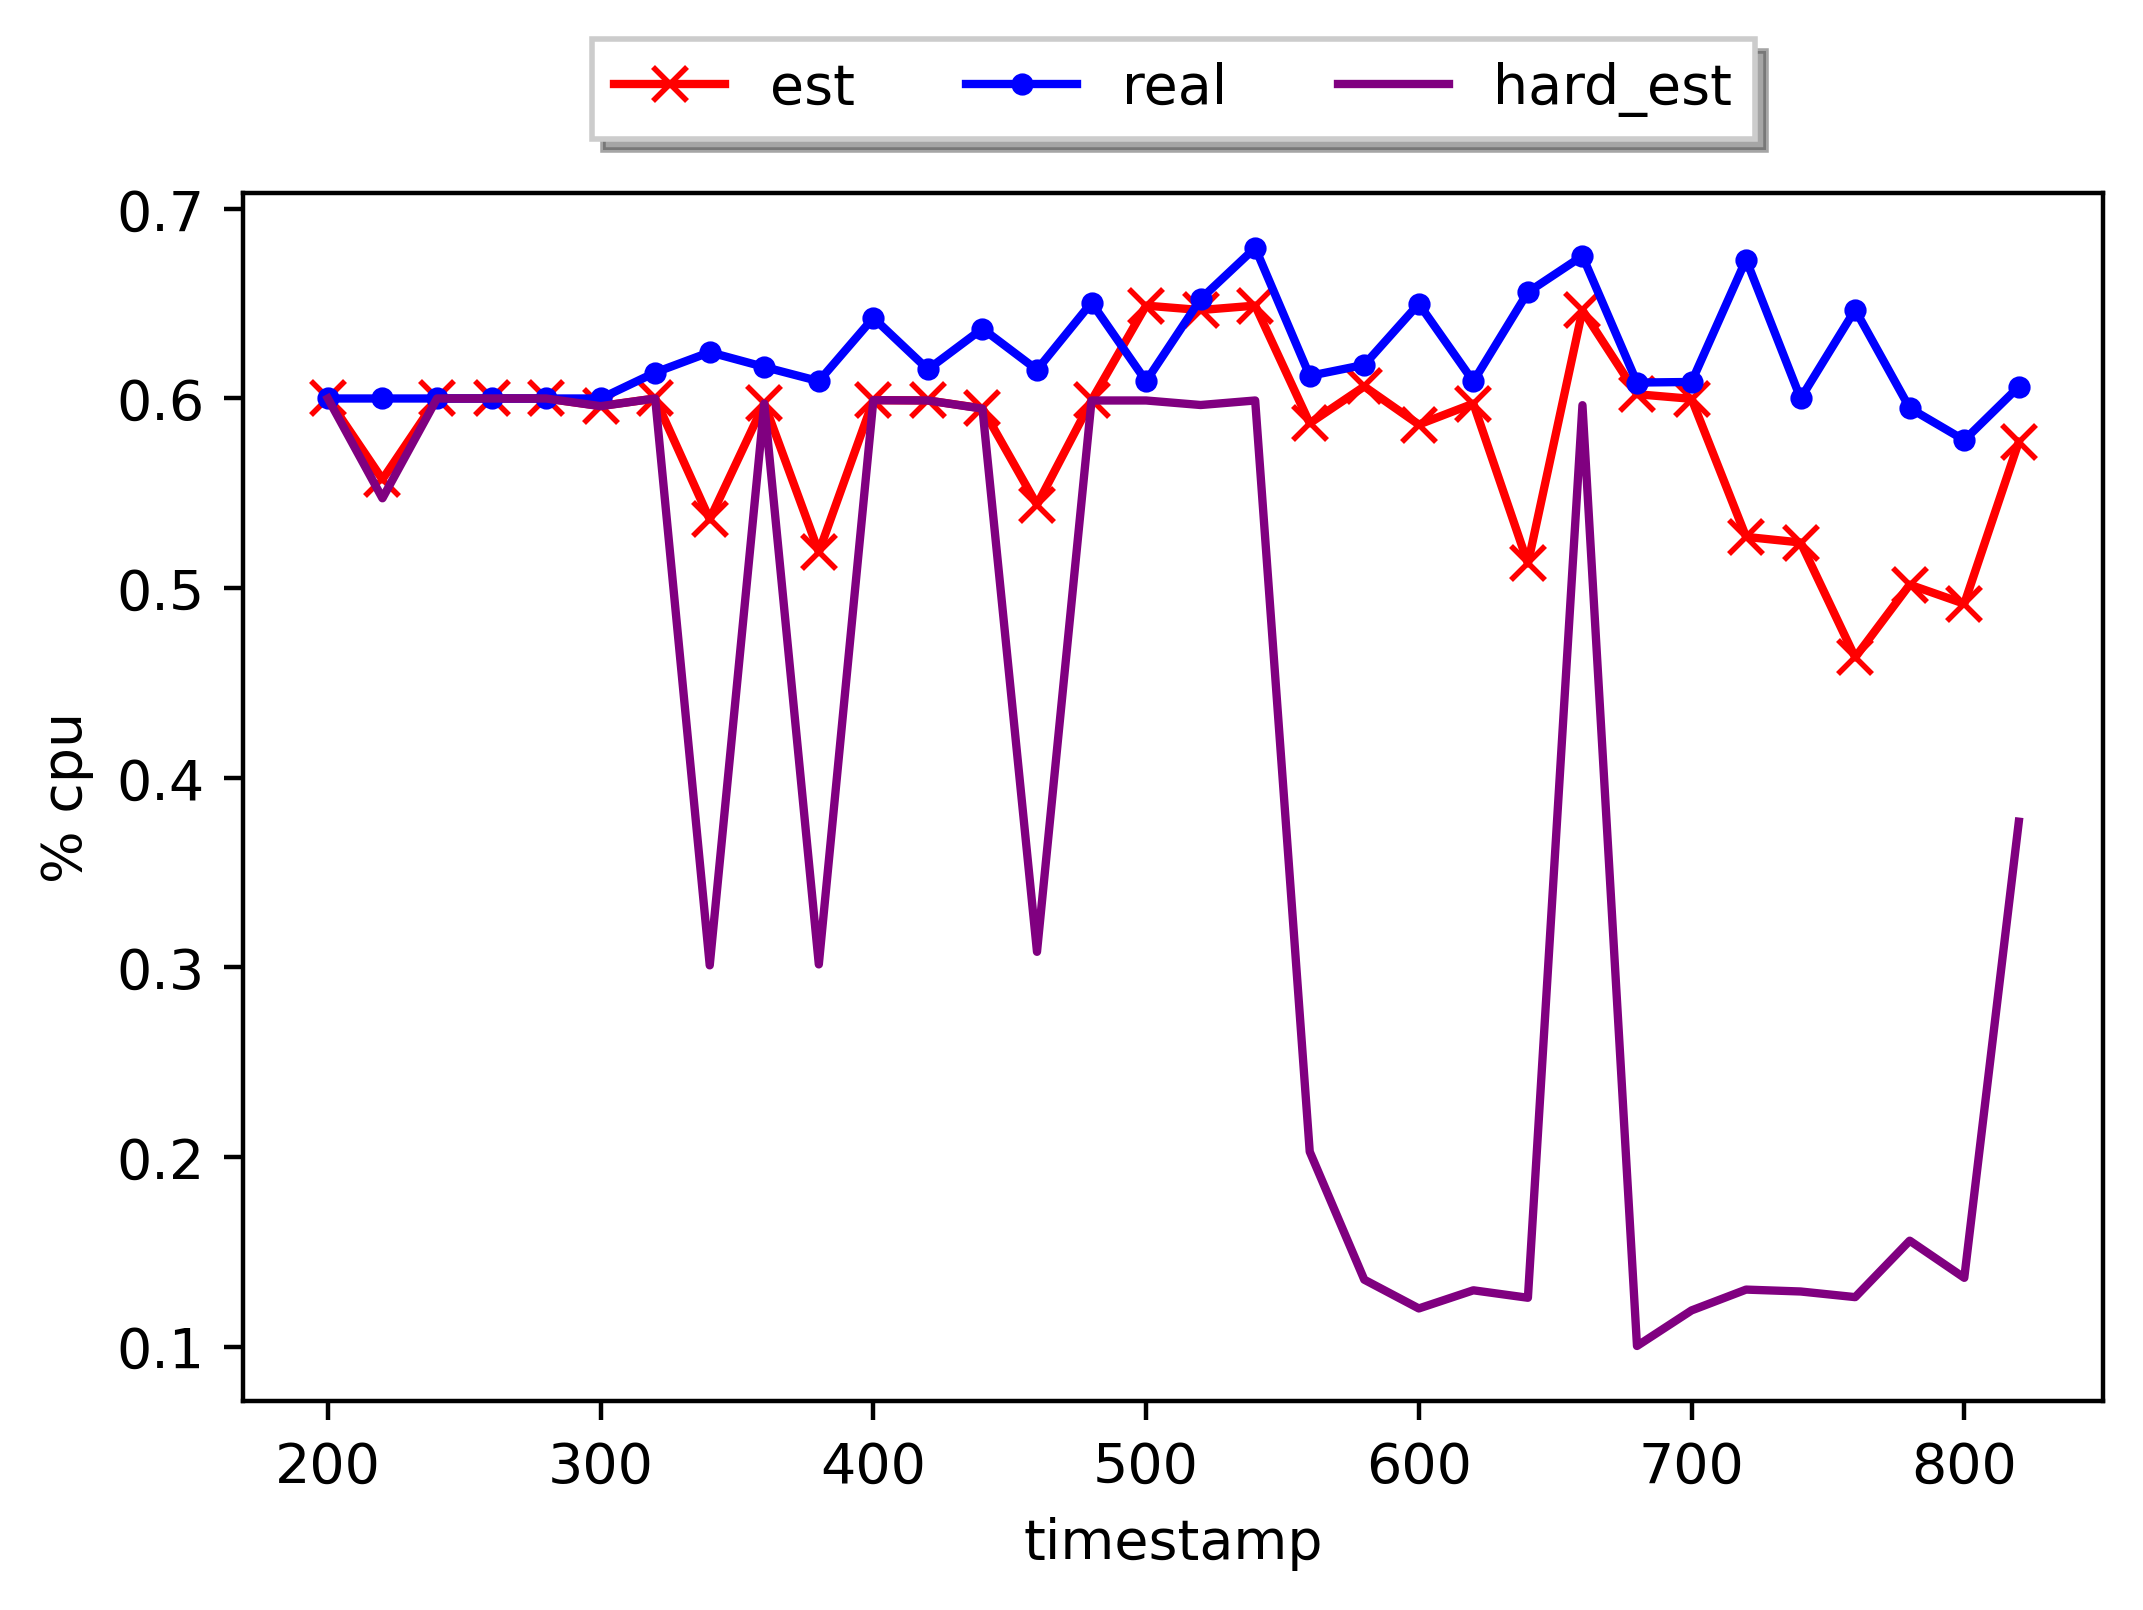
\includegraphics[width=.85\linewidth]{images/cpu_usage_estimation_1.png}
  \caption{Tài nguyên khả dụng tại thời điểm thực thi}
  \label{fig:usage_est_a}
\end{subfigure}%
\begin{subfigure}{.5\textwidth}
  \centering
  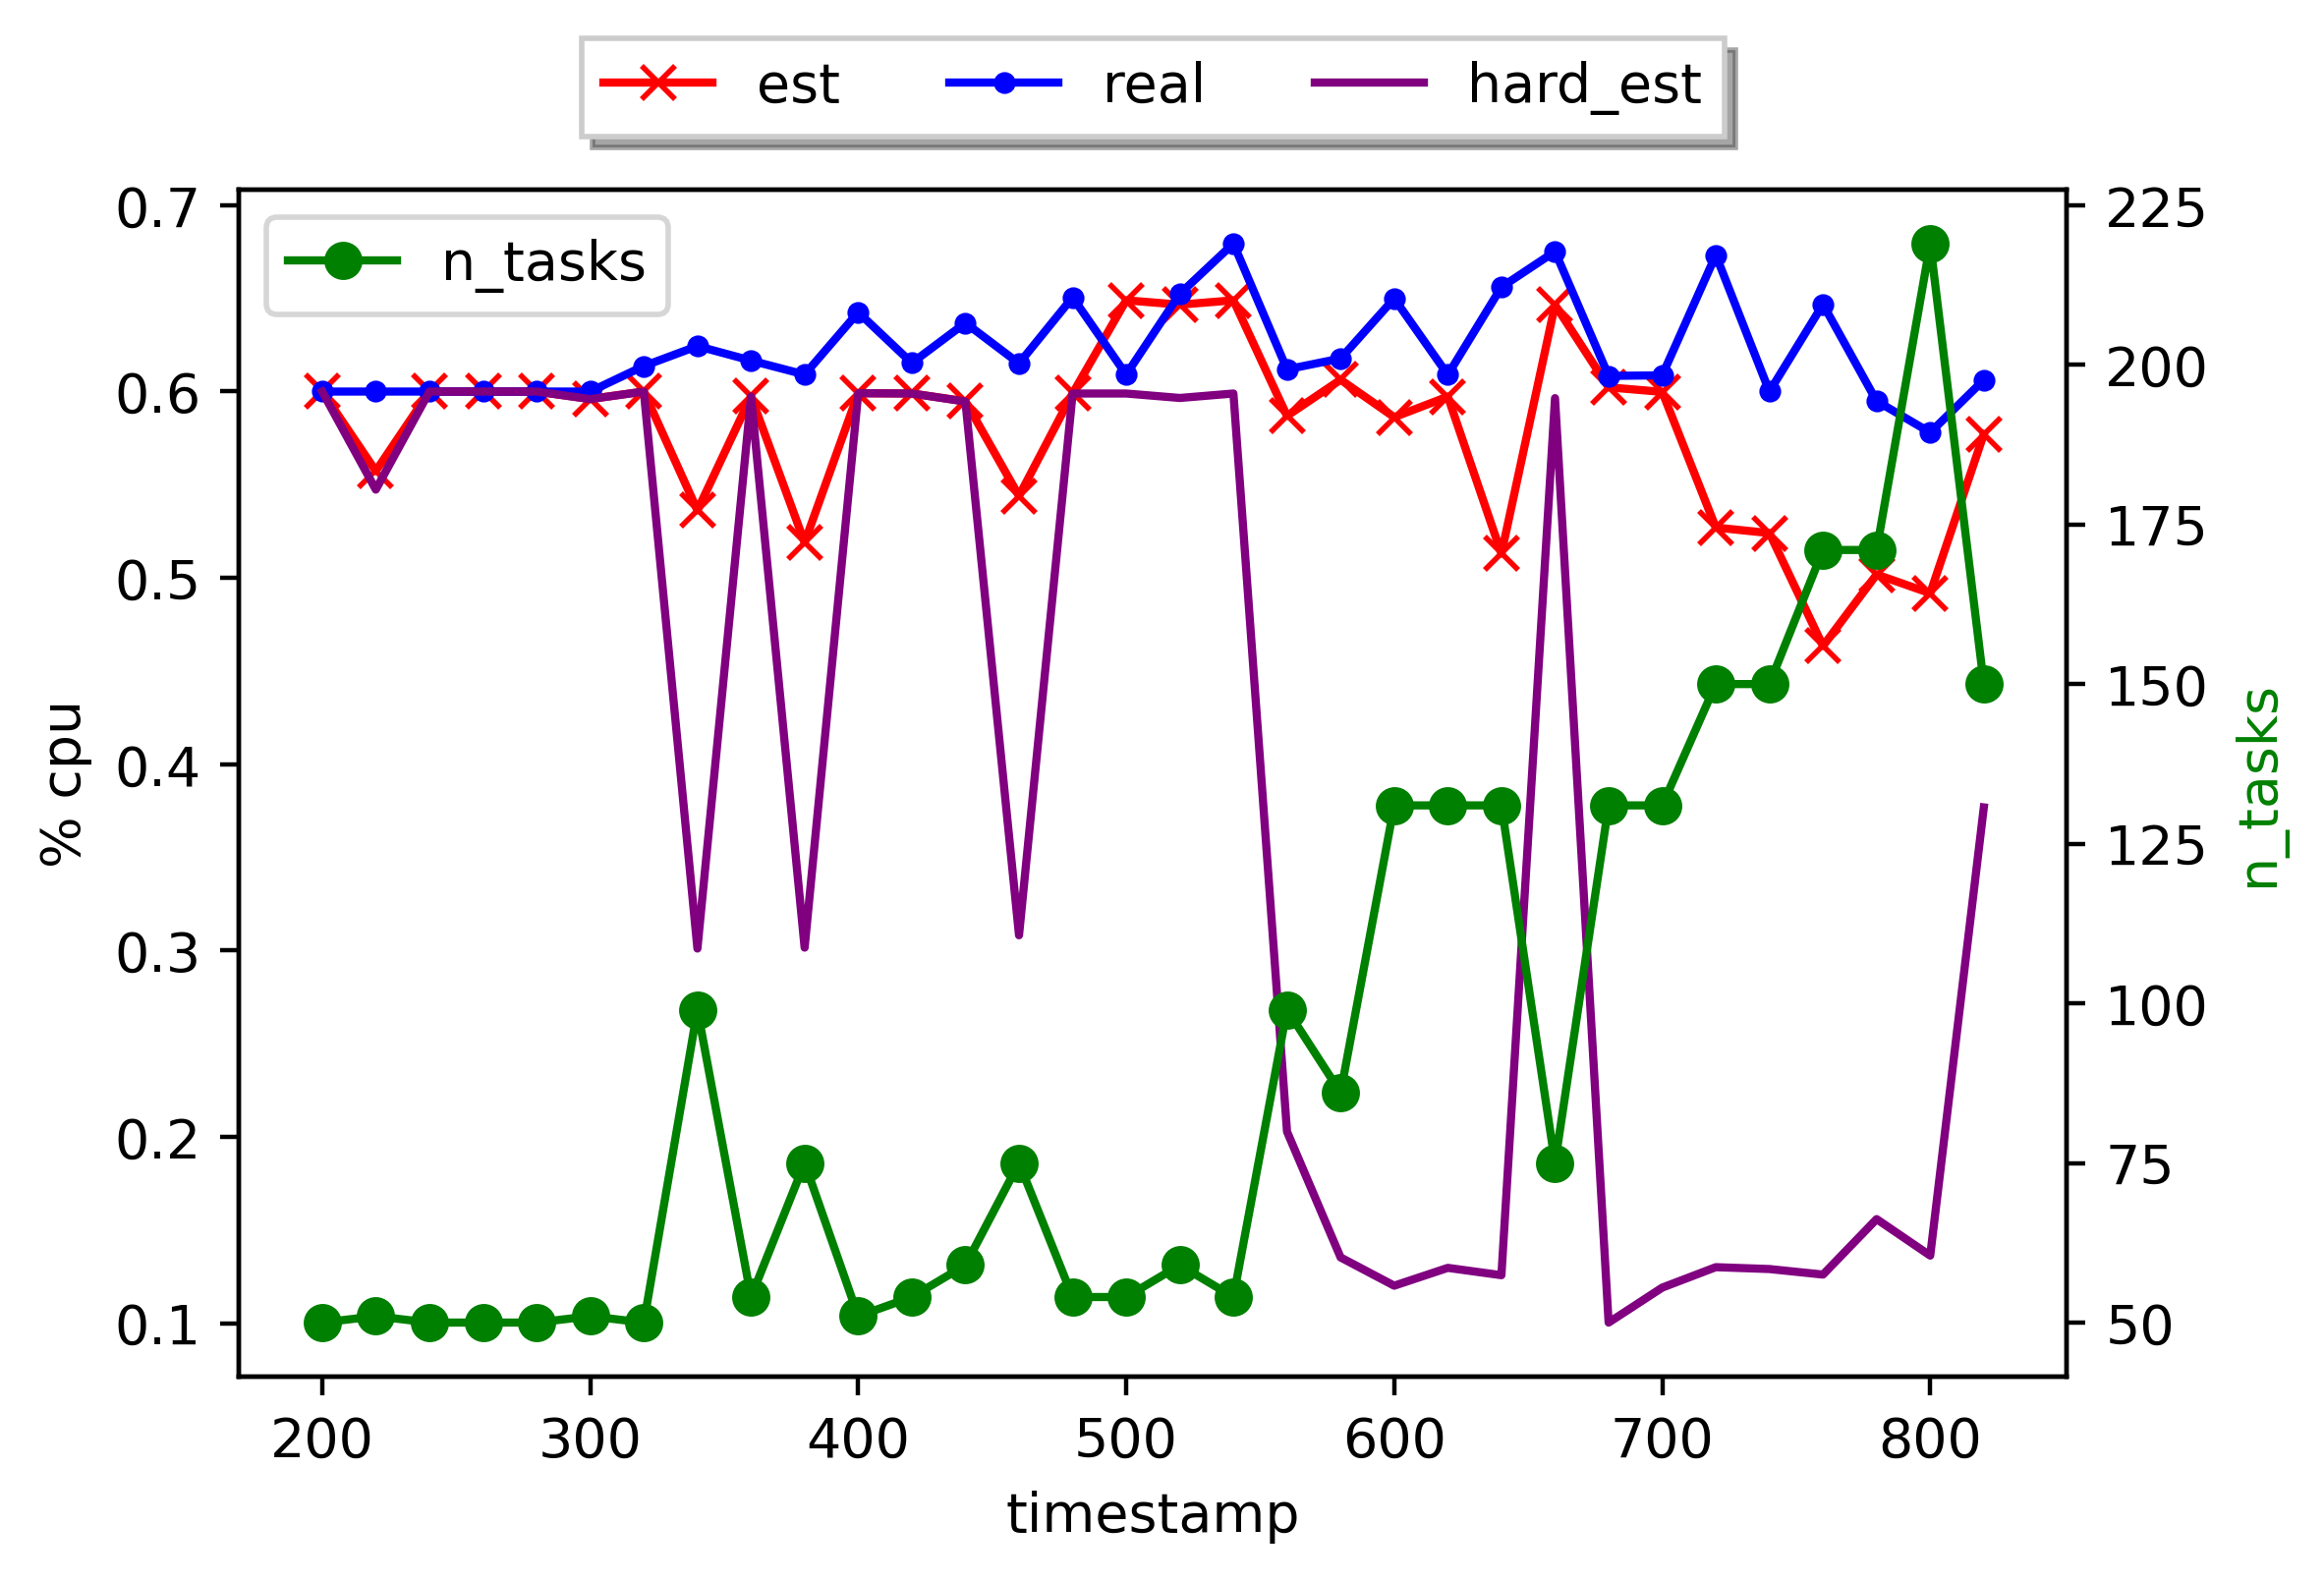
\includegraphics[width=.9\linewidth]{images/cpu_usage_estimation_2.png}
  \caption{Ảnh hưởng của số lượng tasks đang chạy}
  \label{fig:usage_est_b}
\end{subfigure}
\caption{Thông số tại thời điểm kết thúc lập lịch}
\label{fig:usage_est}
\end{figure}

\noindent
Mức độ sai lệch của cả hai phương pháp đều phụ thuộc vào số lượng tasks đang chạy trong máy ảo. Hình~\ref{fig:usage_est_b} cho thấy khi số lượng tasks càng tăng (đường màu xanh lá cây), sai số do độ chễ của hệ thống cùng với sai số của mạng Bayesian đều tăng lên. Dù vậy, về tổng quan, việc ước lượng cũng có sai số nhỏ hơn với việc dùng thông tin bị trễ, và hiệu quả của nó giúp cải thiện sự mất cân bằng của hệ thống do sự thay đổi trạng thái của các tasks trong hệ thống. 

\subsection{Sự mất cân bằng khối lượng công việc giữa các máy trong quá trình hoạt động}
\begin{figure}[h!]
	\centering
	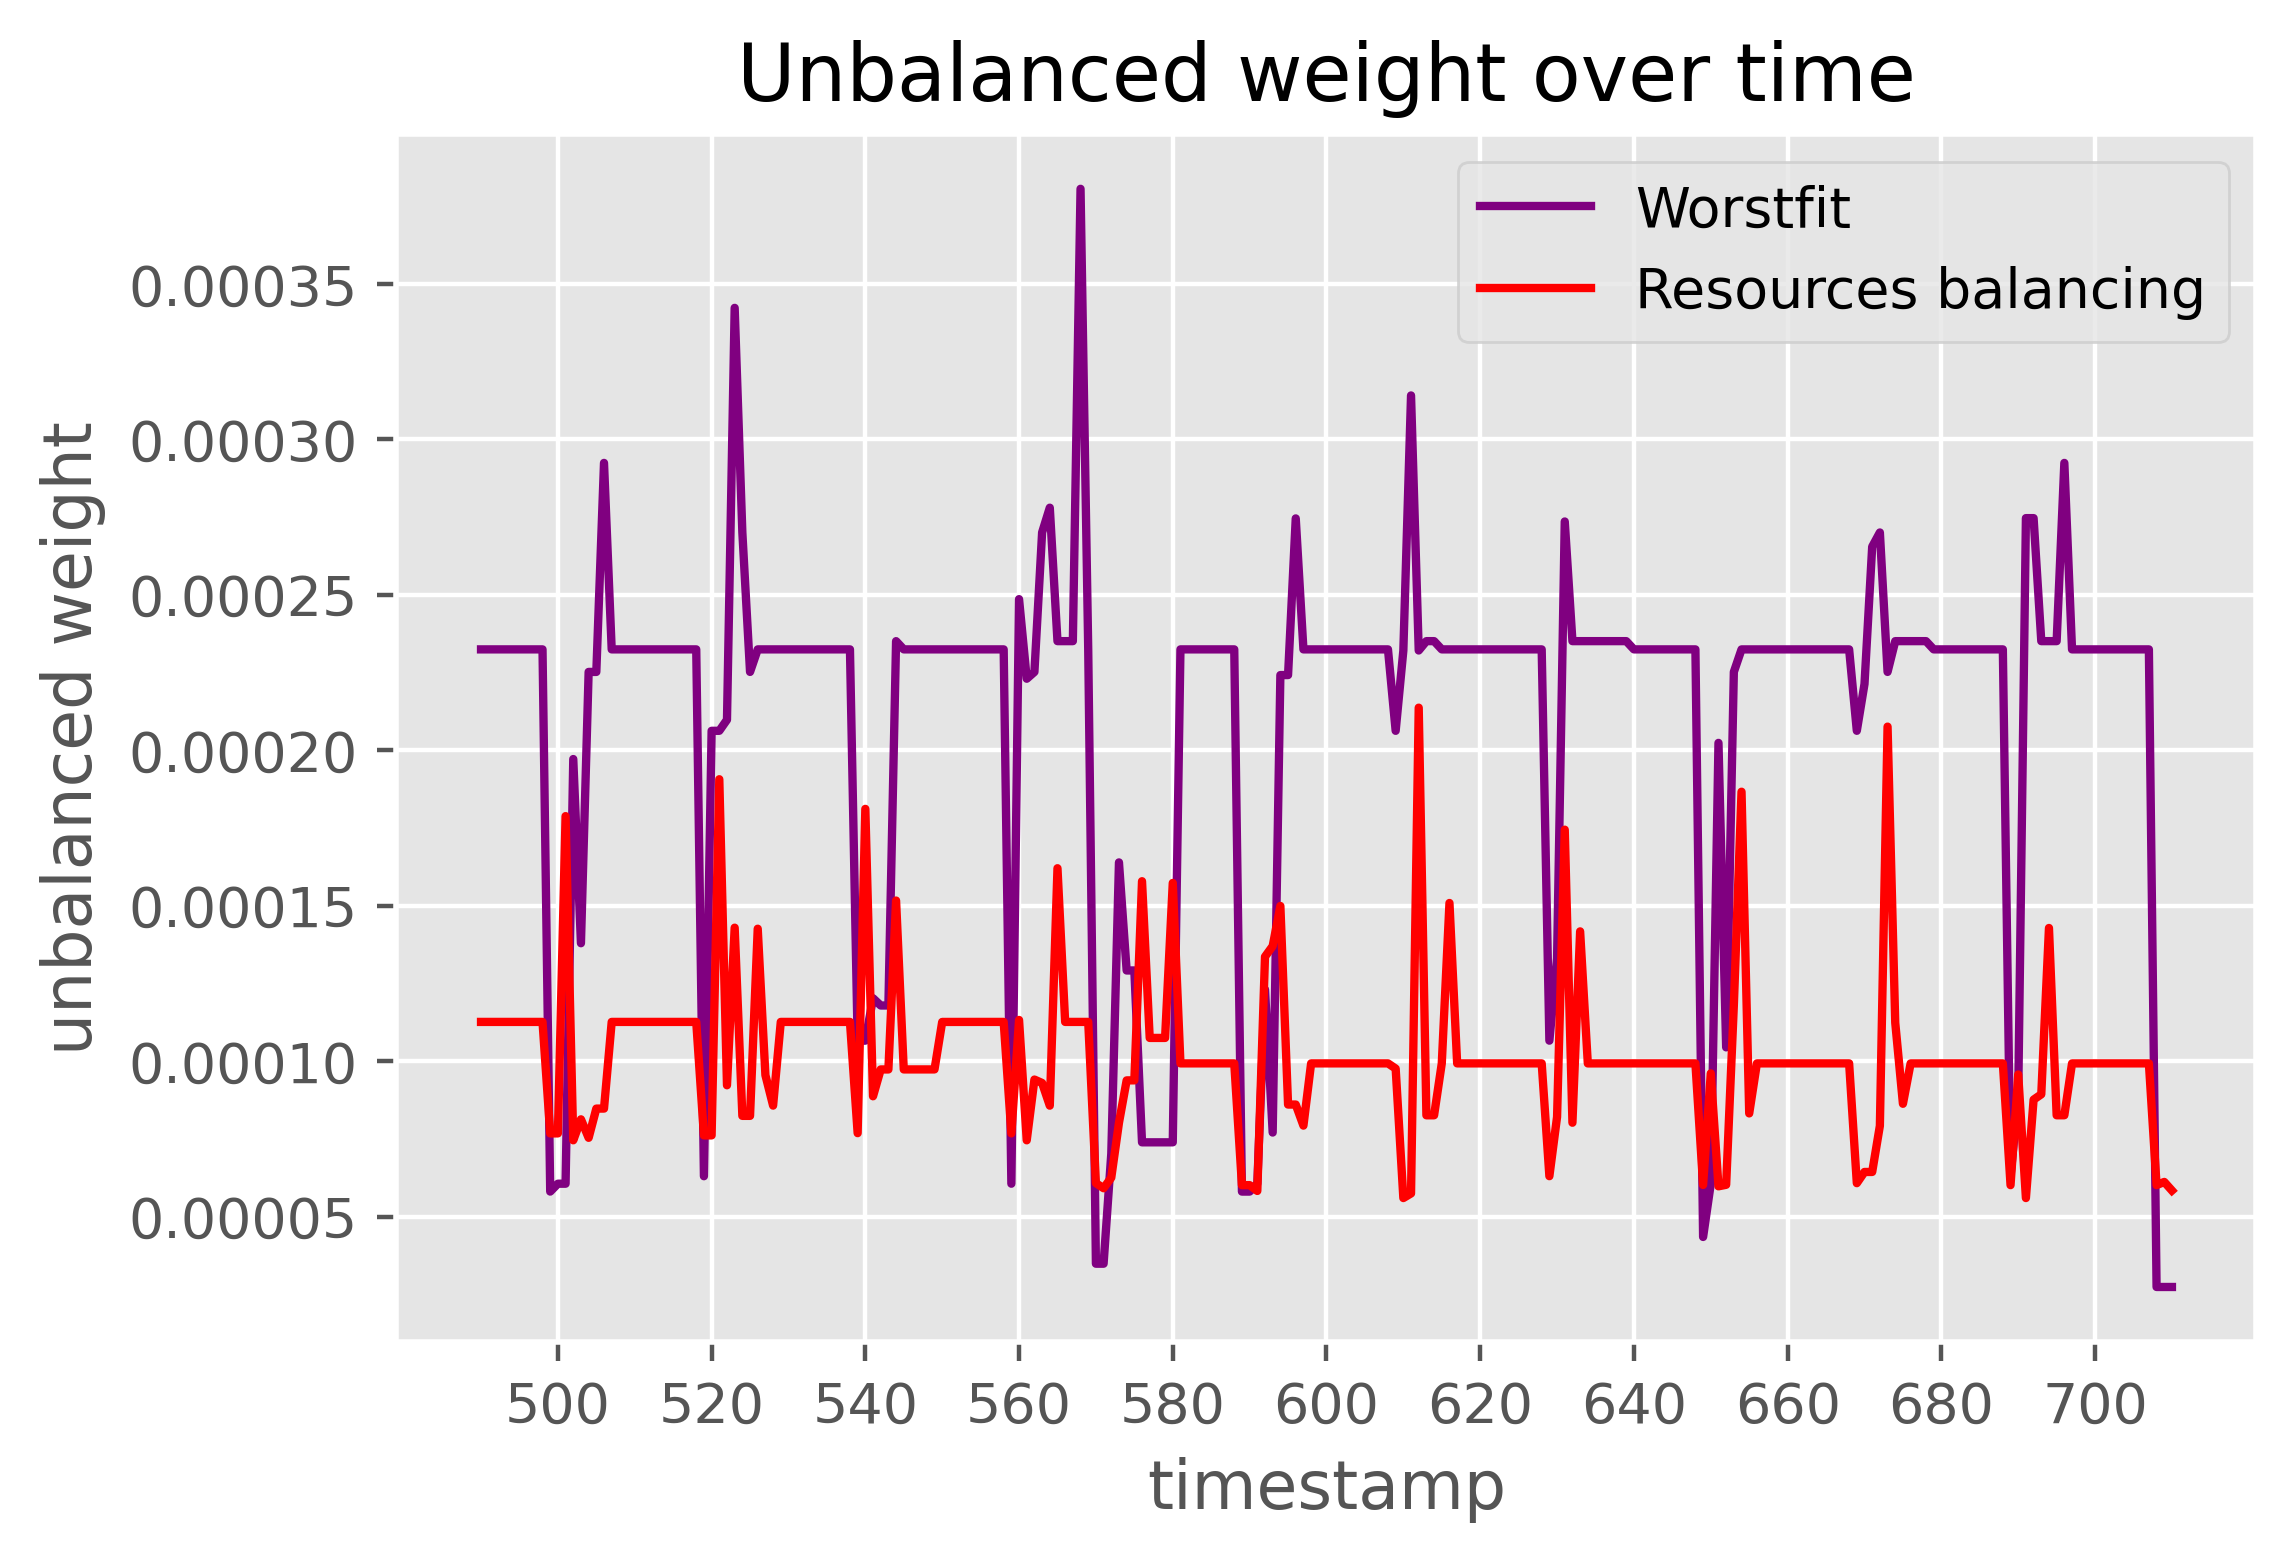
\includegraphics[scale=0.75]{images/unbalanced_weights.png}
	\caption{Mức độ mất cân bằng trong quá trình hoạt động}
	\label{fig:realtime_weights}
\end{figure}

\noindent
Như đã được đề cập ở~\ref{unload_balancing}, trạng thái các tasks thay đổi trong quá trình chạy là nguyên nhân dẫn đến sự mất cân bằng tài nguyên sử dụng giữa các máy.\\
Hình~\ref{fig:realtime_weights} thể hiện sự thay đổi trọng số mất cân bằng hệ thống (được tính toán trong thuật toán~\ref{alg:2} với tài nguyên CPU) theo thời gian của hai thuật toán Resources Balancing và Worstfit. Thuật toán Resources Balancing có sử dụng mạng Bayesian để ước lượng sự thay đổi của tài nguyên trong quá trình chạy để đưa ra quyết định lập lịch có thể thích ứng được với các sự thay đổi đó. Các tasks đến hệ thống và được đưa vào hàng đợi, cách 20 giây lập lịch một lần tại các thời điểm 500, 520, ... Tại các thời điểm lập lịch, ta thấy rằng chỉ số mất cân bằng của thuật toán Worstfit đôi khi tốt hơn so với thuật toán Resources Balancing, nhưng về tổng quan thì Resources Balancing tốt hơn. Bên cạnh đó, độ biến động của đường biểu thị cho Worstfit cũng cao hơn so với Resources Balancing. Điều này đúng với tính chất của thuật toán, do Worstfit chỉ tập trung tối ưu tại thời điểm lập lịch nên chỉ số tại thời điểm đó sẽ tốt hơn, nhưng trong quá trình chạy các tasks thay đổi trạng thái khiến cho sự cân bằng bị phá vỡ. Điều tương tự cũng xảy ra với Resources Balancing, nhưng hiệu quả của việc ước lượng tài nguyên với cân bằng giữa long-running tasks và batch-job tasks đã làm giảm độ biến động của chỉ số mất cân bằng, nên trong quá trình chạy trọng số của thuật toán này nhỏ hơn Worstfit. 

\newpage 
\chapter{Kết luận và định hướng nghiên cứu}
\label{Conclusion}
\section{Kết quả đạt được}
Dựa trên các phân tích thực nghiệm, đồ án này đạt được một số kết quả sau: 
\begin{itemize}
	\item Tăng số lượng tasks được hoàn thành trên đơn vị thời gian so với các thuật toán được sử dụng phổ biến ở các hệ thống máy chủ là Worstfit và FCFS.
	\item Giảm 50\% thời gian thực thi trung bình so với FCFS. 
	\item Cách dùng mạng Bayesian để cải thiện sai số do độ trễ trong quá trình lập lịch đưa ra thông số ước lượng sát với thực tế hơn so với việc dùng thông tin bị trễ. 
	\item Thuật toán đề xuất Resources Balancing giúp cân bằng tài nguyên sử dụng giữa các máy trong hệ thống cả trong quá trình chạy, vượt trội hơn so với việc chỉ cân bằng tại thời điểm lập lịch. 
\end{itemize}
Với kết quả như trên, đồ án đã hoàn thành 3 mục tiêu đặt ra: 
\begin{enumerate}
	\item Đưa ra các hạn chế của các thuật toán lập lịch như Worstfit trong môi trường Cloud 
	\item Nghiên cứu và đề xuất mô hình lập lịch cải tiến 
	\item Cài đặt, đánh giá, so sánh với các thuật toán khác 
\end{enumerate}
Việc sử dụng các mô hình ước lượng để tiếp cận các thành phần thay đổi liên tục trong hệ thống là một phương pháp khả thi, có thể mở rộng và cải tiến cho nhiều trường hợp phức tạp hơn. 
% 1-2 pages
\section{Định hướng nghiên cứu}
Với hiệu quả của phương pháp ước lượng các thành phần lập lịch, có ba hướng phát triển được đưa ra như sau: 
\begin{enumerate}
	\item Trong thực tế, các tasks có thể có quan hệ cha con. Các quan hệ này được biểu diễn dưới dạng cây, kèm theo các rằng buộc giữa chúng. Ta có thể xây dựng đồ thị Bayesian dạng cây tương tự để có thể ước lượng chính xác hơn. 
	\item Trong thời gian hoạt động, các tasks được gửi đến hệ thống theo dạng streaming. Để thích ứng với sự thay đổi của dữ liệu, mô hình Bayesian cần được học liên tục theo luồng dữ liệu chạy trong hệ thống. Việc cân bằng giữa tri thức học được từ quá khứ với tri thức học được hiện tại sẽ giúp mô hình đưa ra dự đoán chính xác hơn.
	\item Ngoài việc tối ưu về thời gian và độ cân bằng sử dụng tài nguyên giữa các máy ảo, ta còn có thể tối ưu năng lượng sử dụng, đưa thêm các ràng buộc về máy ảo, các máy ảo có thể chuyển trạng thái từ bật sang tắt để mở rộng hoặc thu hẹp hệ thống. Trong trường hợp này, nếu có thể ước lượng được tài nguyên cần thiết thì có thể đưa ra số lượng máy tính cần hoạt động nhỏ nhất để tối ưu năng lượng tiêu thụ. 
\end{enumerate}

\newpage
\medskip
\printbibliography[title={Tài liệu tham khảo}]

\newpage 

\end{document}
